\documentclass[svgnames,dvipsnames,a4paper,10pt,french]{report}
\usepackage{centrale}

\DeclareGraphicsRule{.ai}{pdf}{.ai}{} % pour insérer des documents .ai
\graphicspath{ {./images/} {./eps/}} % pour ne pas avoir à ajouter eps/ton-image.jpg

\usepackage[toc,page]{appendix}
\renewcommand\appendixtocname{Annexes}

\renewcommand\appendixname{Annexes}
\renewcommand\appendixpagename{Annexes}


\usepackage[normalem]{ulem}
\useunder{\uline}{\ul}{}

\graphicspath{ {images/} }
\usepackage{enumitem}
\usepackage{float}
\usepackage{wrapfig}
\setlength{\parskip}{.5em}

\usepackage{epigraph}
\usepackage{spverbatim}
\usepackage{xurl}
\usepackage{amsmath}%
\usepackage{subfig}
\usepackage{dsfont} % pour le \mathds{I}
\usepackage{stmaryrd} % pour llbracket et rrbracket
\usepackage{mathrsfs}  
\usepackage[autostyle=false, style=french]{csquotes}
% \usepackage{unicode-math} % pour julia latex
\usepackage{bm}
\usepackage{amsbsy}
\usepackage{booktabs}
%\setmonofont{DejaVu Sans Mono}[Scale=MatchLowercase]
\usepackage{minted}
\usepackage{fontspec}
% \usepackage{kbordermatrix} % https://tex.stackexchange.com/questions/59517/label-rows-of-a-matrix-by-characters pour faire des légendes sur les matrices
\usepackage{kbordermatrix,blkarray}

\renewcommand{\kbldelim}{(}
\renewcommand{\kbrdelim}{)}


\usepackage{nicematrix}
\NiceMatrixOptions{
code-for-first-row = \color{blue} ,
code-for-last-row = \color{blue} ,
code-for-first-col = \color{blue} ,
code-for-last-col = \color{blue}
}


% \usepackage{newunicodechar}





\usepackage{algorithmicx}
\usepackage{algorithm}
\usepackage{algpseudocode}
\newenvironment{breakablealgorithm} % https://tex.stackexchange.com/questions/33866/algorithm-tag-and-page-break
  {% \begin{breakablealgorithm}
   \begin{center}
     \refstepcounter{algorithm}% New algorithm
     \hrule height.8pt depth0pt \kern2pt% \@fs@pre for \@fs@ruled
     \renewcommand{\caption}[2][\relax]{% Make a new \caption
       {\raggedright\textbf{\fname@algorithm~\thealgorithm} ##2\par}%
       \ifx\relax##1\relax % #1 is \relax
         \addcontentsline{loa}{algorithm}{\protect\numberline{\thealgorithm}##2}%
       \else % #1 is not \relax
         \addcontentsline{loa}{algorithm}{\protect\numberline{\thealgorithm}##1}%
       \fi
       \kern2pt\hrule\kern2pt
     }
  }{% \end{breakablealgorithm}
     \kern2pt\hrule\relax% \@fs@post for \@fs@ruled
   \end{center}
  }
\makeatother

 % https://tex.stackexchange.com/questions/569777/why-do-i-get-require-and-ensure-instead-of-input-and-output-phrases-in-m
\algrenewcommand\algorithmicrequire{\textbf{Input:}}
\algrenewcommand\algorithmicensure{\textbf{Output:}}
%\usepackage[linesnumbered,ruled,vlined]{algorithm2e}


\usepackage{tikz}
\newcommand*\circled[1]{\tikz[baseline=(char.base)]{\node[shape=circle,draw,inner sep=2pt] (char) {#1};}}

\newcommand*{\TakeFourierOrnament}[1]{{%
\fontencoding{U}\fontfamily{futs}\selectfont\char#1}}
\newcommand*{\danger}{\TakeFourierOrnament{66}}

\newenvironment{codejulia}[1]
{
  \VerbatimEnvironment
  \begin{listing}[H]
  \begin{minted}[%
      label = #1,%  Might want to change or remove this label
      linenos,
      breaklines,
      style = paraiso,
      fontsize=\small,
      frame = single,
      escapeinside=||,
      mathescape=true,
      baselinestretch=.7,
      framesep=2mm,
      ]{julia}
}
{
  \end{minted}%
  \end{listing}%
}



\usepackage{amsthm} % pour les théorèmes, preuves, etc
%\usepackage{ntheorem} % pour revenir à la ligne avec la commande suivante (mais attention ne contient pas proof)

%\theoremstyle{break}

\renewcommand\qedsymbol{$\blacksquare$} % pour changer le symbole en fin de preuve



\newcommand\myeq{\stackrel{\mathclap{\normalfont\tiny\mbox{def}}}{=}}

\newtheorem{theorem}{Théorème}[section]
\newtheorem{corollary}{Corollaire}[theorem]
\newtheorem{lemma}[theorem]{Lemme}
\newtheorem{acknowledgement}[theorem]{Acknowledgement}
% \newtheorem{algorithm}[theorem]{Algorithme}
\newtheorem{axiom}[theorem]{Axiome}
\newtheorem{case}[theorem]{Cas}
\newtheorem{claim}[theorem]{Assertion}
\newtheorem{conclusion}[theorem]{Conclusion}
\newtheorem{condition}[theorem]{Condition}
\newtheorem{conjecture}[theorem]{Conjecture}
\newtheorem{criterion}[theorem]{Critère}
\newtheorem{definition}[theorem]{Définition}
\newtheorem{example}[theorem]{Exemple}
\newtheorem{exercise}[theorem]{Exercice}
\newtheorem{notation}[theorem]{Notation}
\newtheorem{propriety}[theorem]{Propriété}
\newtheorem{problem}[theorem]{Problème}
\newtheorem{proposition}[theorem]{Proposition}
\newtheorem{remark}[theorem]{Remarque}
\newtheorem{solution}[theorem]{Solution}
\newtheorem{summary}[theorem]{Résumé}




\hypersetup{
    colorlinks=true,
    %linkbordercolor=red,
    linkcolor=red,
    urlcolor=cyan,
    citecolor=blue,
    pdftoolbar=false,        % show Acrobat’s toolbar?
    pdfmenubar=true,        % show Acrobat’s menu?
    pdffitwindow=false,     % window fit to page when opened
    pdfstartview={FitH},    % fits the width of the page to the window
    pdfnewwindow=true,      % links in new PDF window
    pdfcreator={Paquet LaTeX Centrale Lyon (B. Laville) - 2019}
}





\usepackage[fixlanguage]{babelbib}


\begin{document}
\NewDocumentCommand{\codeword}{v}{\texttt{#1}}


\newcommand{\codewordred}[1]{\texttt{\textcolor{DarkRed}{#1}}}
\newcommand{\codewordblue}[1]{\texttt{\textcolor{blue}{#1}}}
\newcommand{\codewordgreen}[1]{\texttt{\textcolor{ForestGreen}{#1}}}
\newcommand*{\I}{\mathrm{i}}
\newcommand{\vect}[1]{\mathbf{#1}}
% \newcommand{\ref}[1]{\textbf{\textcolor{CentraleRed}{\textsc{\ref{#1}}}}}  % Pour réaliser des citations potables

% \newcommand{\eqdef}{\stackrel{\mathrm{def}}{=}}
\newcommand{\argmax}{\operatornamewithlimits{argmax}}
\newcommand{\argmin}{\operatornamewithlimits{argmin}}
\begin{titlepage}
\begin{center}

\includegraphics[width=1\textwidth]{logo_ECL_rectangle_quadri_vectoriel.ai}\\[1cm]

{\Large UE PRO tc2 2021-2022 -- Stage Application}\\[0.5cm]



% Title
\rule{\linewidth}{0.5mm} \\[0.4cm]
{\huge  Simulation numérique d'équations de \textsc{Schrödinger}}\\[0.4cm]
\rule{\linewidth}{0.5mm} \\[1.5cm]

{\large Stage effectué du 19 avril 2022 au 12 août 2022 au Centre d’Enseignement et de Recherche en MathématIques et Calcul Scientifique (CERMICS) à l'École des Ponts et Chaussées ParisTech}\\[0.5cm]


\includegraphics[scale=.35]{5-ecole_ponts20_rvb72petit.jpg}\\[1cm]


% Author and supervisor
\noindent
\begin{minipage}{0.4\textwidth}
  \begin{flushleft} \large
    \emph{Auteur :}\\
    \vspace{.3cm}
    Matthias \textsc{Personnaz} (ECL20)
  \end{flushleft}
\end{minipage}%
\begin{minipage}{0.6\textwidth}
  \begin{flushright} \large
    \emph{Encadrants :} \\
    \vspace{.3cm}
    Éric    \textsc{Cances} (référent scientifique, ENPC) \\
    Giacomo \textsc{Casadei} (référent pédagogique, ECL)
  \end{flushright}
\end{minipage}



\vfill
\selectlanguage{french} 
% Bottom of the page
{\large Version compilée le\\ \today}

\end{center}
\end{titlepage}
\thispagestyle{empty}

\renewcommand*\contentsname{Sommaire}
\renewcommand{\listalgorithmname}{Liste des algorithmes}


\selectlanguage{french} 
\begin{abstract}
    Ce document est un rapport de stage application effectué dans le cadre du cursus \og Ingénieur Généraliste \fg{} de l'École Centrale de Lyon. Il décrit la structure d'accueil, le travail effectué, ainsi que les perspectives en regard du processus de construction du projet professionnel. Le travail de ce stage, proposé par le tuteur scientifique, consiste à tester numériquement dans un cadre simplifié les limites de l’approximation de Born-Oppenheimer utilisée en simulation moléculaire pour découpler la dynamique des électrons de celle des noyaux atomiques, sans avoir à résoudre un problème bidimensionnel trop coûteux numériquement. 
    Pour y parvenir, mis en \oe{}uvre la théorie des perturbations en Julia, en justifiant chaque fois le mieux possible les hypothèses mathématiques utilisées, leur cadre de validité, ainsi que les choix de conception. Avec la méthode employée, je montre que la complexité asymptotique des perturbations sous certaines hypothèses est $\mathcal{O}\left(N \sqrt{E_\text{max}(N)} \ln(E_\text{max}(N)) \right)$ avec $N$ la dimension de l'espace de \textsc{Hilbert} discret approchant le problème (taille de la grille) et $E_\text{max}$ l'énergie maximale approchée sur cet espace. Les résultats numériques montrent que l'inégalité de \textsc{Kato-Temple} ne donne pas d'information utile. Enfin, en parallèle, en utilisant les bibliothèques de Julia, j'ai mis au point une heuristique en programmation dynamique généralisable à tout algorithme calculatoire pour alterner de manière optimale entre CPU et GPU. Ce travail de conception et de programmation pourra servir de base pour de futurs codes servant à évaluer de manière plus poussée les états propres de systèmes moléculaires complexes.
    
\end{abstract}
\selectlanguage{english}
\begin{abstract}
  This document is a report on an internship carried out as part of the  Engineering program at the École Centrale de Lyon. It describes the host structure, the work carried out, as well as the perspectives with regard to the process of building a professional project. The work of this internship, proposed by the scientific tutor, consists in numerically testing in a simplified framework the limits of the Born-Oppenheimer approximation used in molecular simulation to decouple the dynamics of electrons from those of atomic nuclei, without having to solve a two-dimensional problem that is too costly numerically. 
  In order to achieve this, I implement the theory of perturbations in Julia, and justified the mathematical assumptions used as well as possible, along with their framework of validity and the design choices. With the chosen method, I show that the asymptotic complexity of the perturbations under certain assumptions is $\mathcal{O}\left(N \sqrt{E_\text{max}(N)} \ln(E_\text{max}(N)) \right)$ with $N$ being the dimension of the discrete \textsc{Hilbert} space approximating the problem (grid size) and $E_\text{max}$ the maximum energy approximated on this space. Numerical results show that the \textsc{Kato-Temple} inequality does not give useful information. Finally, in parallel, using Julia's libraries, I have developed a dynamic programming heuristic that can be generalized to any computational algorithm to optimally alternate between CPU and GPU uses. This design and programming work can serve as a basis for future codes to further evaluate the eigenstates of complex molecular systems.



\end{abstract}
\selectlanguage{french}

\section*{Remerciements}
Je remercie
\begin{itemize}
    \item Éric Cances (professeurs à l'ENPC, chercheur au CERMICS, tuteur scientifique) pour m'avoir accordé sa confiance en me sélectionnant pour ce stage, et expliqué ses aspects physiques et mathématiques, ainsi que pour ses indications à propos des méthodes préférentielles de l'état de l'art;
    \item Paul Cazeaux (professeur et chercheur à l'université du Kansas) pour ses conseils pertinents permettant d'améliorer la complexité des algorithmes lors de notre rencontre à Roscoff;
    \item Laurent Vidal (doctorant au CERMICS) pour ses conseils pratiques sur la programmation en Julia qui m'ont permis de gagner du temps au débuggage.
\end{itemize}



\vspace{6cm}
Dans ce document, les bibliothèques sont notées en rouge (comme \codewordred{KrylovKit}), les classes en bleu (comme \codewordblue{CUDA.CUSPARSE}), et les fonctions en vert (par exemple, \codewordgreen{eigvecs} ou \codewordgreen{eigvals}).


Les codes qui ont servi à la génération des figures de ce rapport, ainsi que résoudre le problème posé en général, sont disponibles à l'adresse  \url{https://github.com/MatthiasPersonnaz/stage_CERMICS_BO}.



{
  \hypersetup{linkcolor=black}
  \tableofcontents
  \listoffigures
  \listoftables
  \listofalgorithms
}






\newpage


\chapter{Présentation du cadre du stage, de l'école des Ponts ParisTech et du CERMICS}

\section{Contexte du stage}
L'École des Ponts ParisTech est une grande école d'ingénieurs française, accréditée par la Comission des Titres d'Ingénieurs (CTI), fondée en 1747. Elle est ainsi l'une des plus anciennes écoles d'ingénieurs françaises. Elle se situe géographiquement à Champ-Sur-Marne en Seine-et-Marne (région Île-de-France), attenante à l'université \textsc{Gustave Eiffel} et à l'école nationale supérieure de géomatique (ENSG). Historiquement, ses domaines d'expertise étaient le génie civil et de l'aménagement du territoire, mais elle en a développé au cours des années de nombreux autres. En particulier, son activité comporte une forte composante de recherche avec 12 laboratoires de recherche sur les domaines des sciences de l'environnement, de l'économie, des mathématiques et informatique et de la dynamique des fluides principalement.

Mon stage se déroulait au laboratoire CERMICS (Centre d’Enseignement et de Recherche en Mathématiques et Calcul Scientifique) dirigé par Tony \textsc{Lelièvre} à l'heure de rédaction de ce rapport, physiquement lui-même situé sur le site de l'ENPC, qui organise ses recherche autour des thématiques  de modélisation en probabilités, de l'optimisation, de la recherche opérationnelle et de simulation numérique. 

Plus particulièrement, je me trouvais dans l'équipe de simulation, composée de 11 chercheurs permanents en septembre 2022, dont mon tuteur scientifique, \textsc{Éric Cances}. Le stage s’inscrivait dans le cadre du projet ERC Synergy EMC2 (\url{https://erc-emc2.eu}) qui vise à surmonter certaines des limites actuelles dans le domaine de la simulation moléculaire et à développer pour la communauté universitaire des logiciels de simulation moléculaire de plus efficaces et plus fiables. Parmi les activités de recherche les plus présentes, on peut citer le travail effectué par l'équipe de recherche MATHERIALS, constituée de chercheurs au CERMICS et à l'INRIA Paris, qui est impliquée dans les calculs de structure électronique dans de nombreux problèmes de  chimie quantique et de dynamique moléculaire.

Mon travail s'inscrivait ainsi dans la lignée parfaite des activités de recherche menées au laboratoire avec toutefois un sujet bien plus simpliste.

Parmi les permanents du laboratoire, on peut dénombrer de nombreux ingénieurs de formation en proportion des chercheurs, la plupart d'entre eux étant polytechniciens et/ou ingénieurs de l'École des Ponts. Je n'ai pas pu en revanche côtoyer beaucoup les chercheurs (hormis mon propre tuteur), car une partie travaille aussi dans plusieurs laboratoires gravitant autour de Paris (avec des équipes notamment dans les universités de Paris comme la Sorbonne ou Jussieu), voire en séminaires et en collaboration à l'étranger, et sont occupés à leur recherche conjointement avec leurs étudiants en thèse ou propres stagiaires sous leur direction. D'une manière générale la recherche, et particulièrement la recherche en mathématique, est un domaine très mondialisé avec une forte composante de collaboration internationale.

Il faut aussi compter que mon stage ayant été planifié d'avril à août, dès le début de la période estivale, l'activité est mécaniquement réduite par rapport aux temps forts qui interviennent à chaque rentrée universitaire sur le campus des Ponts, avec au programme de nombreux colloques, séminaires internes et activités de collaboration. De plus, les réminiscences du Covid-19 ont aisément ancré une habitude de télétravail probablement plus importante que quelques années auparavant, puisque l'activité de recherche en mathématiques appliquées et simulation s'y prête bien.

Pendant le stage, j'ai été invité à participer à une rencontre scientifique du 17 au 22 juillet 2022 à Roscoff, pendant laquelle des chercheurs du CERMICS, du LCT (Laboratoire de Chimie Théorique, à la Sorbonne) et de l'INRIA discutent ensemble de directions communes de recherches, travaillent sur leurs modèles, etc.  Cette occasion m'a permis de comprendre mieux comment s'articule la recherche autour de plusieurs acteurs et plusieurs laboratoires, et de côtoyer des personnes issues de formations assez différentes de celles que j'avais pu majoritairement voir jusqu'alors, principalement universitaires. J'ai rencontré plusieurs jeunes chercheurs en thèse de master, en doctorat ou fraîchement maîtres de conférence. J'ai pu notamment les questionner sur certaines techniques utilisant du Machine Learning pour résoudre des problèmes de chimie quantique, ce qui a résonné avec mon PAr effectué à l'ECL quelques mois auparavant. 

\section{Organisation du travail}

Comme déjà évoqué, la recherche, au moins au sein des équipes, est hautement collaborative. Les chercheurs se partagent les tâches, partagent leur expériences et leurs expertises. En témoignent les nombreux articles publiés ou en pré-publication co-signés par souvent au moins deux permanents du laboratoire, voire avec des chercheurs d'autres laboratoires extérieurs. C'est également, je crois, un domaine où la liberté et la flexibilité dans l'organisation et la direction choisie du travail est plus élevée en moyenne que dans les entreprises. Généralement, la recherche part de résultats antérieurs que l'on essaie d'améliorer, ou au contraire d'absence de résultats, auquel cas on essaie de créer un modèle, de l'expliquer, de l'améliorer, etc. Ce que je décris là est néanmoins tout-à-fait classique et c'est le mécanisme qui se joue dans la recherche en sciences depuis des siècles.

\subsection{Polarisation de la recherche par domaines}
Le CERMICS et les laboratoires associés est le lieu de France par l'équipe MATHERIALS, a pu développer au fil des années une expertise solide \og de niche \fg{} traditionnellement assez peu explorée ou connue par le reste de la communauté internationale.\footnote{Source: rapport d'activité de MATHERIALS \url{https://raweb.inria.fr/rapportsactivite/RA2019/matherials/matherials.pdf}}

À Roscoff, une différence qui m'a alors positivement frappé était combien les étudiants en masters orientés en mathématiques-informatique disposent d'une expertise sur certains domaines très pointus et précis qui sont structurellement absents de la formation d'ingénieur que j'ai reçue à l'ECL à niveau de formation égal. Ces masters proposent une offre de cours sur des sujets pointus qui n'existent simplement pas ou peu ailleurs (ce que m'ont informellement confirmé  des étudiants en thèse). Un exemple éloquent: certains cours de calcul haute performance à très bas niveau (très proche de la machine) ne sont susceptibles d'être enseignés dans peu d'écoles d'ingénieurs françaises à niveau d'études équivalent), et majoritairement absent voire totalement inexistant des options informatique de certaines écoles du GEC\footnote{Groupe des Écoles Centrale} au même niveau d'études (M1). Ce simple détail montre bien à quel point l'activité de recherche est très polarisée par domaine et avec elle, la formation usuelle préalable, vis-à-vis de la géographie en France (et dans le monde également). Ce constat fait écho à un intérêt que j'ai pour l'organisation de l'enseignement supérieur et de la recherche dans le monde. Pour étayer ces propos qui ne sont qu'au stade de l'intuition, il faudrait cependant mener une étude plus aboutie en sociologie de la recherche et peut-être en épistémologie mais ne s'agissant pas du propos principal, j'élude ici le sujet.




\begin{figure}
    \centering
    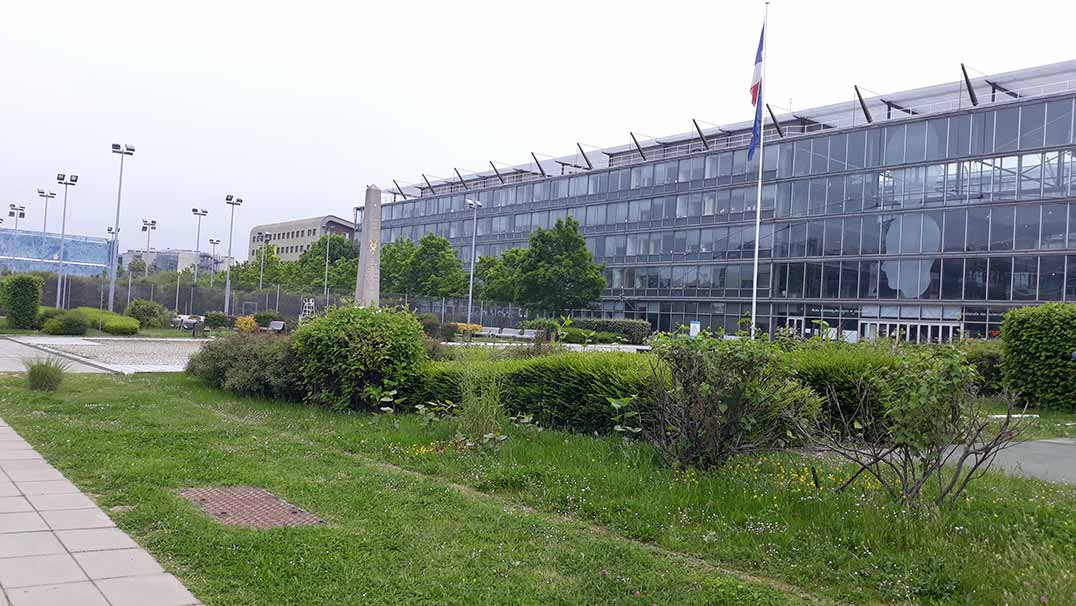
\includegraphics[width=.7\textwidth]{images/esplanade.jpg}
    \caption{Esplanade devant l'école des Ponts et l'école nationale supérieure de géomatique, dont les bâtiments partagés sont visibles à l'arrière-plan.}
    \label{fig:explanade}
\end{figure}

\begin{figure}
    \centering
    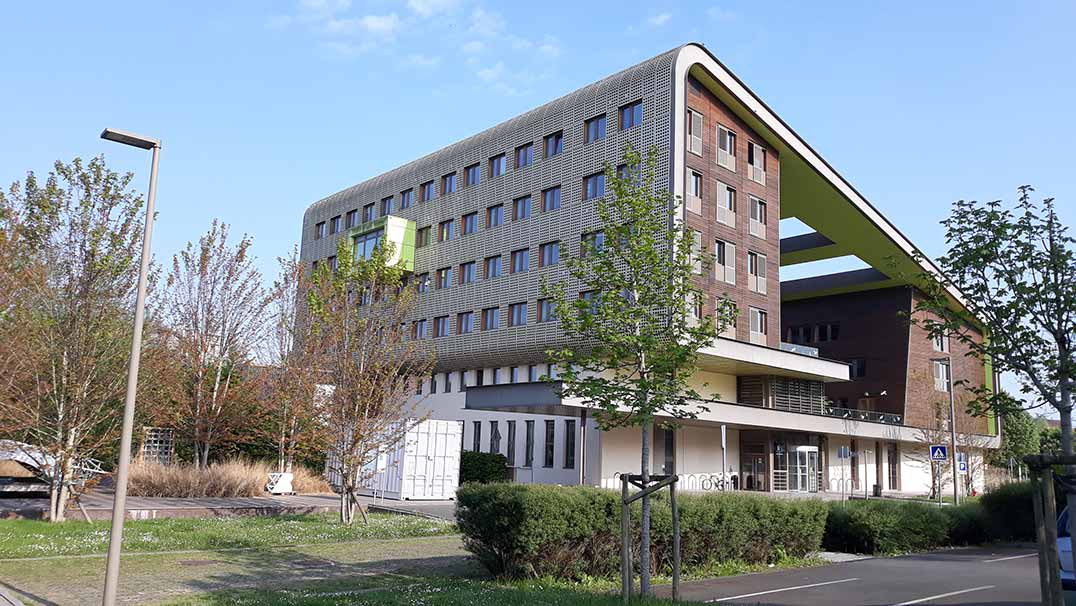
\includegraphics[width=.7\textwidth]{images/coriolis.jpg}
    \caption{Bâtiment Coriolis, abritant le CERMICS.}
    \label{fig:explanade}
\end{figure}


\chapter{Généralités en physique quantique, sous-jacents en simulation numérique et introduction du problème}


\section{Position du problème}
Rappelons très succintement quelques éléments qui mettent en contexte le travail effectué lors de ce stage. La plupart de ce chapitre est fortement inspiré de, et résume certains des points importants de, \cite{cohen-tannoudji_mecanique_2021} et \cite{cances_introduction_2021} et constitue un résumé de généralités en quantique\footnote{Qui prolonge en particulier les notions effleurées dans les  UEs PCM, GM et IDM du programme de l'ECL.} et sert à poser un cadre clair. Une partie importante du travail de ce stage a consisté à se familiariser avec, et étudier les fondements de la physique quantique au travers d'ouvrages de référence et d'articles jusqu'au niveau L3 environ, mais évidemment le but n'est pas ici de recopier ces cours et la littérature en entier, seulement d'en exposer les éléments les plus importants que j'ai dû m'approprier.


\subsection{Fondamentaux succints sur le formalisme utilisé et le sens physique des simulations}


\subsubsection{Mécanique classique}
En mécanique classique, le mouvement d'un système matériel quelconque peut se décrire notamment à l'aide du formalisme lagrangien qui met en jeu des coordonnées généralisées appelées \emph{variables dynamiques fondamentales}, notées traditionnellement $q_i$. Le \textbf{lagrangien} $\mathcal{L}(q_i,\dot{q_i},t)$ est une grandeur associée au système qui est la différence $E_c-E_p$. À ces coordonnées on associe également les \emph{moments conjugués} $p_i = \frac{\partial \mathcal{L}}{\partial \dot{q_i}}$. Le \textbf{hamiltonien} donne l'énergie totale du système de points matériels $\mathcal{H}(p_i,q_i,t)$ et son évolution est dicté par les équations de \textsc{Hamilton-Jacobi}:

\begin{equation}
    \begin{array}{ll}
        \frac{\mathrm{d}q_i}{\mathrm{d}t} &= +\frac{\mathrm{d}\mathcal{H}}{\mathrm{d}p_i} \\
        \frac{\mathrm{d}q_i}{\mathrm{d}t} &= -\frac{\mathrm{d}\mathcal{H}}{\mathrm{d}q_i}
    \end{array}
\end{equation}

Pour un point matériel seul, les trois variables dynamiques sont les trois coordonnées de l'espace constituant le vecteur $\vect{r}$, et l'énergie totale du système s'écrit 
\begin{equation}
    \mathcal{H} = \frac{\vect{p}^2}{2m} + V(\vect{r} ,t)
\end{equation}
et les équations de \textsc{Hamilton-Jacobi} prennent la forme connue

\begin{equation}
    \begin{array}{ll}
        \frac{\mathrm{d}\vect{r}}{\mathrm{d}t} &= \frac{\vect{p}}{m} \\
        \frac{\mathrm{d}\vect{p}}{\mathrm{d}t} &= -\nabla(V)
    \end{array}
\end{equation}



\subsubsection{Mécanique quantique}
La meilleure théorie dont nous disposons qui puisse décrire le comportement fondamental de particules à des échelles très réduites est la physique quantique. À ces échelles, la mécanique classique ne fonctionne pas, mais certaines lois peuvent se vérifier en moyenne avec l'espérance de certains opérateurs. Avec les relations de \textsc{De Broglie} on associe à un corpuscule matériel d’énergie $P$ et d’impulsion $\vect{p}$, une onde dont la pulsation $\omega = 2 \pi\nu$ et le vecteur d’onde $\vect{k}$ sont donnés par les mêmes relations que pour les photons:
\begin{equation}
        \left\{\begin{array}{rcl}
        E &= h \nu &= \hbar \omega \\
        \vect{p} &= \hbar \vect{k} &
    \end{array}\right.
\end{equation}
Elle repose sur un formalisme et des postulats particuliers. Les postulats de la mécanique quantique stipulent notamment que :
\begin{itemize}
    \item Un état quantique d'une particule à un instant donné est caractérisé par une fonction d'onde $|\psi(t) \rangle$ (un \emph{ket} pour reprendre la notation de \textsc{Dirac}) qui appartient à un espace de \textsc{Hilbert} \mathscr{H} (c'est-à-dire un espace préhilbertien complexe, muni d'un produit scalaire hermitien et de la norme associée), dont une facteur de phrase $e^{i\theta}$ n'affecte pas le sens physique. Cette fonction peut varier dans l'espace et le temps, on la note aussi $\psi(\vect{},t)$. En chaque endroit de l'espace accessible à la particule, $|\psi(\vect{x},t)|^2$ est la densité de probabilité de présence de la particule.
    \item Toute grandeur physique d'intérêt, mesurable, est décrite par un opérateur $\mathcal{A}$ agissant dans l'espace des états: cet opérateur est appelé \textbf{observable}.
    \item Les valeurs permises pour cette grandeur physique sont les valeurs propres de l'opérateur $\mathcal{A}$, i.e. les nombres $A$ tels que $\mathcal{A}|\psi \rangle = A |\psi\rangle$. Le spectre d'un observable peut également être continu ou discret. En outre la probabilité d'observation de chaque valeur n'est pas nécessairement également distribuée parmi toutes les valeurs permises.
    \item L'évolution de la fonction d'onde dans le temps est régie par l'équation de \textsc{Schrödinger}
    \begin{equation}
    \label{schrodinger}
        \I\hbar \frac{\partial}{\partial t} |\psi(t) \rangle = \hat{H}(t) |\psi(t) \rangle
    \end{equation} où $\hat{\mathcal{H}}$ est l'\textbf{opérateur hamiltonien}, associé à l'observable énergie totale du système et s'écrit
    \begin{equation}
    \label{energie_totale_hamiltonien}
        \hat{\mathcal{H}} = -\frac{\hbar^2}{2m} \Delta + \hat{V}(\vect{r}) = \frac{\vect{p}^2}{2m} \Delta + \hat{V}(\vect{r})
    \end{equation} où $\vect{p} = -\I\hbar \vect{\nabla}$ est l'opérateur \textbf{impulsion}.
\end{itemize}  

\paragraph{États stationnaire}
Lorsque le hamiltonien du système ne dépend pas du temps, une fonction d'onde de la forme
\begin{equation}
\label{solution_separable}
    |\psi(\vect{r},t)\rangle = |\phi(\vect{r}) \rangle \chi (t) 
\end{equation}
correspond à un état \textbf{stationnaire} de la fonction d'onde, de densité de probabilité indépendante du temps. Un tel état est d'énergie bien définie. La résolution, très courante, consiste à réinjecter \ref{solution_separable} dans \ref{schrodinger} et séparer les variables:
 
 \begin{equation}
    \I \hbar |\phi(\vect{r})\rangle \frac{\mathrm{d}\chi}{\mathrm{d}t}(t) = \chi(t)\hat{H} |\phi(\vect{r})\rangle
 \end{equation}
 et séparer les variables des fonctions correspondantes aux états:
 \begin{equation}
     \I \hbar \frac{1}{\chi(t)} \frac{\mathrm{d}\chi}{\mathrm{d}t}(t) = \frac{1}{\phi(\vect{r})}\hat{H} \phi(\vect{r})
 \end{equation}
 comme chacun des deux membres ne dépend pas des variables présentes dans l'autre, l'équation est égale à une constante homogène à une énergie, que l'on désigne par $E$. L'équation différentielle qui s'en suit pour $\chi$ conduit à 
 
 \begin{equation}
     \psi(\vect{r},t) = \exp \left( -\I\frac{E}{\hbar} t \right) \phi(\vect{r})
 \end{equation}

 où $\phi$ est normée dans vérifie 
\begin{equation}
\label{eq:schrodinger_stationnaire}
    \hat{\mathcal{H}} \phi = E \phi
\end{equation}

$\hat{H}$ étant un opérateur linéaire, si l'on peut en particulier trouver un base orthonormale dénombrable pour le produit scalaire hermitien, de l'ensemble des solutions au problème \ref{eq:schrodinger_stationnaire}, de valeurs propres $E_n$ et de vecteurs $\phi_n$ associés, alors toute solution peut se décomposer de manière unique sous la forme
\begin{equation}
    \psi (\vect{r},t) = \sum_n c_n \phi_n(\vect{r}) e^{-iE_n t/\hbar} \text{ avec } \sum_n |c_n|^2 = 1
\end{equation}
où les $c_n$ sont des constantes complexes quelconques. C'est le cas par exemple pour l'oscillateur harmonique 1D dont on connait, grâce aux polynômes de \textsc{Hermite} et une démonstration dûe à \textsc{Dirac}. 


\paragraph{États liés et états de diffusion}
On appelle un état lié un état $|\psi \rangle$ tel que 
\begin{equation}
    \int_{\mathbb{R}^d} |\psi|^2(\vect{x}) \mathrm{d} \vect{x} = 1
\end{equation}
tandis qu'un état de diffusion est un vecteur propre tel que
\begin{equation}
    \int_{\mathbb{R}^d} |\psi|^2(\vect{x}) \mathrm{d} \vect{x} = +\infty
\end{equation}



Ce stage fait beaucoup usage du résultat suivant:

\begin{theorem}
\label{bo_osc_harm}
Une base orthonormale d'états liés éléments propres solutions de l'équation de \textsc{Schrödinger} stationnaire 
\begin{equation}
    \hat{\mathcal{H}} = \frac{\hat{p}^2}{2m} \frac{\mathrm{d}^2}{\mathrm{d} x^2} + \frac{1}{2}k \hat{x}^2
\end{equation}
où $\hat{p}$ et $\hat{x}$ vérifient $[\hat{x},\hat{p}] = \I \hbar$, est formée par les vecteurs (fonctions d'onde stationnaire)
\begin{equation}
\label{formule_osc_gauss}
    \phi_n:x\mapsto \frac{1}{\sqrt{2^n n!}} \left(\frac{m\omega}{\pi\hbar} \right)^{\frac{1}{4}} H_n\left(\sqrt{\frac{m\omega}{\hbar}}x\right) \exp \left( -\frac{m\omega^2}{2\hbar}x^2\right)
\end{equation}
ou encore, avec les paramètres $m$ et $k$:
\begin{equation}
\label{formule_osc_gauss_bis}
    \phi_n:x\mapsto \frac{1}{\sqrt{2^n n!}} \frac{(km)^{\frac{1}{8}}}{\hbar^{\frac{1}{4}}} H_n\left(\frac{(km)^{\frac{1}{4}}}{\sqrt{\hbar}}x\right) \exp \left( -\frac{\sqrt{km}}{2\hbar}x^2\right)
\end{equation}

associés aux valeurs propres (énergies) 
\begin{equation}
    E_n = \left(n+\frac{1}{2}\right) \hbar \omega
\end{equation} 
où $\omega = \sqrt{\frac{k}{m}}$ et pour tout $n$, $H_n$ représente le $n$-ième polynôme de \textsc{Hermite} de forme physique\footnote{Les polynômes de \textsc{Hermite} existent en forme \og physique \fg{} et forme \og probabiliste \fg{}, les deux étant utilisées comme leurs noms l'indiquent dans des contextes différents en probabilités ou en physique. Pour tout $n$ la relation entre les deux formes est simplement le changement d'échelle et de variable donné par la relation $H_n^{proba} = 2^{n/2} H_n^{phys} \circ (\sqrt{2}X)$}. 

Ainsi dans cette base toute solution à l'équation instationnaire associée à cet hamiltonien se décompose sous la forme
\begin{equation}
    \psi(\vect{r},t) = \sum_n c_n \phi_n (\vect{r}) e^{-iE_nt/\hbar}
\end{equation}
\end{theorem}


Lorsque l'on a affaire à un oscillateur harmonique en dimension supérieure, avec $V(x_1,\cdots,x_n) = \frac{1}{2}m(\omega_1 x_1^2 + \cdots + \omega_nx_n^2)$, on peut le traiter en cherchant des solutions séparables. Plus généralement lorsque le potentiel se met sous la $V(x,y) = V_x(x) + V_y(y)$ (en prenant une dimension égale à 2 par commodité, mais le propos se généralise), l'équation de \textsc{Schrödinger} s'écrit
\begin{equation}
    -\frac{\hbar^2}{2m}\left( \frac{\partial^2}{\partial x^2} + \frac{\partial^2}{\partial y^2}
\right)\Psi(x,y) + (V_x(x)+ V_y(y))\Psi(x,y) = E\Psi(x,y)
\end{equation}
donc en cherchant avec $\Psi(x,y) = \psi(x)\phi(y)$:

\begin{equation}
    -\frac{\hbar^2}{2m} \frac{\mathrm{d}^2 \phi}{\mathrm{d} x^2}(x) + V_x(x) -\frac{\hbar^2}{2m} \frac{\mathrm{d}^2\psi}{\mathrm{d} y^2}(y)
  + V_y(x) = E
\end{equation}

que l'on peut réarranger de sorte à ce que le membre de gauche ne dépende que de la variable $x$ et celui de droite, de la variable $y$, et ainsi on peut conclure que $\phi$ et $\psi$ vérifient chacun une équation différentielle sur leur propre axe, que l'on peut résoudre indépendamment analytiquement si c'est possible (comme pour l'oscillateur harmonique) ou numériquement et obtenir par produit la solution séparable sur l'espace. Ce raisonnement occupera une place centrale dans la démarche employée pour le sujet de ce stage (sections suivantes) puisqu'une telle solution servira de base sur laquelle venir appliquer la théorie des perturbations.

Le sujet du stage s'intéresse plus particulièrement à l'état fondamental du hamiltonien considéré. À titre d'exemple, sur cette lignée, on a par exemple un résultat analytique pour un potentiel sous forme bilinéaire symétrique:


\begin{proposition}{(\cite{allaire_analyse_2012}, exercice du chapitre 7)}
Si $V(\vect{x}) = \vect{x}^\intercal A \vect{x}^\intercal$ avec $A\in\mathscr{S}_n^{++}(\mathbb{R})$, alors le niveau fondamental vérifiant $-\Delta u + Vu = Eu$ est donné par
\begin{equation}
    u(\vect{x}) = \exp (- \frac{1}{2} \vect{x}^\intercal A^{1/2} \vect{x})
\end{equation}
et d'énergie $E = \mathrm{tr} (A^{1/2})$.
\end{proposition}

dont j'ai rédigé la preuve:
\begin{proof}
    On a en effet en notant $\vect{e}_i$ la base canonique:
    \begin{equation*}
        \nabla u = \sum_{i=1}^n \left( \frac{\partial}{\partial x_i}\exp(- \frac{1}{2}\vect{x}^\intercal A^{1/2} \vect{x}) \cdot \vect{e}_i \right) \vect{e}_i = \nabla \left( -\frac{\vect{x}^\intercal A^{1/2} \vect{x}}{2} \right) u = -u A^{1/2}\vect{x} 
    \end{equation*}
    d 'où
    \begin{align*}
        \Delta u &= \nabla \cdot (\nabla u) \\
        &= - \nabla \cdot (u A^{1/2}\vect{x}) 
    \end{align*}
    Or on a l'identité vectorielle $\nabla (f \vect{V}) = (\nabla f) \cdot \vect{V} + (\nabla \cdot \vect{V}) f$ donc:
    \begin{align*}
        \Delta u &= - (\nabla u) \cdot A^{1/2} \vect{x} - (\nabla \cdot A^{1/2} \vect{x}) u \\
        &= (A^{1/2} \vect{x} u )\cdot  A^{1/2} \vect{x} - \mathrm{tr}(A^{1/2}) u \\
        &= \vect{x}^\intercal A \vect{x}u -  \mathrm{tr}(A^{1/2})u
    \end{align*}
    ce qui conclut.
\end{proof}

Pour le prototypage des codes, cela permettra d'avoir une référence analytique pour ce type de fonctions.


Une telle solution analytique n'existe en général pas pour des problèmes plus \og exotiques \fg{}, comme pour beaucoup de problèmes d'intérêt en physique. C'est tout l'art des mathématiques appliquées, d'exprimer des solutions approchées à l'aide de raisonnements de l'ordre du sens physique (analyse dimensionnelle, comparaison des ordres de grandeur, négligence de certains phénomènes, etc). En physique quantique cependant, de tels raisonnements ne valent plus, et des méthodes plus fines doivent être employées pour parvenir aux résultats exploitables (calcul numérique, contrôle d'erreur, etc).


\subsection{Motivations liées à la résolution des EDP en mécanique quantique}

À l'échelle moléculaire, un système moléculaire se composant d'un certain nombre de noyaux et électrons, se trouve être très bien décrit par sa fonction d'onde.Comme on l'a vu l'évolution de la fonction d'onde est régie par l'équation de \textsc{Schrödinger},  \emph{via} le  hamiltonien, par exemple pour un électron autour d'un noyau :
\begin{equation*}
    H = -\frac{1}{2m_e} \frac{\partial^2}{\partial x^2} - \frac{Z_{\text{nuc}}}{x-x_{\text{nuc}}}
\end{equation*}
 L'étude quantique de systèmes conservatifs est donc basée sur la résolution de l'équation aux valeurs propres de l'opérateur hamiltonien. 

 Pour des systèmes \og suffisamment simples \fg{}, on connaît des solutions analytique, par exemple l'oscillateur harmonique 1D, ou encore l'atome d'hydrogène non relativiste. Mais lorsque les systèmes se complexifient, le hamiltonien se complexifie spectaculairement, comprenant un nombre de terme augmentant typiquement en $\mathcal{O}(p^2)$ où $p$ est le nombre de particules chargées en interaction. Il devient alors impossible de trouver les solutions analytiques. On peut lire dans \cite{cohen-tannoudji_mecanique_2021-1} dans l'introduction du chapitre XI:

\begin{displayquote}
\textit{Nous avons ainsi rencontré, dans les chapitres précédents, deux exemples importants de systèmes physiques (oscillateur harmonique et atome d’hydrogène) dont l’hamiltonien est suffisamment simple pour que son équation aux valeurs propres puisse être résolue exactement.}


\textit{Cependant, ceci ne se produit que pour un très petit nombre de problèmes ; en général, l’équation est trop compliquée pour que l’on puisse trouver ses solutions sous forme analytique: par exemple, on ne sait pas traiter exactement les atomes à plusieurs électrons, pas même celui d’hélium ; d’ailleurs, la théorie de l’atome d’hydrogène que nous avons développée au Chapitre VII (§ C) ne tient compte que de l’interaction électrostatique entre le proton et l’électron ; lorsqu’on ajoute à cette interaction principale des corrections d’origine relativiste (telles que les forces magnétiques), l’équation obtenue pour l’atome d’hydrogène lui-même n’est plus soluble analytiquement.}
\end{displayquote}


Or, trouver les états de systèmes en chimie quantique se révèle particulièrement utile pour décrire les interactions d'atomes dans des molécules, dans toutes sortes de domaines aux applications très variées, avec à la clé l'accès au calcul de nombreuses propriétés physiques et chimiques du système comme la conformation spatiale, l'énergie de dissociation, la conductivité, etc.  \cite{dusson_error_2017}

Néanmoins, même pour des systèmes simples comme l'a décrit \textsc{Cohen-Tanoudji}, uniquement composés de quelques particules, les équations deviennent vite extrêmement ardues car on dénombre 3 coordonnées d'espace pour chaque particule et une pour le spin.
Il faut donc recourir à des approximations, des résolutions approchées ou numériques, tout comme dans beaucoup de domaines de la physique. Le physicien \textsc{Paul Dirac} écrivait en effet dès 1929 dans \cite{dirac_quantum_1929}:

\begin{displayquote}
\textit{The underlying physical laws necessary for the mathematical theory of a large part of physics and the whole of chemistry are thus completely known, and the difficulty is only that the exact application of these laws leads to equations much too complicated to be soluble. It therefore becomes desirable that approximate practical methods of applying quantum mechanics should be developed, which can lead to an explanation of the main features of complex atomic systems without too much computation.}
\end{displayquote}




\subsection{Généralités brèves sur les opérateurs hamiltoniens et leur spectre}

Dans cette sous-section, j'expose très brièvement quelques généralités concernant le formalisme utilisé pour parvenir à la résolution de problèmes aux valeurs propres à l'aide de différences finies. Ce qui suit provient des sources \cite{cances_introduction_2021}, qui reprend lui-même des éléments de \cite{reed_methods_1975}, \cite{reed_methods_1979}, \cite{reed_methods_1980}, \cite{reed_methods_1980-1}. Les fondements mathématiques à la base de la mécanique quantique font partie de l'analyse fonctionnelle et la théorie des opérateurs, qui sont des domaines extrêmement vastes et moins triviaux que l'algèbre linéaire en dimension finie. Le but n'est pas ici de répliquer toute la connaissance disponible sur le sujet à travers de nombreux ouvrages, mais simplement de redonner les définitions incontournables pour justifier les choix de conception des codes faits dans le cadre du stage. Ce qui est suit est donc une succession de remarques, généralités et de définitions très disparates. 

Lorsqu'on se pose un problème en physique quantique, on prend généralement pour cadre  un espace de \textsc{Hilbert}, i.e. un espace vectoriel complexe muni d'un produit scalaire hermitien, antilinéaire à gauche (par conjugaison complexe) et linéaire à droite. Il peut être de dimension finie ou infinie.  Typiquement, pour modéliser un système à quelques niveaux (comme les atomes d'une cavité laser), une dimension finie suffira, tandis que pour décrire des particules dans l'espace, les fonctions d'ondes de l'espace des états liés en tant qu'éléments de $L^2(\mathbb{R}^3)$, se révèlent adaptés. En dimension finie, $\mathbb{C}^d$ a également une structure hermitienne. Si l'on connaît très bien les propriétés de ces espaces en dimension finie avec l'algèbre linéaire, qui permet notamment de décrire le spectre de matrices hermitiennes correspondant à des opérateurs associés à des observables, il n'en est pas de même en dimension infinie, où de nombreux problèmes se posent. Tous les opérateurs ne sont pas forcément bien définis sur des espaces de \textsc{Hilbert}, comme par exemple, le laplacien $-\Delta$ qui intervient dans l'équation de \textsc{Schrödinger}. 

En annexe \ref{ann:def_th_op} sont ainsi donnés  quelques théorèmes principaux qui fondent la théorie des opérateurs en physique quantique.

Le dernier théorème en particulier donne une interprétation du spectre d'un opérateur associé à un observable en mécanique quantique, en particulier, pour le hamiltonien, l'énergie peut prendre un ensemble de valeurs dans $\sigma(\hat{H})$ soit discrètes correspondant aux états liés, ou continues, il s'agit des états de diffusion.


&
Dans les applications concrètes en chimie quantique notamment, ce sont bien évidemment les états liés qui nous intéressent car ce sont eux qui permettent de décrire des situations réelles (particules localisées, dans une molécule intègre, d'énergie bien déterminée, etc).

On souhaite tout particulièrement connaître les valeurs prises par l'observable hamiltonien dont les valeurs propres représentent l'énergie, dans le spectre discret.

Voici quelques résultats tirés de \cite{reed_methods_1980} qui permettent de donner des résultats très forts.

L'ouvrage \cite{reed_methods_1980} est extrêmement complet, et la théorie développée pour parvenir à ce résultat et les suivants sont compliqués et longs et repose sur beaucoup d'analyse fonctionnelle. Ici, je retiens l'essentiel coupant court à la la longue chaine de plusieurs centaines de théorèmes qui apparaissent dans  \cite{reed_methods_1980} pour parvenir aux conclusions principales et justifier l'approche numérique et résoudre le problème posé par le stage.



\begin{theorem}{(\cite{reed_methods_1980},  théorème XIII.47)}
    Soit $V \in L_\text{loc}^2(\mathbb{R}^m)$ positif et  tel que $V\rightarrow +\infty$ Alors $H=-\Delta +V$ est un opérateur possède un état fondamental non dégénéré et la fonction propre correspondante est strictement positive.
\end{theorem}


 Vient ensuite le théorème principal (numéro XIII.64), donné au chapitre \og Opérateurs à résolvent compact \fg{}, qui stipule en particulier qu'\textbf{un opérateur auto-adjoint vérifiant $\|A\psi \| \ge m \|\psi\|$ pour tout $\psi$ et pour un certain $m>0$ (\textit{bounded from below operator}), a son opérateur résolvent $(A-z)^{-1}$ compact pour un certain $z\in\rho(A)$, si et seulement si son spectre est entièrement discret et réel, et tend vers l'infini sans point d'accumulation, i.e. qu'on peut trouver $(\phi_n)$ et $(\lambda_n)$ indicés sur $\mathbb{N}$ tels que $A\phi_n =\lambda_n \phi_n$ et $\lambda_0 \le \lambda_1 \le \cdots$ avec $\lambda_n \rightarrow + \infty$.}



\begin{theorem}{(\cite{reed_methods_1980},  théorème XIII.67)}
    Soit $V \in L_\text{loc}^1(\mathbb{R}^n)$ minoré tel que $V\rightarrow +\infty$ Alors $H=-\Delta +V$ est un opérateur à résolvent compact, possède un spectre purement discret de fonctions propres.
\end{theorem}

On voit donc que les théorèmes 64 et 67 mis à la suite permettent de montrer que pour un potentiel localement intégrable  minoré qui tend vers $+\infty$ inplique que le spectre est minoré et discret et tend vers $+\infty$.


\begin{theorem}{(\cite{reed_methods_1980},  théorème XIII.69)}
    Soit $n\ge 3$ et $V = V_1+V_2$ avec $V_2\in L^{n/2}(\mathbb{R}^n)+L^{\infty}(\mathrm{R^n})$, $V_1>0, V_1\rightarrow +\infty$ et $V_1\in L_\text{loc}^1(\mathbb{R}^n)$. Alors $H=-\Delta +V_1+V_2$ est un opérateur à résolvent compact.
\end{theorem}

Cela permet d'avoir le  comportement qualitatif du spectre d'un opérateur en fonction du comportement qualitatif du potentiel, ce qui est très puissant comme cadre général. \og Que demander de plus ? \fg{}, écrit même l'auteur. Avec le théorème XIII.64 évoqué, cela permet de s'assurer que les valeurs propres de tels hamiltoniens vérifiant ces conditions avec des hypothèses de potentiels confinants sont bien discrètes.


En outre, \cite{reed_methods_1980} fournit plusieurs théorèmes d'intégrabilité des fonctions propres du hamintonien en fonction du comportement de $V$ (théorèmes XIII.70 à XIII.72), et \cite{simon_pointwise_1975} également. Ces résultats sont à rapprocher de l'approximation connus sous le nom WKB pour \textsc{Brillouin-Kramers-Wentzel} qui est une méthode permettant d'approcher les fonctions propres dans un cadre semi-classique développée en 1826, basée sur des développements asymptotiques. Elle aboutit à une solution vérifiant asymptotiquement
\begin{equation}
\label{bkw_approx}
    \psi \sim \exp \left( -\int \sqrt{V-E} \mathrm{d}x\right)
\end{equation}

Intuitivement, ces théorèmes donnent des inégalités de concentration sur notre fonction d'onde (donc sur la localisation de la particule), en fonction de la qualité \og confinante \fg{} du potentiel. Lors du changement de variable, cet équivalent se révèlera utile.


En outre, il est également intéressant pour notre cadre numérique, car cela permet de justifier la discrétisation finie de l'espace, à savoir la troncature de notre grille. Nous n'avons de toute façon pas le choix: la mémoire de l'ordinateur est finie, mais ce résultat permet de s'assurer que la fonction d'onde atteint le zéro machine au delà d'une distance caractéristique raisonnablement faible vis-à-vis de la zone d'intérêt. Cela dit, comme le précise l'ouvrage, cette borne est loin d'être optimale en prenant l'exemple de l'oscillateur harmonique dont les fonctions propres décroissent en $\mathcal{O}(x^n e^{-x^2})$ (à changement d'échelle affine près) avec le nombre quantique principal $n$. Précisons un peu:

\begin{theorem}{\cite{simon_pointwise_1975}}
\label{thm_majoration_fct_onde}
    Soit $V\in\mathscr{C}^\infty(\mathbb{R}^n)$ et soit $\hat{H} = -\Delta + \hat{V}$. Supposons que $\psi$ est une fonction propre de $\hat{H}$. Alors si $V(x)\ge c\|x^{2n}\| -d$ alors
    \begin{equation}
        \forall \varepsilon >0, \, \exists E>0, \, \forall x, \, |\psi(x)| \le D \exp(-(n+1)^{-1}(c+\varepsilon)^{1/2}|x|^{n+1})
    \end{equation}
\end{theorem}

Appliquons ce théorème à un cas courant: supposons avoir un potentiel de confinement avec $c=\frac{1}{2}$, $d=0$, $n=1$ (cas du potentiel quadratique d'un oscillateur harmonique).
On obtient pour un certain paramètre $\delta$ et un certain $D$; $|\psi(x)| \le D \exp(-\delta|x|^2)$. On connaît les fonctions propres de l'oscillateur harmonique, mais connaître les de la fonction majorante dans le cas général n'est pas évident, et la démonstration de \cite{simon_pointwise_1975} n'est pas constructive, donc je ne peux pas en exhiber directement a priori. Mais on peut numériquement estimer un seuil d'espace à partir duquel on négligera cette valeur.

\subsection{Stratégies de résolution des états stationnaires pour des systèmes simples}
Pour trouver les états stationnaires d'un hamiltonien d'un système simple proche de celui qui nous intéresse (expliqué en section \ref{sujet_stage}), reprenons un exemple canonique: l'oscillateur harmonique quantique à deux dimensions. Conformément à ce qui précède, on peut écrire à nouveau son hamiltonien, composé d'un terme laplacien en $-\frac{\hbar^2}{2m}\Delta$
 et d'un terme de potentiel $\hat{V}$. Ce hamiltonien est un opérateur hermitien sur $L^2(\mathbb{R}^2)$, et si $V$ vérifie $V(x,y) \xrightarrow[\|x,y\|\rightarrow +\infty]{} + \infty$, il s'agit d'un potentiel de confinement. Alors le spectre de $-\frac{\hbar^2}{2m}\Delta+\hat{V}$ est entièrement discret et constitué d'une suite dénombrable croissante de valeurs indicée sur $\mathbb{N}$ tendant vers l'infini, d'après ce qui précède.
 
 
 \subsubsection{Problèmes et enjeux liés à la résolution numérique}
 
 \label{pb_et_enjeux_lies_resol}
 
 Je tente de mettre en évidence dans ce paragraphe les numériques que l'on rencontre en discrétisant des EDP à l'aide des différences finies en particulier.
 \begin{figure}
    \centering
    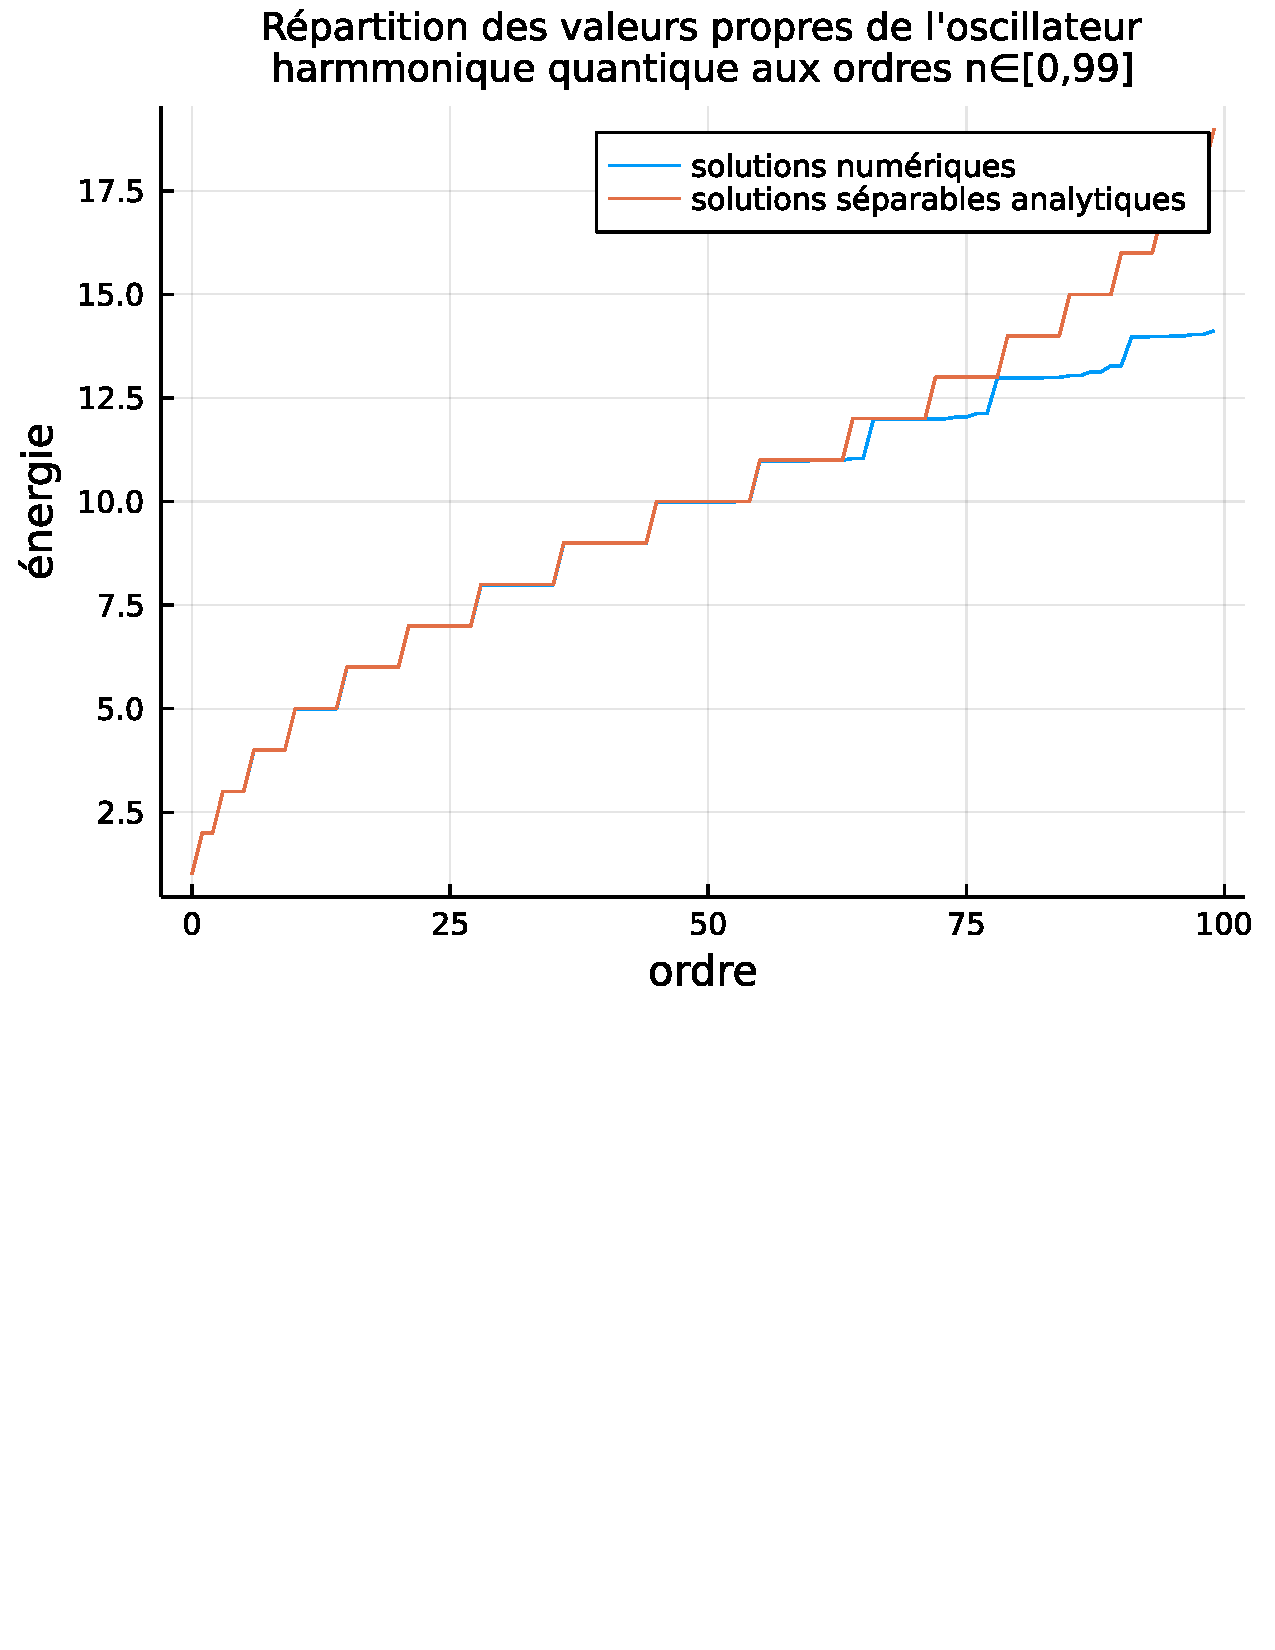
\includegraphics[width=.6\textwidth]{images/formes_résol_OHQ_2D/énergies_osc_harm2D_div.pdf}
    \caption{Énergies analytiques et numériques pour le hamiltonien de l'oscillateur harmonique 2D: numériques (différences finies) et analytiques.}
    \label{fig:en_lap_2D}
\end{figure}




 
Il existe plusieurs stratégies pour approcher numériquement des solutions d'EDP où les variables de temps et d'espace sont séparables. Les chimistes utilisent en général la méthode de \textsc{Rayleigh-Ritz} qui consiste, comme en mécanique, à \og projeter \fg{}\footnote{Léger abus de langage: il s'agit plutôt en fait de décomposer un ensemble de composantes que l'on choisit, et on appelle cela une base.} une solution sur une \og base \fg{}\footnote{Même remarque.} de fonctions dans le but de trouver la solution qui satisfait les équations du problème avec les conditions aux limites ou conditions initiales. Cela donne lieu à beaucoup d'activité de recherche sur l'optimisation de bases (notamment, gaussiennes), et j'ai pu discuter au travers du stage avec des chercheurs ou doctorants qui orientent leur recherche dans cette voie. 

Un autre moyen classique, est de discrétiser une partie de l'espace à l'aide de différences finies ou d'éléments finis. Dans mon cas, j'ai utilisé les différences finies pour le problème unidimensionnel physique (section \ref{sujet_stage})  et ferai néanmoins en sorte d'éviter d'avoir recours à une résolution 2D (ni en coordonnées d'espace ni en coordonnées généralisées) coûteuse en temps de calcul, mais je l'utiliserai pour avoir accès à une solution approchée de référence avec laquelle comparer les résultats. 






\begin{figure}[H]
    \centering
    \subfloat[\centering 25ème mode]{{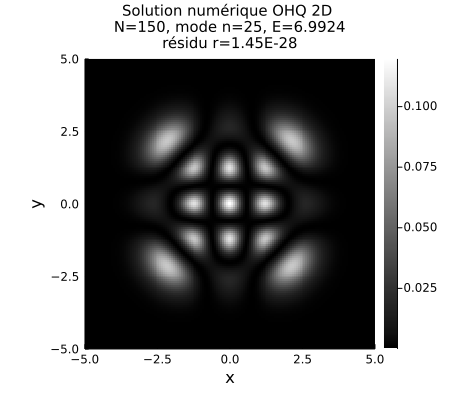
\includegraphics[width=.45\textwidth]{images/formes_résol_OHQ_2D/état_non_séparable.png} }}%
    \qquad
    \subfloat[\centering 26ème mode trouvé]{{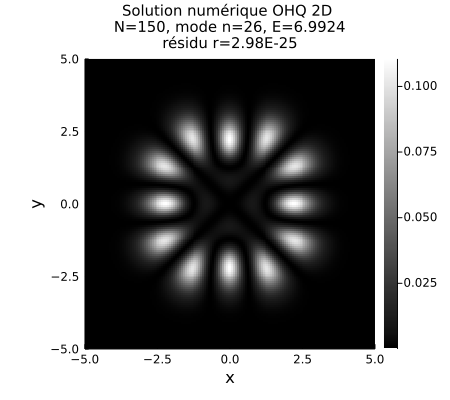
\includegraphics[width=.45\textwidth]{images/formes_résol_OHQ_2D/état_elliptique.png} }}%
    \caption[Exemples de cas séparables numériquement exhibés pour l'OHQ2D]{2 états non séparables qui ont convergé, trouvés par la résolution numérique avec laplacien à 5 points des valeurs propres de l'oscillateur harmonique quantique 2D avec $150 \times 150$ points sur la grille et le potentiel $V(x,y) = \frac{1}{2}(x^2+y^2)$, et les paramètres $m=\hbar = 1$. La résolution numérique utilise une méthode basée sur les espaces de \textsc{Krylov}.}%
    \label{fig:modes_non_separables}%
\end{figure}
Ce genre de résolutions numériques pose plusieurs problèmes qui peuvent influencer les résultats pour les plus grands modes:
\begin{itemize}
    \item D'abord, il y a bien-sûr l'erreur commise en raison de la discrétisation et le passage d'un problème dans $\mathcal{H}=L^2(\mathbb{R})$ espace hilbertien dans $\mathbb{R}^{N\times N}$ et  l'approximation des dérivées partielles par les différences finies. Typiquement, les valeurs propres les plus petites sont les mieux approchées pour la résolution du laplacien numérique à 5 points en 2D (ou à 3 points en 1D), et on peut prouver que n'importe quelle valeur propre du spectre du laplacien continu peut être approchée en discrétisant ainsi l'espace suffisamment finement. Mais qu'en est-il lorsque l'on a un hamiltonien  avec potentiel de confinement quelconque ? En illustration, la figure  \ref{fig:en_lap_2D} montre les énergies calculées numériquement des 100 premiers modes de l'oscillateur harmonique quantique 2D avec 100 points de discrétisation d'espace, et les valeurs théoriques associées aux modes propres séparables. On voit sur ce exemple que les plus petites énergies sont correctement approchées, mais que la divergence survient soudainement. La plupart du temps, mes expériences ont montré que les solutions séparables qu'on connaît sont trouvées pour les petites énergies seulement.  Mais la résolution aboutit à des solutions numériques non séparables plus \og exotiques \fg{} pour les grandes valeurs propres (figure \ref{fig:modes_non_separables}).

    \item Ensuite, un schéma à taille fixée ne permet pas de rendre compte des états liés de plus grande énergie, dont la fonction d'onde prend des valeurs significatives en dehors des frontières (tyipquement, au-delà de la précision machine), car l'ensemble de point satisfait nécessairement la condition de normalisation et la réalité physique n'est alors plus suffisamment bien approchée.
    
    
    \item Augmenter la précision requiert d'augmenter le nombre de points de discrétisation, ce qui a pour effet d'augmenter les temps de calcul ou l'instabilité numérique si le conditionnement devient mauvais, au risque de devoir recourir à des méthodes itératives dont la solution de départ peut influencer les solutions obtenues. En général, les vecteurs propres trouvés restent dépendants de l'algorithme de résolution, du bruit numérique, la forme du domaine, des effets d'échantillonnage, etc.
\end{itemize}

De la même manière, calculer un échantillonnage d'une solution séparable analytiquement exacte  connue pose ses propres problèmes. Pour reprendre l'exemple canonique de l'oscillateur harmonique, les formules analytiques comportent dans les formules des facteurs difficiles à calculer (en $\mathcal{O}(2^nn!)$ dans le cas des polynômes de \textsc{Hermite}), ce qui peut provoquer une instabilité numérique, lorsque des termes grands ou facteurs grands se compensent pour donner de petites quantités.  De plus, l'échantillonnage pose aussi ses propres problèmes, on obtient par exemple un repliement de spectre dans le calcul des intégrales de recouvrement approchées (c'est-à-dire, des produits scalaires des vecteurs-états entre eux) pour la solution exacte (figure \ref{fig:damier}). La conséquence est que certains modes ne sont pas orthogonaux entre eux à un seuil suffisant (seulement à $\approx 10^{-3}$ près pour les pires combinaisons, ce qui eat beaucoup). Cela peut poser problème pour d'éventuels calculs qui exploitent massivement l'hypothèse d'orthogonalité des modes, comme c'est le cas pour la théorie des perturbations.




\begin{figure}[H]
    \centering
    \subfloat[\centering modes analytiques échantillonnés]{{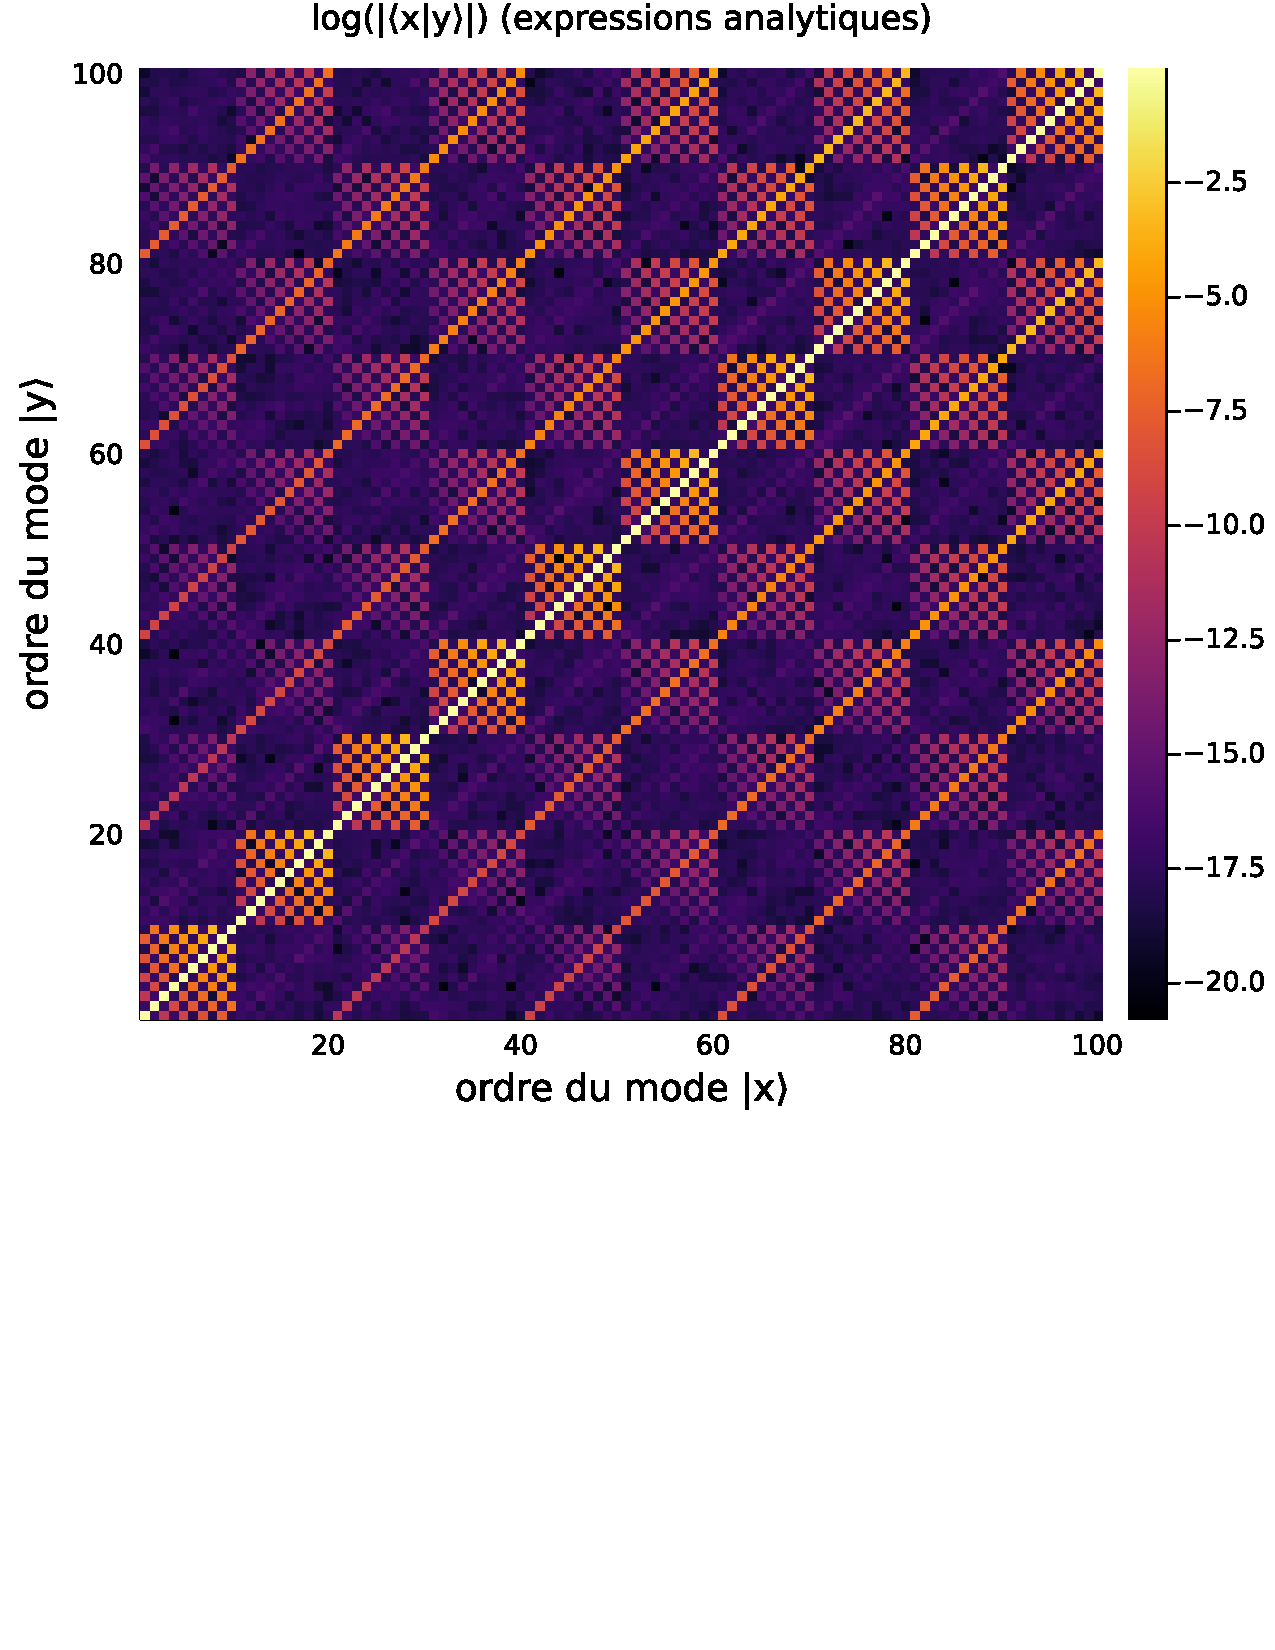
\includegraphics[width=.45\textwidth]{images/formes_résol_OHQ_2D/échecs.pdf} }}%
    \qquad
    \subfloat[\centering modes numériques]{{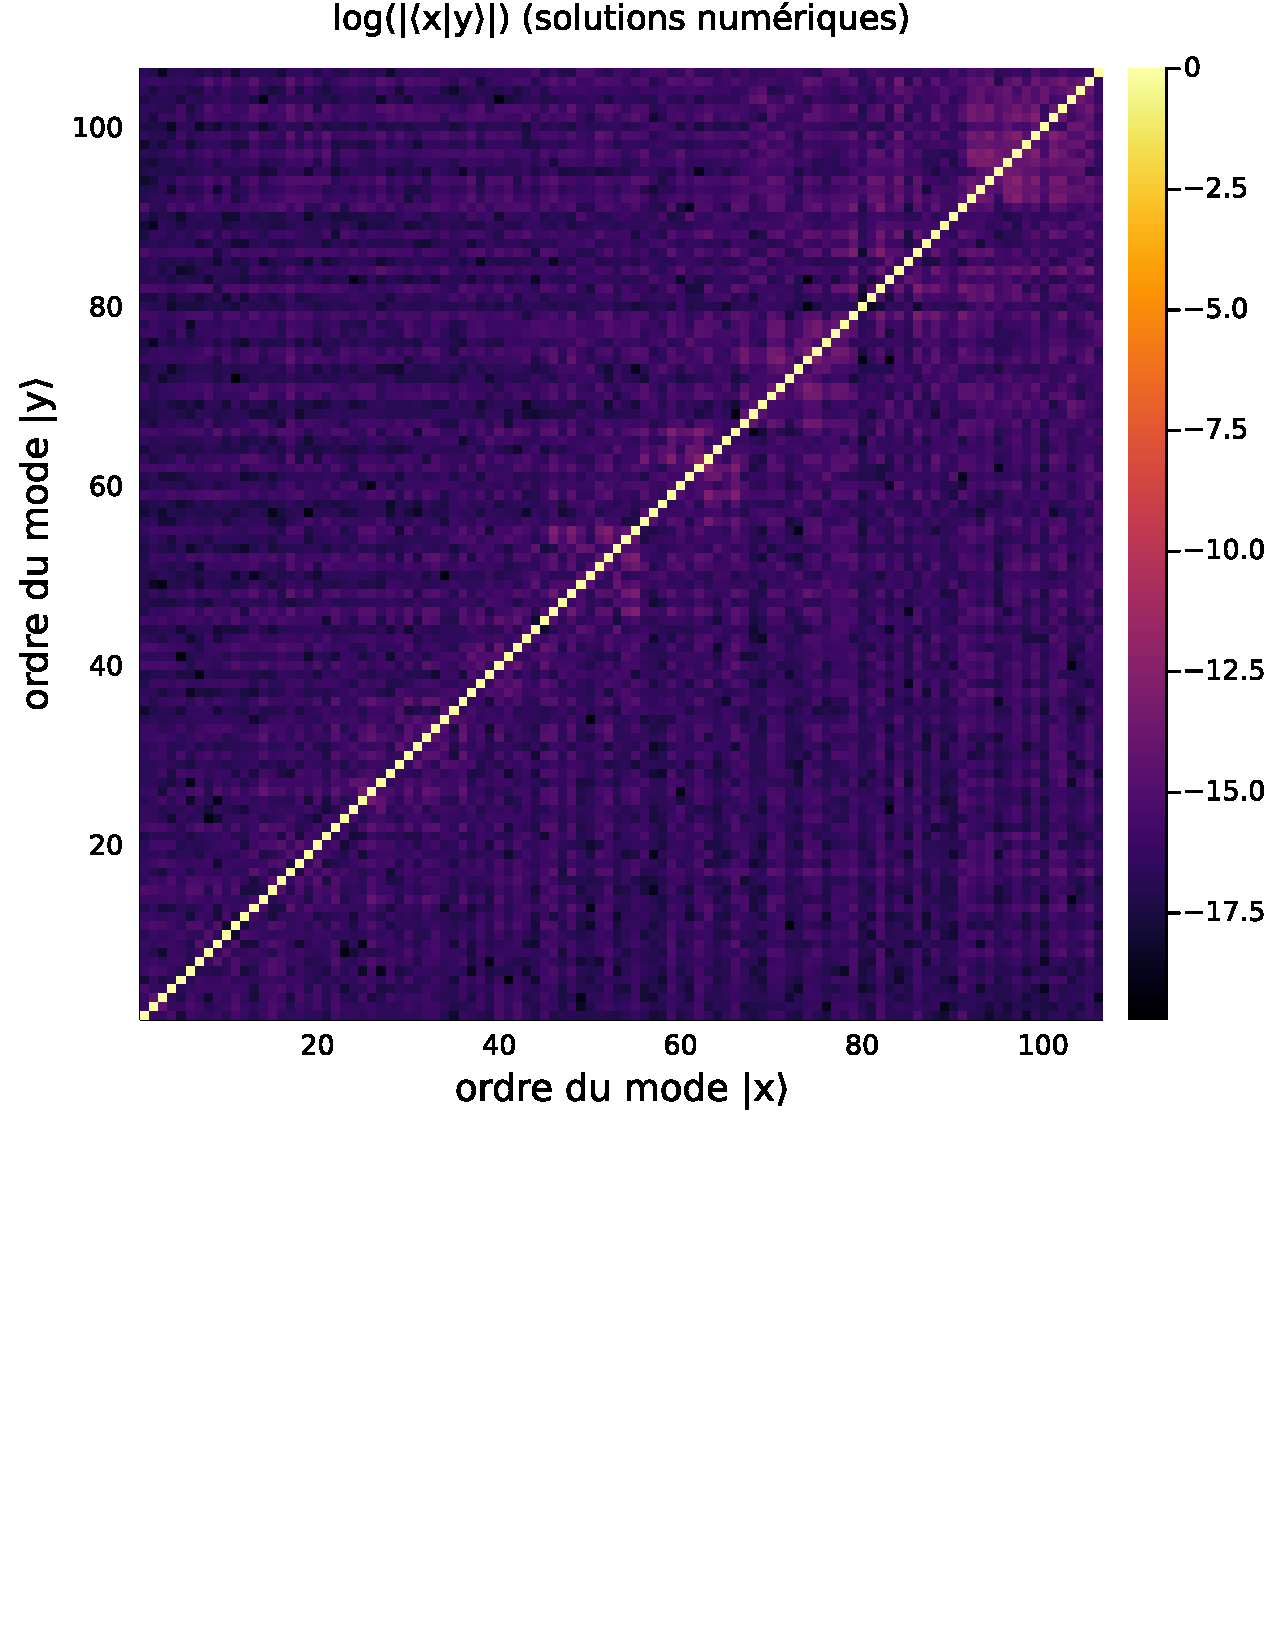
\includegraphics[width=.45\textwidth]{images/formes_résol_OHQ_2D/échecs_num.pdf} }}%
    \caption[Mesure de l'orthogonalité des modes analytiques et numériques]{Carte des produits scalaires entre les 100 premiers vecteurs propres séparables c'est-à-dire 10 modes possibles suivant chaque axe) échantillonnés d'après les formules analytiques et les vecteurs numériques trouvés, sur 150 points de discrétisation. On observe un repliement de spectre qui conduit à une mauvaise orthogonalité de certains modes entre eux. Pour des problèmes où l'orthogonalité est importante (comme la \textit{sum over states} en théorie des perturbations), le choix de l'arbitrage entre les deux ensembles de vecteurs se pose, en parallèle de la précision sur les énergies associées (figure \ref{fig:en_lap_2D}).}%
    \label{fig:damier}%
\end{figure}



\subsection{Généralités élémentaire et succinctes sur les problèmes d'analyse numérique les plus courants utilisés dans le contexte de ce stage}
\label{generalites_elt_analyse_num}
\subsubsection{Problèmes matriciels rencontrés}
En analyse numérique, on peut citer en particulier deux problèmes canoniques fondamentaux, qui sont immensément utiles en physique, ingénierie entre autres:
\begin{itemize}
    \item Résoudre un système linéaire: apparaît dans un nombre incalculable d'applications en général. En physique et en EDP, on peut citer: dans la simulation d'une EDP dans le temps avec un schéma implicite (comme \textsc{Crank-Nicholson}).
    
    \item Résoudre un problème aux valeurs propres ou un problème aux valeurs propres généralisées pour une matrice (comme pour \textsc{Schrödinger} stationnaire).
\end{itemize}

\paragraph{Sources d'erreur}
On distingue également quel que soit le problème deux sources d'erreurs qui contribuent:
\begin{itemize}
    \item \textbf{L'erreur d'arrondi}, due à la représentation discrète des nombres en machine;
    \item \textbf{L'erreur de troncature}, due à l'arrêt en temps fini de méthodes itératives, ou à la troncature de sommes, etc.
\end{itemize}

Dans les deux cas, le choix optimal de la méthode dépend beaucoup du type de matrice que l'on a en présence. La matrice est-elle creuse ? réelle ? complexe ? hermitienne ? tridiagonale ? triangulaire ? une combinaison de ces derniers ? etc. Ce sont autant de cas pour lesquels l'usage d'algorithmes dédiés donneront des résultats bien plus rapides en coût de calcul et garantissant une meilleure stabilité numérique. 



\subsubsection{Algorithmes courants pour la résolution de systèmes linéaires}

Pour résoudre des systèmes linéaires ou calculer une inverse, on connaît bien le pivot de \textsc{Gauss} dans le cas général, et les questions de stabilité numériques peuvent être plus ou moins garanties dans l'algorithme (en choisissant un pivot de plus grande valeur absolue possible, par exemple), ainsi que par des résultats analytiques, avec le conditionnement. Néanmoins, son coût de calcul est élevé, en $\mathcal{O}(n^3)$ pour une matrice $n\times n$.

D'autres algorithmes itératifs existent et présentent un compromis bien meilleur entre efficacité (vitesse de convergence) et précision, parmi lesquels on peut citer:
\begin{itemize}
    \item Méthode de \textsc{Gauss-Seidel}
    \item Méthode de \textsc{Jacobi} % (voir poly de MDI210)
\end{itemize}

On peut également passer par des décompositions, dont on connaît des algorithmes efficaces pour les calculer. Ensuite, on utilise des algorithmes  pour résoudre des systèmes linéaires à partir de la décomposition une fois acquise.

Une décomposition, pour une matrice $A$, est une factorisation ou un changement de base, qui exprime la matrice sous une forme aux propriétés intéressantes, ou plus explicites, plus facilement interprétables, plus stables numériquement, etc. On peut citer:
\begin{itemize}
    %\item Décomposition de \textsc{Dunford} (produit d'une diagonale et d'une nilpotente qui commutent)
    %\item Décomposition polaire (produit d'une orthogonale et d'une  hermitienne, analogue en toute dimension de l'écriture polaire d'un nombre  complexe)
    \item Factorisation de \textsc{Bunch-Kaufman} pour une matrice symétrique quelconque complexe (écrire $PAP^\intercal=LDL^\intercal$ où $P$ set une matrice de permutation, $L$ une triangulaire inférieure et  $D$ diagonale par blocs $1\times 1$ e t $2\times 2$)
    \item Factorisation de \textsc{Cholesky} pour une matrice hermitienne (écrire $A=LL^\star$ produit d'une triangulaire inférieure $L$ à diagonale réelle et positive  et sa conjuguée transposée)
    \item Décomposition LU (écrire $A=LU$, produit d'une triangulaire inférieure $L$ et d'une triangulaire supérieure $U$)
    \item Décomposition QR (écrire $A=QR$, produit d'une orthogonale $Q$ et d'une triangulaire supérieure $R$)
    \item Décomposition de \textsc{Schur} (écrire $PA=QUQ^{-1}=QUQ^\star$ changement de base orthogonal $Q$ vers une triangulaire supérieure $U$)
\end{itemize}

Certaines décompositions sont plus avantageuses que d'autres suivant le problème. Se ramener à des matrices triangulaires est en particulier très intéressant pour résoudre un système linéaire, car on peut directement trouver les inconnues récursivement en descendant ou remontant les lignes d'équations, et cela permet d'éviter de recourir au pivot de \textsc{Gauss} plus coûteux. 
Par exemple, orsque l'on a une matrice  hermitienne (très pertinent au regard des opérateurs hermitiens rencontrés en physique quantique), la décomposition de \textsc{Cholesky} est environ deux fois plus efficace que la décomposition LU\footnote{William H.; Saul A. Teukolsky; William T. Vetterling; Brian P. Flannery (1992). Numerical Recipes in C: The Art of Scientific Computing (second ed.). Cambridge University England EPress. p. 994.}.

\subsubsection{Algorithmes courants pour extraire des éléments propres}
Pour trouver des éléments propres analytiquement, en général on calcule d'abord le polynôme caractéristique, de trouver ses racines, puis on résoud un système linéaire dans un second temps.

Pour des matrices spéciales (par exemple, pour les matrices de \textsc{Toeplitz}, les matrices tridiagonales, les matrices de \textsc{Vandermonde}, etc), on peut parfois trouver par récurrence permet des formes closes ce qui permet d'aboutir à des résultats généraux. Il n'en est rien dans le cas général.



En général, appliquer ceci numériquement est une mauvaise idée. Plus précisément, tenter de calculer le polynôme caractéristique d'une matrice numériquement est en général une mauvaise idée, d'une part parce que l'opération est coûteuse\footnote{Il faut calculer $n!$ produits de termes}, et d'autre part parce qu'on ne connaît pas de formule générale pour la résolution de polynômes de degré supérieur ou égal à 5 (théorème d'\textsc{Abel-Rufini}), et enfin de petites erreurs sur le calcul des coefficients peuvent amener à de grandes erreurs sur les valeurs propres trouvée.




Lorsque l'on veut calculer numériquement des valeurs propres, il est raisonnable de classer les solveurs propres en fonction de la taille et de la configuration non nulle de la matrice. Numériquement, trouver des valeurs propres nécessitent un processus itératif parmi lesquels on peut citer:

\begin{itemize}
    \item Méthodes de la puissance itérée
    \item Méthodes d'\textsc{Arnoldi}, basées sur la construction de sous-espaces de \textsc{Krylov}  % (voir Numerical Methods for large eigenvalue problems)
    %\item Méthode des gradients conjugués % [voir \cite{poliak_introduction_1987}]
\end{itemize}

À titre d'exemples, voici en annexes \ref{ann:rech_elts_propres} quelques résultats  sur la localisation de spectres et les méthodes de la puissance que j'ai eu l'occasion de rencontrer durant ma scolarité, dans les cours de l'École Centrale de Lyon ou ailleurs qui portent sur l'obtention itérative d'élements propres.

Pour obtenir rapidement et de manière fiable des états propres cependant, j'utiliserai les codes éprouvés des nombreuses bibliothèques disponibles en Julia, en particulier \codewordred{KrylovKit}, qui renvoie également des métadonnées sur le succès de convergence, les résidus, etc. à chaque appel de la fonction. Je ne m'attarderai pas davantage dans ce rapport (ni l'ai-je fait pendant le stage) sur les mathématiques sous-jacentes de ces algorithmes connus, car ce n'est pas vraiment l'objet. Il faut simplement se rappeler que ces méthodes sont itératives en appliquant la fonction linéaire un grand nombre de fois, et qu'elles construisent des bases orthogonales de sous-espaces, et donc qu'elles sont coûteuses en temps et en espace. Il convient de minimiser leurs appels, et de minimiser la dimension de \textsc{Krylov} choisie et la dimension des arguments.




\subsubsection{Contrôle d'erreur a posteriori}



Une fois que l'on dispose numériquement de vecteurs propres ou valeurs propres, il peut être intéressant, voire il est absolument nécessaire, de pouvoir contrôler l'erreur commise. 




Pour connaître l'influence d'une perturbation sur les éléments propres d'une matrice, que ce soit des perturbations souhaitées (modification du hamiltonien dans la théorie des perturbations) ou non souhaitées (comme une erreur de troncature).



\begin{theorem}{(Corollaire 3.3, \cite{saad_numerical_2011})}
    SI $A$ est une matrice hermitienne, $\tilde{\lambda}$ une valeur propre approchée et $\tilde{u}$ son vecteur propre approché, et $r=A\tilde{u} - \tilde{\lambda} \tilde{u}$, alors il existe une valeur propre $\lambda$ de $A$ telle que \begin{equation}
        |\lambda - \tilde{\lambda} | \le \|r\|_2
    \end{equation}
\end{theorem}


Enfin, nous avons l'inégalité de \textsc{Kato-Temple} qui porte sur un opérateur pas forcément en dimension finie, et donne un résultat fort, très utilisé dans le contexte de la mécanique quantique pour évaluer la précision d'états propres approchés d'opérateurs.


\begin{theorem}{(\textsc{Kato-Temple})}
Soit $\mathcal{H}$ un espace de \textsc{Hilbert} et $A$ un opérateur auto-adjoint de $A$. Soit $\tilde{u}$ un vecteur propre approximatif normé de $A$ et  $\tilde{\lambda} = \langle A\tilde{u}|\tilde{u}\rangle$ sa valeur propre approchée. On définit $r$ le résidu $r=A\tilde{u}-\tilde{\lambda} \tilde{u}$ et  $\varepsilon = \|r\|$ la norme du résidu. Soit $]\alpha,\beta[$ un intervalle  contenant $\tilde{\lambda}$. Si le seul point du spectre de $A$ est $\lambda$, alors on a l'inégalité
\begin{equation}
\label{kato_temple_inqeuality}
    - \frac{\varepsilon^2}{\beta - \tilde{\lambda}} \le \lambda - \tilde{\lambda} \le \frac{\varepsilon^2}{\tilde{\lambda} - \alpha}
\end{equation}
\end{theorem}






\subsection{Simulations numériques: présentation des méthodes \emph{hardware et software}}

Pour simuler numériquement les équations de \textsc{Schrödinger} stationnaires, j'ai eu recours eu langage JULIA qui m'a été proposé, que j'ai appris pour l'occasion, et qui faisait donc partie du travail compris dans le stage.




\subsubsection{Présentation rapide de JULIA}
Julia est un langage jeune, typé dynamiquement (c'est-à-dire que les variables peuvent changer de type), de haut niveau  (c'est-à-dire, proche du langage humain), performant. La syntaxe est proche du python, mais contrairement à ce dernier, Julia est un langage compilé, et son efficacité et sa rapidité est proche de celles du C, ce qui en fait un langage de premier choix pour le calcul scientifique car il combine ces deux avantages, ce qui est remarquable.

Pour les besoins des simulations j'ai eu l'occasion de travailler avec beaucoup de bibliothèques orientées calcul scientifique. Cela a été pour moi l'occasion de travailler sur les bonnes pratiques d'état de l'art en simulation numérique et sur l'optimisation\footnote{Par \og optimisation \fg{} j'entends: parvenir à la solution donnée avec la précision requise en résuisant au maximum les ressources (en calcul, en temps) utilisées.} du code.
\begin{itemize}
    \item \codewordred{BenchmarkTools}, \codewordred{Profile} (pour l'évaluation des performances du code)
    \item \codewordred{SparseArrays}, \codewordred{LinearAlgebra}, \codewordred{SpecialMatrices}, pour la manipulation des tableaux;
    \item \codewordred{DSP}, \codewordred{ImageFiltering}, \codewordred{FFTW}  pour la transformée de \textsc{Fourier} rapide et la manipulation de noyaux de convolution (qui ont servi notamment pour étudier Julia au début sur des codes de propagation de paquets d'ondes, et obtenir des dérivées fréquentielles);
    \item \codewordred{KrylovKit}, \codewordred{IterativeSolvers}, \codewordred{LinearMaps}, \codewordred{LinearOperators} pour les algorithmes itératifs (\textsc{Arnoldi}, \textsc{Krylov}, gradients conjugués, etc), pour algorithmes itératifs; \codewordred{Arpack}\footnote{Ce n'est pas une bibliothèque Julia à proprement parler mais une interface pour les \href{https://www.caam.rice.edu/software/ARPACK/}{routines} Fortran 77 de résolution de problèmes aux valeurs propres en grande dimension.} pour résoudre des problèmes aux valeurs propres;
    \item \codewordred{Polynomials}, \codewordred{SpecialPolynomials} pour la manipulation des polynômes de Hermite notamment.
    \item \codewordred{CUDA} et ses sous-librairies \codewordblue{CUDA.CUSPARSE}, \codewordblue{CUDA.CUSOLVER}, \codewordblue{CUDA.CUFFT}, qui transcendent les paquets précédents (par exemple les méthodes itératives de \codewordred{KrylovKit} et \codewordred{IterativeSolvers}  évoquées fonctionnent avec des vecteurs CUDA, on peut donc faire tourner leurs routines sur le processeur graphique, au prix d'une précisions simple au lieu de double sur des GPU grand public).
    \item \codewordred{Graphs},  \codewordred{DataStructures}, \codewordred{MetaGraphsNext} pour l'utilisation de graphes étendus (dont les arêtes et sommets peuvent être surchargés par des \textit{types composites} pour résoudre un problème personnalisé) dans la partie programmation dynamique pour optimiser les stratégies de calcul.
\end{itemize}

J'aurai l'occasion de revenir plus en détail sur l'usage de JULIA dans le cadre du problème qui nous intéresse.



Comme déjà évoqué, JULIA est un langage en devenir mais qui manque encore de documentation. J'ai pu m'en rendre compte lors de mes lectures de documentation, au travers des forums de développement. On y trouve encore l'évocation de bugs à améliorer, de fonctions à ajouter, de typages à corriger, etc. Un travail de fond important a alors consisté à tester les algorithmes sur des cas représentatifs pour voir lesquels étaient les plus rapides, car au delà des mathématiques qui fondent l'\textit{algorithme}, le \textit{programme} peut montrer des performances légèrement différentes selon le type de machine, la parallélisation, son matériel, etc.  % D'autre part, tandis que JULIA possède une API vers quelques fonctions de LAPACK, mais pas toutes, et le manque de documentation est assumé, comme on peut le lire \href{https://docs.julialang.org/en/v1/stdlib/LinearAlgebra/#LAPACK-functions}{ici}. Je reviendrai sur ces détails ultérieurement.





% parler de l'arbitrage entre sparse + krylov VS les types hermitian ou Symtridiagonal en fonction du nombre de valeurs propres voulues, mais l'inconvénient de l'automatisation du choix du nombre de dimensions de Krylov
%parler de Bunch-Kaufman
%Parler de LAPACK, des Computational Routines for Eigenvalue Problems, de CUDA avec CUDA Toolkit Documentation

%Parler de LAPACK et de sa \href{https://www.netlib.org/lapack/lug/node24.html}{nomenclature} et ses \href{http://sites.science.oregonstate.edu/~landaur/nacphy/lapack/eigen.html}{Computational Routines for Eigenvalues Problems}
%BLAS vs MKL ??


\paragraph{Parallélisation sur GPU: généralités}
\label{parallelisation_GPU}

En sus de l'ensemble des algorithmes existants pour tel ou tel problème, certains sont hautement parallélisables, on peut alors les exécuter sur des GPU (\textit{Graphic Processor Unit}), destinés à leur invention à calculer des transformations géométriques de triangles pour l'affichage de graphiques, ils se sont rapidement avérés particulièrement utiles aux informaticiens pour l'algèbre linéaire et le Machine Learning en particulier. Parec qu'un processeur graphique dispose de très grandes quantités de c\oe{}urs, il accélère considérablement des calculs en les exécutant en même temps\footnote{\url{https://docs.nvidia.com/cuda/cuda-c-programming-guide/index.html#from-graphics-processing-to-general-purpose-parallel-computing}}, alors qu'ils devraient être exécutés les uns après les autres sur un c\oe{}ur de processeur classique. Nvidia fournit des API pour ses processeurs au travers de la bibliothèque CUDA (pour \textit{Compute Unified Device Architecture}), avec des interfaces dans de nombreux langages sont C++ et JULIA, particulièrement \href{https://docs.nvidia.com/cuda/cusolver/index.html}{CUSOLVER}. On trouve de nombreux examples de \emph{wrappers} en Julia sur \href{https://github.com/JuliaGPU/CUDA.jl}{Github}.



Il est à noter que dans bien des cas, l'usage des fonctions sur CPU reste le plus efficace, plus rapide, et très bien optimisé par les compilateurs efficaces (en Julia, qui est amplement conçu pour le calcul scientifique, c'est le cas).

Cela s'explique par les temps de transit entre la mémoire du GPU et celle du CPU, qui dépassent généralement les temps de calcul pour des opérations sur des données de petite taille. En effet, le GPU était un processeur à part entière, il n'est pas synchronisé avec le CPU. Des temps d'attente peuvent aussi empirer les performances du code. En ce sens, \textbf{le calcul sur GPU se révèle en général très utile pour certains problèmes pouvant mettre en \oe{}uvre massivement et répétitivement des calculs matriciels lourds mais son recours n'est absolument pas systématique. Le calcul à haute performance} (ou HPC pour \textit{High-Performance Computing}), qui est une discipline de l'informatique, s'attache à exploiter intelligemment au mieux le potentiel des GPU surtout pour des problèmes à grande échelle, en faisant un meilleur usage du matériel (cache, etc) y compris à bas niveau (proche de la machine) qui peuvent se révéler utile dans mon sujet de stage\footnote{Précisément, on m'a expliqué que contrôler mieux l'utilisation du cache dans les GPUs permet d'optimiser des calculs. Ça aurait par exemple pu être utile pour faire des produits creux d'un hamiltonien par un état avec un simple décalage des lignes entre elles, comme me l'a suggéré Paul Cazeaux.}. J'ai eu l'occasion de discuter sur ce point avec des chercheurs du Laboratoire de Chimie Théorique (LCT) de Sorbonne Université lors d'un séminaire organisé pendant mon stage, quoique cela ne fît absolument pas partie de mon travail.


En annexe \ref{algos_vp_ex_num}, j'ai mis un exemple très concret de calcul d'éléments propres pour le cas de la matrice du laplacien à 5 points dont on connaît les valeurs et vecteurs propres analytiquement, pour démontrer les avantages et inconvénients des deux paradigmes (GPU et CPU).

En annexe \ref{sec:optim_hardware}, j'ai décrit tout un travail annexe réalisé pendant ce stage, qui repose sur l'idée d'alterner entre CPU et GPU pour certains calculs lourds dans un algorithme calculatoire, tout en choisissant un chemin minimisant le temps machine utilisé. Il s'agit pour l'heure seulement d'une heuristique, car la complexité combinatoire derrière le problème est prohibitive. Je n'ai finalement pas utilisé l'algorithme de décision réalisé car comme je le décris plus bas dans ce rapport, les étapes délicates qui prennent le plus de temps (à savoir le calcul de la référence pour l'état, ce qu'on s'interdit normalement de faire) est plus précis et rapide sur mon CPU (machine grand public).

\chapter{Partie centrale du stage: simulation numérique d'équations de \textsc{Schrödinger}}

Cette section porte cette fois sur le travail qui constitue le sujet de mon stage exposé linéairement. Je conçois les algorithmes nécessaires au fur et à mesure et j'applique les théorèmes connus des chapitres précédents pour parvenir à des résultats intéressants.


\section{Définition du problème}
\label{sujet_stage}

Le sujet de ce stage s'intéresse à un système de trois particules dont l'une est beaucoup plus massive que les deux autres, lesquelles vivent sur un axe, en 1D.

Ce cas est fortement inspiré de l'ion $H_2^+$ (deux protons massifs de  masses identiques $m_p$ et un électron de masse $m_e$ gravitant autour d'eux évoluant sur une droite). Les tests numériques seront d'ailleurs effectués pour cet ion.

On part du hamiltonien en coordonnées généralisées 1D: nous avons 3 particules évoluant en 1D donc 3 dimensions a priori:
\begin{equation}
    \mathcal{H}(X_1,X_2,x, \vect{P}_1,\vect{P}_2,\vect{p}) = \frac{\vect{P}_1^2}{2M_1} + \frac{\vect{P}_2^2}{2M_2} + \frac{\vect{p}^2}{2m} + \mathcal{V}_1(x-X_1) + \mathcal{V}_2(x-X_2) + \mathcal{W}(X_2-X_1)
\end{equation}

En physique classique, on peut alors exprimer les quantités de mouvement en fonction des variables de position.

Le but ultime étant de trouver la configuration de l'état fondamental (de plus basse énergie).


\section{Changement de coordonnées et réduction des DDL}



Pour simplifier le problème, on va supposer que le système est isolé, la position du centre de masse ne nous intéresse alors pas.

Nous allons alors effectuer le changement de coordonnées $(X_1,X_2,x) \rightsquigarrow (X_G, R, r)$, avec $X_G$ le barycentre de masse des trois particules:

\begin{equation}
    X_G = \frac{M_1 X_1 + M_2 X_2 + mx}{M_1 + M_1 + m }
\end{equation}
et $R$ la distance séparant algébrique les deux noyaux, et $r$ la distance algébrique de l'électron au centre de masse. En figure \ref{fig:chgt_coord}, sont représentés ces paramètres.


\begin{figure}[H]
    \centering
    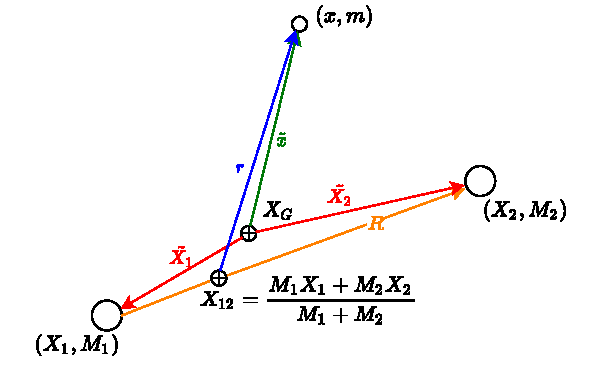
\includegraphics{images/changement_coordonnées.pdf}
    \caption[Paramétrage et notations pour  le changement de coordonnées]{Les deux paramétrages et les relations entre les paramètres. Le dessin \og déplié \fg{} dans le plan 2D sert uniquement à la lisibilité. Les trois particules restent alignées, sur un unique axe.}
    \label{fig:chgt_coord}
\end{figure}

Nous avons donc

\begin{equation}
\begin{bmatrix}
X_G \\[3pt]
r \\[3pt]
R \\[3pt]
\end{bmatrix}
= 
\begin{bmatrix}
\frac{M_{1}}{M_{1} + M_{2} + m} & \frac{M_{2}}{M_{1} + M_{2} + m} & \frac{m}{M_{1} + M_{2} + m} \\
-\frac{M_{1}}{M_{1} + M_{2}} & -\frac{M_{2}}{M_{1} + M_{2}} & 1 \\
-1 & 1 & 0
\end{bmatrix} \times 
\begin{bmatrix}
X_1 \\[3pt]
X_2 \\[3pt]
x \\[3pt]
\end{bmatrix}
\end{equation}
Ce système est bien un changement de coordonnées inversible, car son déterminant vaut
\begin{equation}
    \newcommand{\Bold}[1]{\mathbf{#1}}-\frac{M_{1}}{M_{1} + M_{2} + m} - \frac{M_{2}}{M_{1} + M_{2} + m} - \frac{M_{1} m}{{\left(M_{1} + M_{2} + m\right)} {\left(M_{1} + M_{2}\right)}} - \frac{M_{2} m}{{\left(M_{1} + M_{2} + m\right)} {\left(M_{1} + M_{2}\right)}} <0
\end{equation}
Dans un souci d'efficacité et de reproductibilité on inverse symboliquement le système par le calcul formel avec \href{www.sagemath.org/}{SageMath}:


\begin{minted}[
frame=lines,
framesep=2mm,
baselinestretch=1,
fontsize=\small,
breaklines=true,
linenos=false,
bgcolor=white,
escapeinside=||,
mathescape=true]{python}
X_1, X_2, x, M_1, M_2, m = var('X_1, X_2, x, M_1, M_2, m')
M = matrix(SR, 3, 3,
    [M_1/(M_1+M_2+m), M_2/(M_1+M_2+m), m/(M_1+M_2+m),
    -M_1/(M_1+M_2), -M_2/(M_1+M_2), 1,
    -1, 1, 0]) # création matrice conversion $(X_1,X_2,x)$ vers $(X_G,r,R)$
inv(M) 
\end{minted}

de là on déduit
\begin{equation}
\begin{bmatrix}
X_1 \\[3pt]
X_2 \\[3pt]
x \\[3pt]
\end{bmatrix}
=
\left(\begin{array}{rrr}
1 & -\frac{m}{M_{1} + M_{2} + m} & -\frac{M_{2}}{M_{1} + M_{2}} \\
1 & -\frac{m}{M_{1} + M_{2} + m} & \frac{M_{1}}{M_{1} + M_{2}} \\
1 & \frac{M_{1} + M_{2}}{M_{1} + M_{2} + m} & 0
\end{array}\right)
\times
\begin{bmatrix}
X_G \\[3pt]
r \\[3pt]
R \\[3pt]
\end{bmatrix}
\end{equation}

On peut ensuite expliciter les anciennes coordonnées en fonction des nouvelles:
\begin{minted}[
frame=lines,
framesep=2mm,
baselinestretch=1,
fontsize=\small,
breaklines=true,
linenos=false,
bgcolor=white,
escapeinside=||,
mathescape=true]{python}
nv_coord = matrix(SR, 3,1, var('X_G, r, R')) # nouveau paramétrage
an_coord = inv(M)*nv_coord
X_1 = an_coord[0,0].factor()
X_2 = an_coord[1,0].factor()
x   = an_coord[2,0].factor()
\end{minted}

Avec les variables ainsi exprimées, on trouve parallèlement

\begin{equation}
    \mathcal{V}_1 (x-X_1) = \mathcal{V}_1\left(\frac{M_{2} R + M_{1} r + M_{2} r}{M_{1} + M_{2}} \right)
\end{equation}
\begin{equation}
    \mathcal{V}_2 (x-X_2) = \mathcal{V}_2\left(-\frac{M_{1} R - M_{1} r - M_{2} r}{M_{1} + M_{2}} \right)
\end{equation}

et
\begin{equation}
    \mathcal{W}(X_2-X_1) = \mathcal{W}(R)
\end{equation}

enfin, en supposant que $\dot{X}_G=0$, puisque notre système est isolé (cette hypothèse physique sera justifiée dans la section suivante), on peut réévaluer la partie cinétique du hamiltonien (chaque variable portée par un  symbole arbitraire \codeword{v} en code ici désigne la quantité $\dot{v}$ en physique):

\begin{minted}[
frame=lines,
framesep=2mm,
baselinestretch=1,
fontsize=\small,
breaklines=true,
linenos=false,
bgcolor=white,
escapeinside=||,
mathescape=true]{python}
Ec(X_1, X_2, x) = 1/2*M_1*X_1^2 + 1/2*M_2*X_2^2 + 1/2*m*x^2
Ec(0, r, R) # système isolé
\end{minted}
qui permet d'écrire $\dot{X}_G = 0 \Rightarrow$
\begin{equation}
\label{en_cin_red}
    \frac{\vect{P}_1^2}{2M_1} + \frac{\vect{P}_2^2}{2M_2} + \frac{\vect{p}^2}{2m} = \frac{\left(M_{1}^{2} M_{2} + M_{1} M_{2}^{2} + M_{1} M_{2} m\right) \dot{R}^{2} + \left(M_{1}^{2} m + 2 \, M_{1} M_{2} m + M_{2}^{2} m\right) \dot{r}^{2}}{\left(M_{1} + M_{2} + m\right)\left(M_{1} + M_{2}\right)}
\end{equation}

Ainsi en posant en plus $X_G=0$, on peut réécrire le hamiltonien classique comme fonction de deux variables $r,R$ qui décrivent complètement l'état des trois particules avec $\mu_R$ et $\mu_r$ des \textbf{masses réduites} qui apparaissent dans l'équation \ref{en_cin_red}:
\begin{multline}
    \tilde{\mathcal{H}}(r, R, p, P) = \frac{1}{2\mu_R} P^2 + \frac{1}{2\mu_r} p^2 \\ + \underbrace{\mathcal{V}_1\left(\frac{M_{2} R + M_{1} r + M_{2} r}{M_{1} + M_{2}} \right) + \mathcal{V}_2\left(-\frac{M_{1} R - M_{1} r - M_{2} r}{M_{1} + M_{2}} \right)  + \mathcal{W}(R)}_{\mathcal{Y}(r,R)}
\end{multline}

où $(P,p)$ sont les variables conjuguées respectives de $(R,r)$, et $\mu_r$ et $\mu_R$ les masses réduites données par

\begin{equation}
    \boxed{\mu_R = \frac{M_{1}^{2} M_{2} + M_{1} M_{2}^{2} + M_{1} M_{2} m}{\left(M_{1} + M_{2} + m\right)\left(M_{1} + M_{2}\right)}}
\end{equation}
\begin{equation}
    \boxed{\mu_r = \frac{M_{1}^{2} m + 2 \, M_{1} M_{2} m + M_{2}^{2} m}{\left(M_{1} + M_{2} + m\right)\left(M_{1} + M_{2}\right)}}
\end{equation}

D'où l'équivalent quantifié du hamiltonien:
\begin{equation}
    \boxed{\tilde{H} = - \frac{1}{2\mu_R} \frac{\partial^2}{\partial R^2} - \frac{1}{2\mu_r} \frac{\partial^2}{\partial r^2} + \mathcal{Y}(r,R)}
\end{equation}




\section{Choix de fonctions numériques pour le hamiltonien de  l'ion $H_2^+$}
\label{sec:choix_fonctions}


Conformément aux sections précédentes et l'introduction du chapitre,  on désigne sur l'unique axe les variables-coordonnées scalaires généralisées
\begin{itemize}
    \item $r$ qui représente la coordonnée de l'électron par rapport au centre de masse;
    \item $R$ qui représente le rayon la molécule (distance séparant les deux noyaux).
\end{itemize}
Le référentiel barycentrique de la molécule est supposé galiléen car on suppose les noyaux non accélérés par des forces externes. On prend en compte  les énergies cinétiques des noyaux et de l'électron respectivement dans ce référentiel barycentrique, ainsi qu'un potentiel décrivant leur interaction, qui complique la résolution et empêche \emph{a priori} toute résolution à variables séparées. 

On prend donc le hamiltonien 1D non relativiste de 2 coordonnées généralisées $r$ et $R$ indépendant du temps. On pose  d'après le paragraphe précédent:
\begin{equation}
    M = \frac{2 m_p^3 + m_p^2m_e}{2(2m_p+m_e)m_p}
\end{equation}
et
\begin{equation}
    m = \frac{2 m_p^2m_e}{m_p(2m_p+m_e)}
\end{equation}
dans
\begin{equation}
\label{hamiltonien_original}
    \boxed{\hat{H} = \underbrace{-\frac{1}{2m} \frac{\partial^2}{\partial r^2}}_{\hat{T}_{\text{coord. él.}}} \quad \underbrace{-\frac{1}{2M} \frac{\partial^2}{\partial R^2}}_{\hat{T}_{\text{coord. nucl.}}} \quad + \underbrace{V(r,R)}_{\text{potentiel d'interaction}}}
\end{equation}

qui opère sur $L^2(\mathbb{R} \times \mathbb{R})$.

Pour notre étude, on prendra conventionnellement les potentiels d'interaction
\begin{equation}
    \mathcal{V}_{\text{noy.-él.}}^{(1)}(d_{\text{prot.-él.}}) = \mathcal{V}_{\text{noy.-él.}}^{(2)}(d_{\text{prot.-él.}}) = -V_0 \exp \left( - \frac{d_{\text{prot.-él.}}^2}{2\sigma^2}\right)
\end{equation}
qui représente un puits normalisé autour de chaque proton; ainsi que

\begin{equation}
    \mathcal{W}_{\text{prot.-prot.}}(d_{\text{prot.-prot.}}) =     \frac{\beta}{\sqrt{\eta^2 + d_{\text{prot.-prot.}}^2}}
\end{equation}
avec $\beta, \eta, V_0, \sigma$ des paramètres à fixer à l'avance empiriquement, qui représente un potentiel électrostatique en $\frac{1}{d_{\text{prot.-prot.}}}$ rectifié (pour ne pas avoir de singularité).

Avec nos choix de masses nucléaires identiques, on a donc
\begin{equation}
    V(r,R) = \mathcal{W}_{\text{prot.-prot.}} (R) + \mathcal{V}_{\text{noy.-él.}}\left( r+ \frac{R}{2}\right) + \mathcal{V}_{\text{noy.-él.}}\left( r- \frac{R}{2}\right) 
\end{equation}

\begin{equation}
\label{potentiel_H2plus}
    \boxed{V(r,R) = -V_0 \left[\exp \left( - \frac{(r-\frac{R}{2})^2}{2\sigma^2}\right) + \exp \left( - \frac{(r+\frac{R}{2})^2}{2\sigma^2}\right) \right] +  \frac{\beta}{\sqrt{\eta^2 + R^2}}}
\end{equation}

ou de manière plus compacte:
\begin{equation}
    V(r,R) = -2V_0 \exp \left( -\frac{1}{2\sigma ^2}\left(r^2+\frac{R^2}{4}\right) \right) \cosh (rR) +  \frac{\beta}{\sqrt{\eta^2 + R^2}}
\end{equation}


\subsection{Choix des paramètres}

\textbf{Pour la suite, je prendrai les paramètres $\beta=1.5, \eta=0.5, V_0 = 1.5, \sigma = 1$, $m_e = 1, m_p = 6$.} Cela permet d'avoir quelques états propres de valeur propre négative, et jouer sur les paramètres permettrait de piloter le spectre du hamiltonien associé au potentiel. Les figures de ce rapport sont générées avec ces paramètres de sorte que la carte du potentiel choisi est donnée en figure \ref{fig:potentiel_params_indiques}.

\begin{figure}
    \centering
    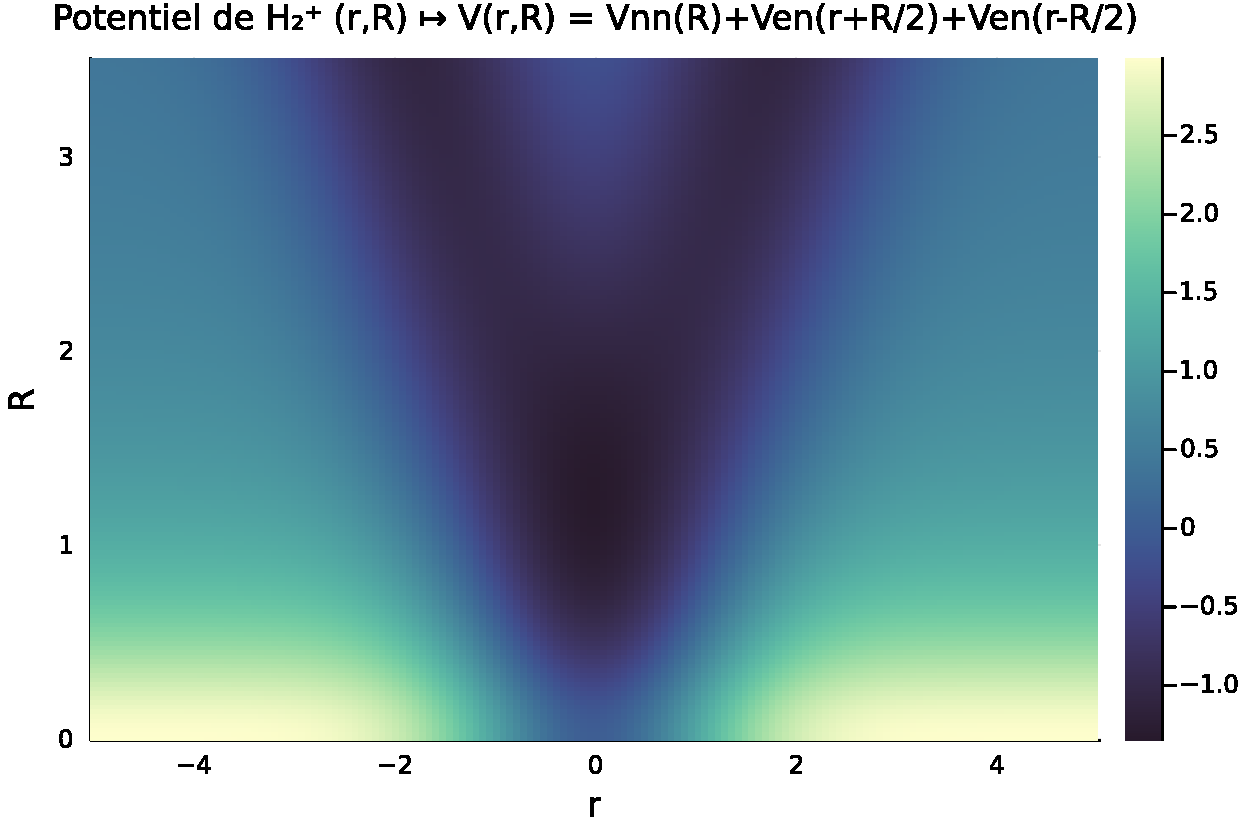
\includegraphics[width=.7\textwidth]{images/formes_résol_H2+/potentiel_original_R.pdf}
    \caption[Potentiel choisi pour la résolution avec les paramètres choisis de la modélisation]{Potentiel choisi pour la résolution avec les paramètres indiqués.  Physiquement on retrouve bien notre modélisation: à $R$ fixé, deux puits de potentiel sont visible selon l'axe des $r$, qui correspondent aux deux protons.}
    \label{fig:potentiel_params_indiques}
\end{figure}


\section{Séparation des termes et approximation de \textsc{Born-Oppenheimer}}
En règle générale, il est commode d'avoir un hamiltonien séparable, par exemple de la forme

\begin{equation}
    \hat{H} = \hat{H}_{\text{él.}} + \hat{T}_{\text{noy.}}
\end{equation}


Pour ce faire, on mettra en \oe{}uvre l'approximation de \textsc{Born-Oppenheimer} en découplant la dynamique noyau-électron du fait du grand rapport de masse entre l'électron et les noyaux. Les prémices de cette technique ont  été proposées en 1927 par les deux physiciens éponymes dans l'article intitulé \og Zur Quantentheorie der Molekln \fg{} (\textit{Sur la théorie quantique des molécules}) \cite{born_zur_1927}. L'hypothèse $m_p \gg m_e$ permet de supposer les noyaux fixes, ce qui permet de considérer $R$ comme un hyperparamètre de notre problème, que l'on trouve d'abord  en minimisant l'énergie fondamentale de la fonction d'onde de l'électron à $R$ fixé, qui est appelée \textbf{énergie potentielle de surface}\footnote{Dans des situations où la molécule comprend beaucoup d'atomes, cette énergie de surface est une fonction des paramètres géométriques de la molécule, et l'analogie avec une  \og surface \fg{}, ou un relief décrivant cette énergie en fonction de sa forme géométrique, donne sens à cette dénomination.}. Une énergie potentielle de surface  est usuellement définie comme l'énergie d'interaction d'une collection d'atomes fixes en configuration fixée donnée par des coordonnées d'espace généralisées. En chimie moléculaire il est utile de faire varier de manière infinitésimale ces coordonnées nucléaires (correspondant à $R$ dans notre cas) puis de trouver les valeurs propres du système ainsi simplifié par rapport aux électrons, pour obtenir cette \og carte \fg{} de l'énergie en fonction des positions nucléaires et obtenir ensuite la configuration la plus stable d'énergie minimale, car les propriétés de l'énergie de surface au voisinage de ce minimum régissent les spectres vibrationnel, rotationnel, et la stabilité de la conformation moléculaire.

Dans notre cas, la surface que l'on parcourt est une surface 1D puisqu'on a seulement un hyperparamètre, $R$. Ensuite, on approche la perturbation du hamiltonien au voisinage de $R_0$. 


Cette approche est motivée par la connaissance des solutions analytiques (ou mêmes numériques) pour l'oscillateur harmonique quantique 1D, et l'expression de solutions analytiques à variables séparables pour le cas 2D, par opposition à trouver les états propres non séparables pour des systèmes 2D qui est souvent impossible analytiquement et représente une complexité de calcul bien supérieure numériquement.




On va donc faire apparaître deux oscillateurs harmoniques découplés. On va considérer, à $R\in \mathbb{R}$ fixé, l'énergie minimale $\mathcal{E}_0(R)$ du hamiltonien opérant sur la coordonnée électronique $r$ uniquement:
\begin{equation}
    \hat{H}_R = -\frac{1}{2m} \frac{\partial^2}{\partial r^2} + V(r,R)
\end{equation}
dont on va trouver l'état fondamental d'énergie notée $E_0(R)$.  Suivant cette méthode dans le cas qui nous intéresse, on définit ensuite

\begin{equation}
    R_0 = \argmin_{R\in\mathbb{R}} E_0(R) = \argmin_{R\in\mathbb{R}} \left( \min \text{Sp}(\hat{H}_R) \right)
\end{equation}

avec à $R$ fixé, le minimum du spectre bien défini à cause des théorèmes évoqués au chapitre précédent. L'existence d'un réel $R$ minimisant l'énergie fondamentale  n'est pas évidente ici avec mes connaissances en théorie des opérateurs. 

\begin{figure}
    \centering
    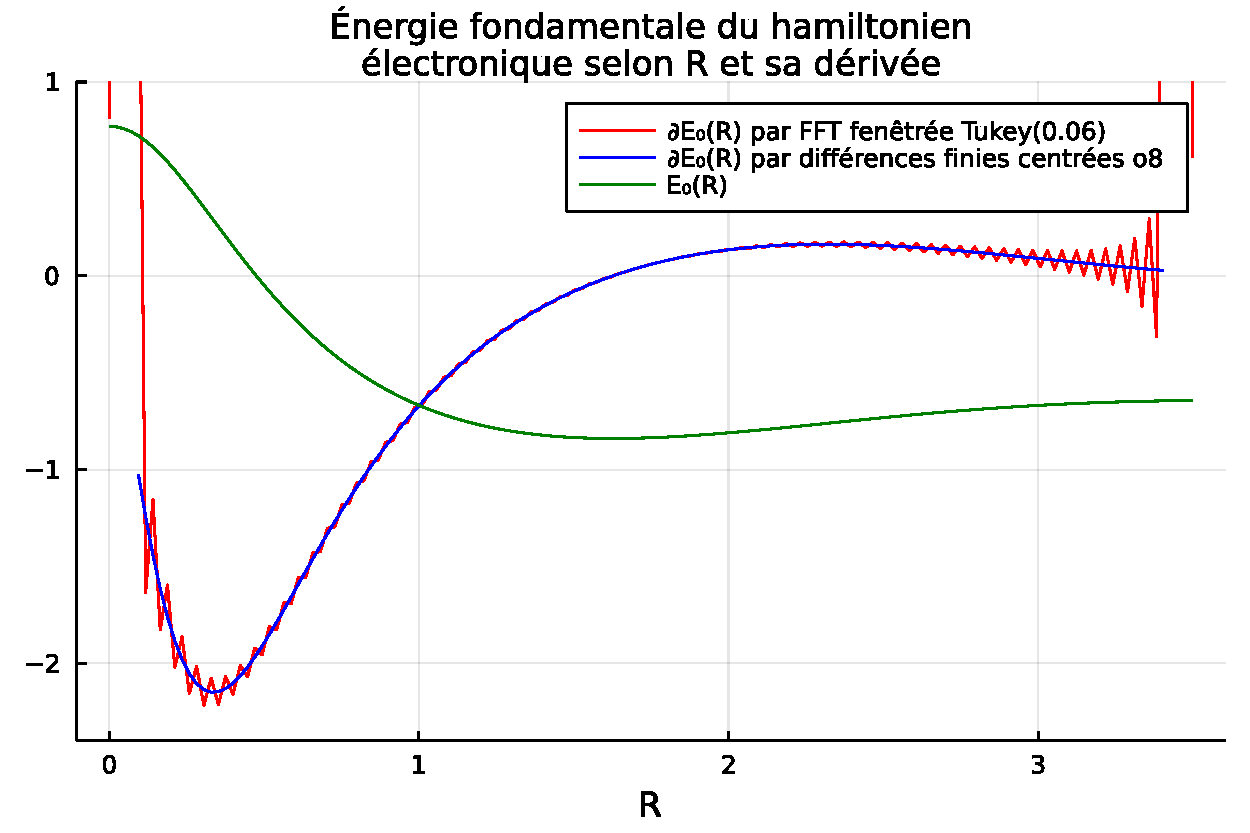
\includegraphics[width=.7\textwidth]{images/énergie_fdmtle_hamiltonien.pdf}
    \caption[Énergie fondamentale $R\mapsto E_0(R)$ et sa dérivée approchée de deux manières différentes.]{Énergie fondamentale $R\mapsto E_0(R)$ et sa dérivée approchée de deux manières différentes en fonction de l'hyperparamètre $R$ (distance entre les 2 nucléons). Chacune a un inconvénient: une dérivée fréquentielle sera difficilement précise en raison des parasites de haute fréquence dûe à la faible longueur du signal, même avec un fenêtrage et les différences finies ont un ordre de précision limité. Les deux nécessitent un échantillonnage qui est totalement bloquant si l'on veut évaluer la dérivée en un point précis hors de l'échantillonnage. Ce ne seront donc pas les approches choisies pour la descente de gradient dans la section \ref{sec:minimum_R}.}
    \label{fig:energie_fdtle_ham}
\end{figure}

\subsection{Obtention de l'argument $R$ minimisant l'énergie de surface}
\label{sec:minimum_R}

\subsubsection{Théorème d'\textsc{Ehrenfest} pour la dérivée}
Pour obtenir l'énergie de surface minimale $E_0$ et le paramètre $R_0$ permettant de l'atteindre, plusieurs méthodes s'offrent à nous. Il s'agit de minimiser une fonction, problème classique en informatique.

Nous allons exploiter une propriété intéressante que j'introduis pour le moment qualitativement: \textbf{lorsque l'on perturbe légèrement un hamiltonien, la modification infinitésimale (à l'ordre 1) sur l'état normé réel (donc le vecteur propre) d'un mode non dégénéré est orthogonale à celui-ci}. Ce résultat est bien connu, la preuve sera reproduite plus loin à la section \ref{title:det_termes_pert}.

Par conséquent, si on se donne un hamiltonien dépendant d'un paramètre $\lambda$ et qu'on se place en un point $\lambda$, avec l'état fondamental $\psi(\lambda)$ et son énergie $E(\lambda)$, la dérivée  l'observable énergie par rapport à  $\lambda$  est:
\begin{equation}
\label{eq:derivee_E_lambda}
    \frac{\mathrm{d}E}{\mathrm{d}\lambda}(\lambda_0) = 2\underbrace{ \left\langle \frac{\mathrm{d}\psi}{\mathrm{d}\lambda}(\lambda_0) | \underbrace{H(\lambda_0) | \psi(\lambda_0)  }_{E(\lambda_0)\psi(\lambda_0)} \right\rangle }_{=0} + \left\langle \psi(\lambda_0) \left| \frac{\mathrm{d}H}{\mathrm{d}\lambda}(\lambda_0) \right| \psi(\lambda_0) \right\rangle
\end{equation}

L'égalité \ref{eq:derivee_E_lambda} est un cas particulier du théorème d'\textsc{Ehrenfest}, qui donne la dérivée d'un observable sans avoir à connaître la dérivée de l'état.


\subsubsection{Choix de l'algorithme d'approche: une méthode de quasi-\textsc{Newton}}

On est donc dans un cas courant, en optimisation, où on connaît la fonction et sa dérivée (exprimée elle-même à l'aide de l'état, voire figure \ref{fig:energie_fdtle_ham}).





Partant de ceci, de nombreuses solutions s'offrent à nous\footnote{Voir également \url{https://ruder.io/optimizing-gradient-descent/index.html}} (liste non exaustive):


\begin{enumerate}
    \item Une dichotomie simple;
    \item Une descente de gradient sur $E(\lambda)$ parmi les nombreuses adaptations existantes selon l'adaptation des pas à chaque étape comme RMSprop, BFGS, ADA-\{Max, M, grad, \dots\} qui apparaissent dans la littérature florissante en Machine Learning notamment;
    \item La méthode de recherche de 0 de \textsc{Newton-Raphson} appliquée à $\frac{\mathrm{d}E}{\mathrm{d}\lambda}$ (nécéssiterait l'accès à $\frac{\mathrm{d}^2E}{\mathrm{d}\lambda^2}$);
    \item Une méthode de recherche de 0 parmi lesdites quasi-\textsc{Newton} (\textsc{Broyden}, \textsc{Davidon-Fletcher-Powell}, etc.), méthode des sécantes, etc., appliquée à $\frac{\mathrm{d}E}{\mathrm{d}\lambda}$ qui s'affranchissent de la connaissance exacte de la jacobienne ou de la hessienne de $\frac{\mathrm{d}E}{\mathrm{d}\lambda}$.
\end{enumerate}

Une solution évidente est la dichotomie pour trouver un zéro de la dérivée de $E(\lambda)$. Cette méthode présente une convergence linéaire (à chaque étape l'erreur est divisée par deux),  c'est-à-dire que l'erreur suit une progression géométrique et on peut atteindre la précision machine en un temps logarithmique (mesuré en nombre d'étapes).

Quitte à devoir évaluer l'état et l'énergie (le plus coûteux) pour obtenir la dérivée (le moins coûteux une fois les précédents acquis) avec \ref{eq:derivee_E_lambda}, autant utiliser la méthode des sécantes qui converge plus rapidement qu'une dichotomie. En voici un pseudo-code élémentaire:

\begin{align*}
\hbox{Inputs }& x_0, x_1, f, \varepsilon \\
\hbox{Processing } & x_{k-1} := x_0 \\
&  x_{k} := x_1 \\
&  x_m := x_1 \\
& \hbox{while } |x_k - x_{k-1}|>\varepsilon  \hbox{ do} \\
& \qquad x_{k} := \frac{x_k-x_{k-1}}{f(x_k)-f(x_{k-1})}f(x_k) \\
& \qquad x_{k-1} := x_m \\
& \hbox{end while} \\
\hbox{Outputs } & x_{k}
\end{align*}

Il s'agit dans l'idée de la métode de \textsc{Newton} avec une approximation de la dérivée de $f$.

\textbf{Compte tenu du caractère un peu particulier de la fonction $R \mapsto E_0(R)$ dont on ne connaît pas de forme algébrique close (mais qui nécessite l'appel à un algorithme d'éléments propres), je n'utiliserai pas les paquets Julia comme \codewordred{Optim} ou \codewordred{Roots}, mais je coderai la méthode des sécantes à la main appliquée à $\frac{\mathrm{d}E}{\mathrm{d}R}$. De même, puisqu'il sera nécessaire d'obtenir une évaluation assez précise de la dérivée de $R\mapsto E(R)$ en tous les points itérés de l'algorithme, il est malaisé d'évaluer ces dérivées par des méthodes de traitement du signal (comme les différences finies ou la dérivation fréquentielle avec \codewordred{FFTW} et \codewordred{DSP} qui a été testée, et qui nécessite d'ailleurs un fenêtrage) car elles se basent sur un échantillonnage. Utiliser ainsi le théorème d'\textsc{Ehrenfest} est par conséquent tout-à-fait justifié et même nécessaire. Voir figure \ref{fig:ehrenfest_erreur}.} 

L'algorithme \ref{alg:calc_en_mini} résume la démarche.

\begin{figure}
    \centering
    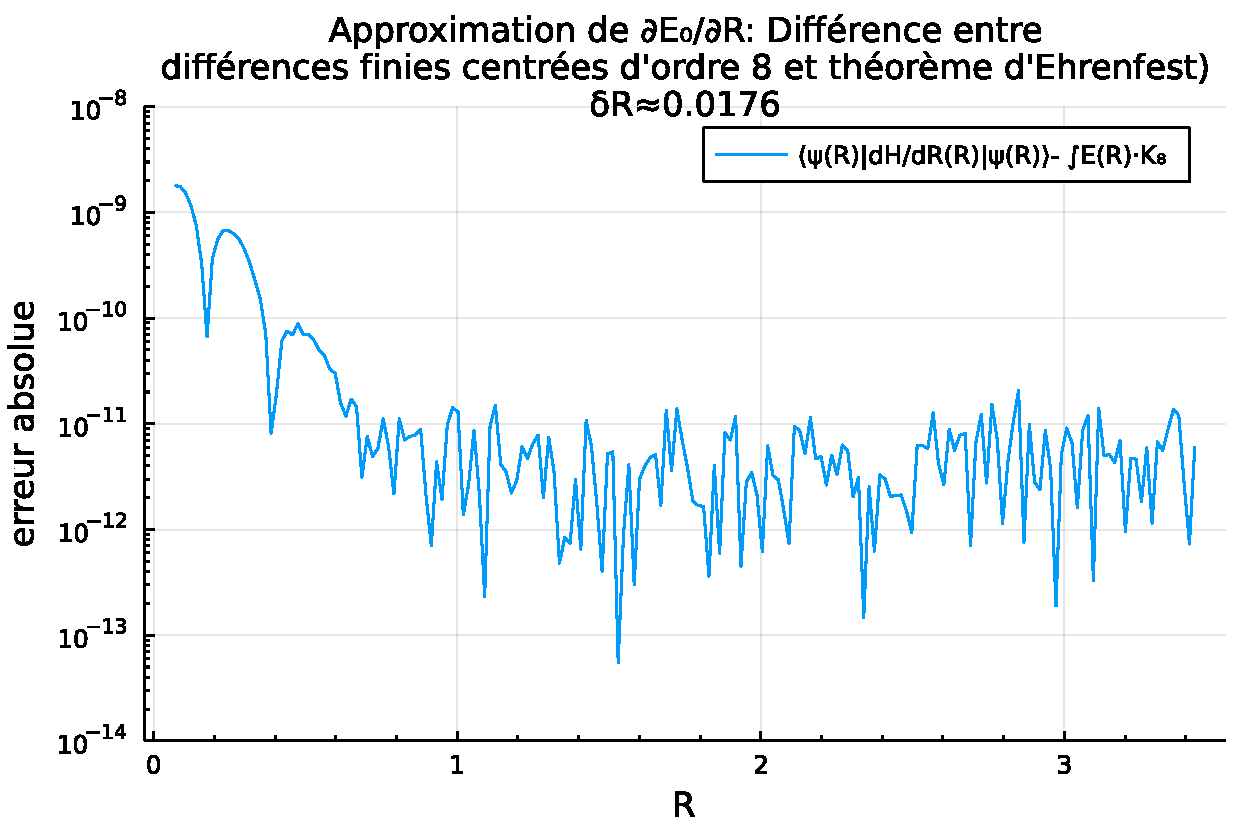
\includegraphics[width=.7\textwidth]{images/erreur_dérivée.pdf}
    \caption[Différence entre la dérivée de $E_0(R)$ calculée en différences finies centrées d'ordre 8 et avec le théorème d'\textsc{Ehrenfest}.]{Différence entre la dérivée de $E_0(R)$ calculée en différences finies centrées d'ordre 8 et avec le théorème d'\textsc{Ehrenfest}.}
    \label{fig:ehrenfest_erreur}
\end{figure}



\begin{algorithm}[H]
\caption{Calcul du paramètre nucléaire minimisant l'énergie fondamentale}
\label{alg:calc_en_mini}
\begin{algorithmic}[1]
\Require $\Lambda_r: \in \mathscr{M}_{n,n}(\mathbb{R}); R_g \in \mathbb{R}$ (laplacien suivant l'axe des $r$); $R^\dagger, R^\ddagger \in \mathbb{R}$ (points de départ); $\varepsilon>0$ (précision); $\mathcal{V} : \mathbb{R} \rightarrow \mathbb{R}$ (fonction potentiel d'interaction noyau-électron); $\mathcal{V}^\prime$ (sa dérivée); $\mathbf{r}_s$ (vecteur ordonné des $r$ sur la grille)
\Ensure $R_0 = \argmin_{R\in\mathbb{R}} E_0(R)$ à $\varepsilon$ près
\Procedure{Méthode des sécantes appliquée à $\frac{\mathrm{d}E}{\mathrm{d}R}$}{}
\State $\partial E^\ddagger \gets \varepsilon +1$



\While{$|\partial E^\ddagger| > \varepsilon$}
\State $\hat{H}^\dagger \gets \Lambda_r + \text{diag}\left( \mathcal{V}(\mathbf{r}_s+\frac{R^\dagger}{2}) + \mathcal{V}(\mathbf{r}_s-\frac{R^\dagger}{2})\right)$

\State $\hat{H}^\ddagger \gets \Lambda_r + \text{diag}\left( \mathcal{V}(\mathbf{r}_s+\frac{R^\ddagger}{2}) + \mathcal{V}(\mathbf{r}_s-\frac{R^\ddagger}{2})\right)$

\State $\psi^\dagger \gets \argmin \text{Sp}( \hat{H}^\dagger)$ \Comment{Avec \codewordred{KrylovKit}}

\State $\psi^\ddagger \gets  \argmin \text{Sp}(\hat{H}^\ddagger)$ 
\State $\partial\hat{H}^\dagger \gets \text{diag}\left( \frac{1}{2} \mathcal{V}^\prime(\mathbf{r}_s+\frac{R^\dagger}{2}) - \frac{1}{2} \mathcal{V}^\prime(\mathbf{r}_s-\frac{R^\dagger}{2})\right)$
\State $\partial\hat{H}^\ddagger \gets  \text{diag}\left( \frac{1}{2} \mathcal{V}^\prime(\mathbf{r}_s+\frac{R^\ddagger}{2}) - \frac{1}{2} \mathcal{V}^\prime(\mathbf{r}_s-\frac{R^\ddagger}{2})\right)$
\State $\partial E^\dagger \gets \langle \psi^\dagger | \partial\hat{H}^\dagger | \psi^\dagger \rangle$ \Comment{Optimisé  avec \codewordgreen{dot}}
\State $\partial E^\ddagger \gets \langle \psi^\ddagger | \partial\hat{H}^\ddagger | \psi^\ddagger \rangle$
\State $(R^\ddagger, R^\dagger) \gets \left( R^\ddagger - \frac{ R^\ddagger- R^\dagger}{\partial E^\ddagger-\partial E^\dagger} \partial E^\ddagger, R^\ddagger\right)$ \Comment{Descente du gradient de $\frac{\mathrm{d}E}{\mathrm{d}R}$}
\EndWhile
\EndProcedure
\Return $R^\ddagger$
\end{algorithmic}
\end{algorithm}

\begin{remark}
En pratique, on peut baisser la complexité mémoire de l'algorithme \ref{alg:calc_en_mini} en panachant les calculs de chaque hamiltonien et de sa dérivée à stocker dans une même variable avant son utilisation. C'est ce que j'ai fait en pratique mais pour la compréhension visuelle, j'ai laissé l'algorithme tel quel ici. Ci-après, le code Julia correspondant avec ces optimisations pour mémoire.
\end{remark}



\begin{codejulia}{Code Julia de l'algorithme \ref{alg:calc_en_mini}}
Hr = copy(Λr); # initialisation opérateurs
dHr = Diagonal(zeros(N)); 
iter_nb = 0;
dE_rp = |$\epsilon$| +1; # initialisation pour rentrer dans la boucle

while (iter_nb < itermax && abs(dE_rp) > |$\epsilon$|)
    # calcul des états
    Hr[diagind(Hr)] = diag(Λr) + Vector(V_nucl_el.(rs, R_rp)) .+ V_nucl_nucl(R_rp);
    vals, vecs, infos = KrylovKit.eigsolve(Hr, N, 1, :SR, krylovdim=kdim1d, issymmetric=true, ishermitian=true);
    @assert infos.converged > 0;
    |$\psi$|_rp = Vector(vecs[1]);

    Hr[diagind(Hr)] = diag(Λr) + Vector(V_nucl_el.(rs, R_lp)) .+ V_nucl_nucl(R_rp);
    vals, vecs, infos = KrylovKit.eigsolve(Hr, N, 1, :SR, krylovdim=kdim1d, issymmetric=true, ishermitian=true);
    @assert infos.converged > 0;
    |$\psi$|_lp = Vector(vecs[1]);

    # calcul des dérivées de l'énergie
    dHr[diagind(dHr)] = dR_V_nucl_el.(rs, R_rp) .+ dV_nucl_nucl(R_rp); 
    dE_rp = dot(|$\psi$|_rp,dHr,|$\psi$|_rp); 
    

    dHr[diagind(dHr)] = dR_V_nucl_el.(rs, R_lp) .+ dV_nucl_nucl(R_lp);
    dE_lp = dot(|$\psi$|_lp,dHr,|$\psi$|_lp);

    # méthode des sécantes pour la dérivée de l'énergie par rapport à R
    R_rp_mem = R_rp;
    step = dE_rp*(R_rp-R_lp)/(dE_rp-dE_lp);
    R_rp -= step;
    R_lp = R_rp_mem;
    iter_nb += 1;

    @show iter_nb, step, dE_rp;
end
\end{codejulia}



\subsection{Scission du potentiel en un hamiltonien non perturbé et une perturbation}
\label{sec:scission_potentiel}
\textbf{Dorénavant j'effectue le remplacement\footnote{Pour éviter toute ambiguïté liée à des erreurs de typographie} de noms des variables $r \rightsquigarrow x$ et $R \rightsquigarrow y$ (et $R_0=y_0$).}

\textbf{Le point charnière de ce stage se résume dans la décomposition suivante (proposée par le tuteur scientifique):}


\begin{multline}
    \hat{H} = \textcolor{RawSienna}{E_0(y_0)} 
     - \frac{1}{2M} \frac{\partial^2}{\partial y^2} \textcolor{PineGreen}{+ \frac{1}{2} \frac{\mathrm{d}^2 E_0}{\mathrm{d}y^2}(y_0)(y-y_0)^2} \\
     - \frac{1}{2m} \frac{\partial^2}{\partial x^2} \textcolor{NavyBlue}{+ V(x,y_0)}   \textcolor{RawSienna}{- E_0(y_0)} \\
     + V(x,y) \textcolor{NavyBlue}{- V(x,y_0)} \textcolor{PineGreen}{- \frac{1}{2} \frac{\mathrm{d}^2 E_0}{\mathrm{d}y^2}(y_0)(y-y_0)^2}
\end{multline}

Le hamiltonien de départ $\hat{H}$ se décompose donc sous la forme de deux hamiltoniens non perturbés $\hat{H}^0_y$ et $\hat{H}^0_x$ agissant chacun respectivement sur une coordonnée généralisée (chacune sur la même variable d'espace, selon un axe unidimensionnel), et un terme de couplage entre ces deux coordonnées $\hat{W}$, que l'on traitera comme une perturbation:

\begin{equation}
    \hat{H} = \hat{H}^0_y + \hat{H}^0_x + \hat{W} 
\end{equation}

\begin{equation}
\label{3termes}
       \left\{  \begin{array}{ll}
        \hat{H}^0_y &= 
     - \frac{1}{2M} \frac{\partial^2}{\partial y^2} + \frac{1}{2} \frac{\mathrm{d}^2 E_0}{\mathrm{d}y^2}(y_0)(y-y_0)^2 +E_0(y_0) \\
        \hat{H}^0_x &= - \frac{1}{2m} \frac{\partial^2}{\partial x^2} + V(x,y_0) -E_0(y_0) \\
        \hat{W}_2 &=   V(x,y) - V(x,y_0) - \frac{1}{2} \frac{\mathrm{d}^2 E_0}{\mathrm{d}y^2}(y_0)(y-y_0)^2
    \end{array}\right.
\end{equation}


Ensuite, on se place en $(x,y_0)$ pour écrire le développement limité de $V$ dans le terme $W$:
\begin{equation}
    V(x,y) - V(x,y_0) = \frac{\partial V}{\partial y}(x,y_0)(y-y_0) + \frac{1}{2}\frac{\partial^2V}{\partial y^2}(x,y_0)(y-y_0)^2 + \underset{y\rightarrow y_0}{o} (y-y_0)^2 
\end{equation}

Finalement,
\begin{equation}
    \boxed{\hat{W} = \frac{\partial V}{\partial y}(x,y_0)(y-y_0)  + \frac{1}{2} \left(\frac{\partial^2V}{\partial y^2}(x,y_0) -\frac{\mathrm{d}^2 E_0}{\mathrm{d}y^2}(y_0) \right)   (y-y_0)^2 + \text{h.o.t.}}
\end{equation}






\section{Changement de variable et adimensionnement}
\label{sec:chgt_var_adim}
On peut alors traiter ce problème en essayant de trouver de manière approchée, une solution au problème simplifié $\hat{H} -  \text{h.o.t.} = \hat{H}^0_y + \hat{H}^0_x + \hat{W} -  \text{h.o.t.}$  pour lequel on néglige les termes d'ordre supérieurs ou égal à 3. Cela revient donc à prendre  en lieu et place de $\hat{W}$, la perturbation tronquée $\tilde{\hat{W}}$ de ces termes suivante:
\begin{equation}
\label{W_pert_tronque}
    \tilde{\hat{W}} = \frac{\partial V}{\partial y}(x,y_0)(y-y_0)  + \frac{1}{2} \left(\frac{\partial^2V}{\partial y^2}(x,y_0) -\frac{\mathrm{d}^2 E_0}{\mathrm{d}y^2}(y_0) \right)   (y-y_0)^2 
\end{equation}

On remarque d'ailleurs que la perturbation $W$ est elle-même une somme de termes séparable en les variables $x$ et $y$.

À partir de là, on traite le terme $\hat{H}^0_x$ du hamiltonien non perturbé analytiquement puisqu'il s'agit d'un oscilateur harmonique, le terme $\hat{H}^0_y$ numériquement, à partir desquels on construit une solution $\Psi^{\text{HBO}} (x,y) = \psi^0_{y_0}(x) \phi^0(y)$ (HBO signifie \textit{Harmonic Born-Oppenheimer}.) Puis, on applique la théorie des perturbations à $\Psi^{\text{HBO}}$ et $\tilde{\hat{W}}$. 

Nous aurons donc deux leviers d'action sur le développement: l'ordre du DSE en espace, et l'ordre de la perturbation.


\paragraph{Erreur commise}
Dans cette démarche on commet des erreurs dans l'approximation de l'état fondamental à trois niveaux:
\begin{enumerate}
    \item En discrétisant l'espace de dimension infinie dans lequel existe la fonction d'onde, et en l'approchant par un \og représentant \fg{}\footnote{Abus de langage mathématique.} dans un espace de dimension finie (qui ne recouvre pas tout l'espace), ainsi que ses dérivées (approchées par différences finies);
    \item Lors de l'approximation de la perturbation $\hat{W}$ par $\tilde{\hat{W}}$ avec son développement limité;
    \item Lors de l'approximation de la fonction d'onde en tronquant le développement de la perturbation à un ordre fini.
\end{enumerate}



\subsubsection{Adimensionnement du problème suivant la dimension nucléaire}
Le but étant d'étudier la validité de \textsc{Born-Oppenheimer} lorsque la masse des protons devient grande devant celle de l'électron, on verra la fonction d'onde s'écraser suivant une dimension, car les protons deviennent peu à peu classiques. Pour ne pas impacter la simulation numérique, on va adimensionner le problème suivant la variable $R$.

Dans l'équation \ref{3termes}, on a vu que le hamiltonien suivant l'axe $(Oy)$ (rappelons-le, $y \equiv R$), il s'agit d'un oscillateur. Comme vu dans le théorème \ref{bo_osc_harm}, la solution fondamentale de l'oscillateur est une gaussienne de longueur caractéristique $\sqrt{\frac{2\hbar}{M\omega^2}}$ (cf. équation \ref{formule_osc_gauss_bis}).

Pour adimensionner avec notre cas, à savoir la constante de raideur $K =M\omega^2=\frac{\mathrm{d}^2 E_0}{\mathrm{d}y^2}(y_0)$,  il est donc naturel\footnote{C'est aussi ce que l'on trouve avec l'approximation BKW (\ref{bkw_approx}).} de poser $y \equiv R = R_0 + \varepsilon u$ avec $\varepsilon = (MK)^{-1/4}$, on a ainsi centré le problème autour de la distance nucléaire d'équilibre.

Les hamiltoniens \ref{3termes} reparamétrés deviennent



%\# FAIRE LA DEMONSTRATION \#
\begin{equation}
\label{3termes_bis}
       \left\{  \begin{array}{ll}
        \mathfrak{h}_u &= K\varepsilon^2  \left( -\frac{1}{2} \frac{\partial^2}{\partial u^2} + \frac{1}{2}u^2\right)  + E_0(R_0) \\
        \mathfrak{h}_x &= - \frac{1}{2m} \frac{\partial^2}{\partial x^2} + V(x,R_0) -E_0(R_0) \qquad \qquad \text{(inchangé: $\mathfrak{h}_x=\hat{H}^0_x$)}\\
        \mathfrak{w} &=   V(x,R_0 + \varepsilon u) - V(x,R_0) - \frac{\varepsilon^2 K}{2} u^2    \end{array}\right.
\end{equation}

puis le DSE en espace de la perturbation ici à l'ordre 2:

\begin{equation}
\label{W_pert_tronque_bis}
     \hat{\mathfrak{w}} = \varepsilon \frac{\partial V}{\partial y}(x,y_0)u  + \frac{1}{2} \varepsilon^2 \left(\frac{\partial^2V}{\partial y^2}(x,y_0) -K \right)   u^2
\end{equation}


\textbf{Par conséquent on a mis au point deux  paramètres déterminants pour notre approximation: $\varepsilon$ et l'ordre du DL pour $\frak{w}$, sur lesquels on peut jouer.}






\section{Théorie des perturbations à tout ordre sur le système d'intérêt}

\subsection{Théorie des perturbations: présentation}

Je présente ici une méthode d'approximation d'états propres en physique qui très connue et présente en particulier dans beaucoup d'ouvrages de mécanique quantique. Elle n'est pas exclusive à ce domaine, et repose sur des théorèmes mathématiques qui sont présentés ultérieurement. Elle trouve naturellement beaucoup d'applications en physique de manière générale. Les résultats qui suivent ne sont ainsi pas inédits: je reprends l'état de l'art en redémontrant certains points plus précisément que certains ouvrages. 


Supposons que l'on dispose d'un hamiltonien $\hat{H} = \hat{H}^0 +  \lambda \hat{W}$ dont les solutions stationnaires pour $\hat{H}^0$ sont connues et discrètes, notées $(\mathcal{E}_k,|\phi_k \rangle)_{k\in\mathbb{N}}$, et formant une base de l'espace hilbertien auquel ils appartiennent. La théorie des perturbations suppose que l'on peut approcher la solution de $\hat{H}$ à partir de celles de $\hat{H}^0$. Plus précisément, on fait l'hypothèse que le $j$-ième mode perturbé $(E(\lambda),|\psi(\lambda) \rangle)$ de $\hat{H}$ avec $|\psi(\lambda)\rangle$ \textbf{normé},  s'obtient par un développement en séries de \textsc{Taylor}:

\begin{equation}
    E(\lambda) =  \sum_{k=0}^{+\infty} \lambda^k E_k \qquad |\Psi(\lambda)\rangle = \sum_{k=0}^{+\infty} \lambda^k |\psi_k\rangle
\end{equation}
où les $(E_k,|\psi_k\rangle)$ sont à déterminer. En général, dans la littérature, on se contente de l'ordre 1 ou 2, surtout pour un espace hilbertien de dimension infinie, et cela donne lieu à ce qu'on appelle une \textit{contamination} de l'état non perturbé considéré par les autres non perturbés après ajout de la perturbation.




Le fait que les états (resp. les  énergies) soient développables en série entière autour de l'état non perturbée (resp. l'énergie non perturbée) n'est pas évident. En dimension finie, cela impose la différentiabilité de $\hat{H} \mapsto (E_j,|\psi_j \rangle)$ dans la direction $\hat{W}$ en $\hat{H}^0$ à tout ordre, mais \cite{cohen-tannoudji_mecanique_2021-1} admet cela comme une hypothèse commode. 

Notons que pour que ces calculs soient exacts, il est nécessaire que la valeur propre $E_j$ considérée ne soit pas dégénérée (de multiplicité au plus 1). Ce n'est pas très gênant pour les cas qui nous intéressent dans le cadre de ce stage, puisque nous l'appliquerons surtout à la plus petite valeur propre d'un système pour connaître son état fondamental, non dégénéré pour le hamiltonien qui nous intéresse.


En fait, cette hypothèse de développement en série entière est justifiée, au moins en dimension finie pour l'énergie dans \cite{reed_methods_1980}, le théorème XII.1 stipule que:
\begin{theorem}{(\cite{reed_methods_1980},  théorème XII.1)}
    Si $F(\beta,\gamma) = \gamma^n + a_1(\beta)\gamma^{n-1}+\cdots + a_n(\beta)$ est un polynôme de degré $n$ dont les coefficients sont analytiques en $\beta$ (i.e., développables en série entière sur une boule de rayon non nul autour de tout point de  $\mathbb{C}$), et soit $\gamma_0$ une racine simple de $\gamma \mapsto F(\beta_0,\gamma)$ pour un certain $\beta_0$, alors pour $\beta$ suffisamment proche de $\beta_0$, il existe une unique racine $\gamma(\beta)$ de la fonction $\gamma \mapsto F(\beta,\gamma)$ proche de $\gamma_0$ et $\beta \mapsto \gamma(\beta)$ est analytique en $\beta$ autour de $\beta_0$.
\end{theorem}


Si on applique ce théorème au polynôme caractéristique $\det (\gamma I_n -( H_0 + \beta W))$ qui est de coefficient de terme de plus haut degré égal à 1 (en $\gamma$), on obtient que l'énergie propre obtenue suite à une perturbation \og petite \fg{} du hamiltonien, est bien dévelopable en séries entière autour de l'énergie propre non-dégénérée correspondante au hamintonien non perturbé et le DSE de l'énergie dont les coefficients sont appelés coefficients  de \textsc{Rayleigh-Schrödinger}. Ce même livre donne aussi un théorème justifiant l'existence du DSE pour le vecteur propre correspondant (théorème II.4, \cite{reed_methods_1980}), que j'élude ici.

Remarquons que plus simplement, si on l'applique à $\det (\gamma I_n -H(\beta))$ avec $H$ analytique en $\beta$, on obtient la condition de régularité nécessaire pour l'algorithme des sécantes fait à la section précédente, puisque la fonction de potentiel choisie dans \ref{potentiel_H2plus} est analytique en $R$. Ainsi $R \mapsto E_0(R)$ est au moins de classe $\mathscr{C}^2$ ce qui permet d'appliquer la méthode des sécantes.

\subsubsection{Identification à chaque ordre des termes de la série}
Pour déterminer les $(E_k,|\psi_k\rangle)$, on écrit les égalités des termes de même ordre dans l'équation d'une perturbation en $\lambda$:
\begin{equation}
    (\hat{H}^0 + \lambda \hat{W}) \left(  \sum_{k=0}^{+\infty} \lambda^k |\psi_k\rangle \right) = \left(  \sum_{k=0}^{+\infty} \lambda^k E_k \right) \left( \sum_{k=0}^{+\infty} \lambda^k |\psi_k\rangle \right)
\end{equation}




Pour déterminer successivement les énergies propres et vecteurs propres de ce développement, on commence par identifier les termes d'ordre 1, puis 2, puis 3, etc., ce qui est licite, au moins en dimension finie, en raison de l'unicité des coefficients d'une série entière. Cela donne successivement comme dans \cite{cohen-tannoudji_mecanique_2021-1}:
\begin{align}
    (\hat{H}^0-E_0) |\psi_0\rangle &= 0 \, \text{(ordre 0)}\label{ordre0} \\
    (\hat{H}^0-E_0) |\psi_1\rangle + (\hat{W}-E_1) |\psi_0\rangle &=0 \, \text{(ordre 1)} \label{ordre1} \\
    (\hat{H}^0-E_0) |\psi_2\rangle + (\hat{W}-E_1) |\psi_1\rangle - E_2 |\psi_0\rangle &= 0 \, \text{(ordre 2)}  \label{ordre2}\\
    &\vdots \\
    (\hat{H}^0 - E_0) |\psi_q\rangle + (\hat{W}-E_1)|\psi_{q-1}\rangle -E_2 |\psi_{q-2}\rangle + \dots - E_q |\psi_0\rangle &= 0 \, \text{(ordre $q$)} \label{ordreq}
\end{align}

Si l'on cherche à estimer un état non dégénéré $(\mathcal{E}_j, |\phi_j\rangle)$ après perturbation en le choisissant réel (phase nulle) et normé, on montre ainsi, en faisant $\lambda \rightarrow 0$, que $E_0 = \mathcal{E}_j$ et $|\psi_0 \rangle = |\phi_j\rangle$ ce qui permet d'écrire plus précisément
\begin{equation}
    (\hat{H}^0 + \lambda \hat{W}) \left( |\phi_j\rangle + \sum_{k=1}^{+\infty} \lambda^k |\psi_k\rangle \right) = \left( \mathcal{E}_j + \sum_{k=1}^{+\infty} \lambda^k E_k \right) \left(|\phi_j\rangle + \sum_{k=1}^{+\infty} \lambda^k |\psi_k\rangle \right)
\end{equation}

c'est-à-dire que l'on a déjà déterminés $|\psi_0\rangle$ et $E_0$. Il ne reste plus qu'à trouver les autres. 



\subsection{Détermination des termes grâce à la méthode de la \textit{sum over states}}
\label{title:det_termes_pert}

On va montrer que cette méthode est peu adaptée en prenant l'exemple de l'oscillateur harmonique quantique 2D.

À partir d'ici, je vais décrire et prouver un algorithme à l'aide des formules systématiques à tout ordre, comme dans \cite{cohen-tannoudji_mecanique_2021-1} pour déterminer les états et énergies des développements de \textsc{Taylor}. Ce n'est donc pas un travail inédit, mais je m'efforce de justifier un peu mieux les égalités que ce que j'ai pu lire dans la littérature.





\subsubsection{Détermination des termes de l'état propre}

Pour exprimer les états $|\psi_k\rangle$, on va les décomposer dans la base orthonormale des états propres du hamiltonien non perturbé $|\phi_k\rangle$, les vecteurs $|\phi_j \rangle$, ce qui est toujours faisable car on a supposé être en dimension finie et s'être muni d'une base de vecteurs propres de cet espace. 

Notons donc  pour tout ordre $q$,   
\begin{equation}
    |\psi_q \rangle = \sum_k \alpha_k^{(q)} |\phi_k \rangle; \quad \alpha_k^{(q)} = \langle \psi_q | \phi_k \rangle
\end{equation}

On détermine ensuite les $(\alpha^{(q)}_k), 1\le k \le \dim \mathscr{H}, q\in\mathbb{N}$ par récurrence sur $q$. L'hypothèse de choix $|\psi(\lambda)\rangle$ \textbf{réel normé} est fondamentale car elle permet dans les calculs suivants de rendre la symétrie au produit scalaire de deux états et d'écrire pour tout $q$ en développant $1 = \left\| \mathcal{O}(\lambda^{q+1}) +  \sum_{i=0}^q \lambda^i \psi_i  \right\|^2$, que:
\begin{equation}
    \sum_{s=1}^q \lambda^s \sum_{i=0}^s \langle \psi_i | \psi_{s-i} \rangle + \mathcal{O} ( \lambda^{q+1}) = 0
\end{equation}
et on impose donc
\begin{equation}
\label{astuce_calc}
    \sum_{s=1}^q \lambda^s \sum_{i=0}^s \langle \psi_i | \psi_{s-i} \rangle = 0
\end{equation}

\begin{itemize}
    \item Dans un premier temps, Pour déterminer $\alpha_j^{(q)}$ (rappelons que $j$ est l'indice du mode que l'on essaie d'estimer après perturbation), on a recours à l'astuce suivante comme on trouve dans la littérature, dont je rédige la preuve plus précisément et à tout ordre:


\begin{figure}[H]
    \centering
    \includegraphics[scale=1.3]{images/explication_développement.pdf}
    \caption{Développement des termes de $\langle \psi(\lambda )| \psi(\lambda ) \rangle$ à l'ordre $q$.}
    \label{fig:explications_dvp}
\end{figure}


\begin{itemize}
    \item Pour l'ordre 1, en écrivant $1= \langle \psi(\lambda )| \psi(\lambda ) \rangle = \langle \psi_0| \psi_0 \rangle + \lambda \langle \psi_1 | \psi_0 \rangle + \lambda \langle \psi_0 | \psi_1 \rangle + \mathcal{O}(\lambda^2) = 1$ sachant que $|\psi_0\rangle = |\phi_j\rangle$ et que tous les états non perturbés sont normés et réels, et que les $|\psi\rangle$ sont également choisis réels,  en faisant tendre $\lambda$ vers 0, on déduit par croissance comparée que $2\Re (\langle \psi_0 | \psi_1 \rangle) = 2 \langle \psi_1 | \psi_0 \rangle = 0$ autrement dit, $| \psi_1 \rangle$ est orthogonal à $| \psi_0 \rangle$, il n'y a pas de composante sur $|\phi_j\rangle$ à l'ordre 1, soit encore 
    \begin{equation}
        \boxed{\alpha_j^{(1)} =  0}
    \end{equation}
    \item Pour l'ordre $q \ge 2$, en suivant le groupement des termes présenté dans la figure \ref{fig:explications_dvp}: 
    \begin{multline}
    \label{calcul_alphaj}
        1 = \langle \psi(\lambda )| \psi(\lambda ) \rangle = \left\| \mathcal{O}(\lambda^{q+1}) +  \sum_{i=0}^q \lambda^i \psi_i  \right\|^2 = \mathcal{O}(\lambda^{q+1}) + 2 \lambda^q \langle \psi_0 | \psi_q\rangle + \lambda^q \sum_{i=1}^{q-1} \langle \psi_i |\psi_{q-i} \rangle \\
        + \underbrace{\langle \psi_0 | \psi_0 \rangle}_{=1} + \sum_{s=1}^{q-1} \sum_{\substack{u,v \ge 0 \\ u+v=s}} \lambda^s \langle \psi_u | \psi_v \rangle 
    \end{multline}
    On peut alors utiliser  \ref{astuce_calc} dans le dernier terme de \ref{calcul_alphaj} et on obtient donc après soustraction de 1 des deux côtés et réarrangement:
    \begin{equation}
        2 \lambda^q \langle \psi_0 | \psi_q\rangle = - \lambda^q \sum_{i=1}^{q-1} \langle \psi_i |\psi_{q-i} \rangle + \mathcal{O}(\lambda^{q+1})
    \end{equation}
    Il ne reste plus qu'à diviser cette égalité par $\lambda^q$, puis en faisant $\lambda \rightarrow 0$ on obtient:
    \begin{equation}
    \label{phijpsiq}
        \boxed{\alpha^{(q)}_j = \langle \phi_j | \psi_q\rangle=-\frac{1}{2}\sum_{i=1}^{q-1} \langle \psi_i |\psi_{q-i} \rangle }
    \end{equation}
    et on remarque que la formule reste en fait valable pour $q=1$ (somme vide donne résultat nul).
\end{itemize}




 \item Dans un second temps on détermine les $\alpha_k^{(q)}$ avec $k \neq j$:
 \begin{itemize}
     \item Pour déterminer $\alpha_k^{(1)}$  on reprend \ref{ordre1}:
     \begin{equation}
        \langle \phi_k|\hat{H}^0 - E_0 |\psi_1\rangle + \langle \phi_k | \hat{W}-E_1|\psi_{0}\rangle = 0
     \end{equation}
     ce qui permet d'extraire,  en se souvenant que $E_0 = \mathcal{E}_j$ et que les $\phi_k$ sont vecteurs propres de $\hat{H}^0$, et que $\langle \psi_k | \psi_0\rangle = \langle \psi_k | \phi_j\rangle = 0$ avec $k\neq j$:
     \begin{equation}
         (\mathcal{E}_k-\mathcal{E}_j) \langle \phi_k | \psi_1 \rangle + \langle \phi_k | \hat{W} | \phi_j \rangle = 0
     \end{equation}
     \begin{equation}
         \boxed{\alpha^{(1)}_k = \frac{-\langle \phi_k | \hat{W} | \phi_j\rangle}{\mathcal{E}_k-\mathcal{E}_j} = \frac{-\langle \phi_k | \hat{W} | \psi_0\rangle}{\mathcal{E}_k-\mathcal{E}_j}}
     \end{equation}
     

  \item Puis, pour déterminer n'importe quel $\alpha_k^{(q)}$ on reprend \ref{ordreq} auquel on applique $\langle \phi_k|$:
\begin{equation}
    \langle \phi_k|\hat{H}^0 - E_0 |\psi_q\rangle + \langle \phi_k | \hat{W}-E_1|\psi_{q-1}\rangle - \sum_{i=2}^{q} E_i \langle \phi_i | \psi_{q-i}\rangle  = 0
\end{equation}
d'où, avec les mêmes arguments:
\begin{equation}
\label{alphaknjq}
\boxed{
    \alpha_k^{(q)} = \langle \phi_k | \psi_q\rangle = \frac{1}{\mathcal{E}_k-\mathcal{E}_j} \left[ - \langle \phi_k | \hat{W}-E_1|\psi_{q-1} \rangle + \sum_{i=2}^q E_i \langle \phi_i |\psi_{q-i} \rangle \right]}
\end{equation}
 \end{itemize}
\end{itemize}


\subsubsection{Détermination des termes d'énergie propre}
Pour trouver les énergies $E_k$, on projette chaque équation du hamiltonien d'ordre $k$ sur le vecteur $|\phi_j\rangle$.
\begin{itemize}
    \item En appliquant $\langle \phi_j| $ à \ref{ordre1} (ordre 1) on obtient
    \begin{equation}
        \langle \phi_j| \hat{H}^0-E_0| \psi_1\rangle + \langle \phi_j | \hat{W}-E_1|\psi_0 \rangle = 0
    \end{equation}
    donc puisque $\langle\psi_1 | \phi_j\rangle = 0$ et que les $|\phi_i\rangle$ sont des vecteurs propres pour $\hat{H}^0$, le premier terme du membre de gauche est nul donc cela donne
    \begin{equation}
        \label{en_E1}
        \boxed{E_1 = \langle \phi_j | \hat{W} | \phi_j \rangle}
    \end{equation}
    \item En appliquant $\langle \phi_j| $ à \ref{ordreq} (ordre $q\ge 2$) on obtient, toujours avec $E_0=\mathcal{E}_j$:\footnote{Avec la même convention de somme nulle si son ensemble d'indices est vide.}
    \begin{equation}
        \langle \phi_j| \hat{H}^0-\mathcal{E}_j| \psi_q \rangle + \langle \phi_j | \hat{W}-E_1|\psi_{q-1} \rangle  - \sum_{i=2}^q E_i \langle \phi_j | \psi_{q-i} \rangle = 0
    \end{equation}
    puis comme $\hat{H}^0$ est auto-adjoint, $\langle \phi_j| \hat{H}^0-\mathcal{E}_j| \psi_q \rangle = \langle \psi_q | \hat{H}^0-\mathcal{E}_j|\phi_j  \rangle = 0$, on peut extraire $E_q$:
    \begin{equation}
    \label{enqnj}
        \boxed{E_q =  \langle \phi_j | \hat{W}-E_1 | \psi_{q-1}\rangle - \sum_{i=2}^{q-1} E_i \langle \phi_j | \psi_{q-i}\rangle}
    \end{equation}
\end{itemize}

\subsubsection{Synthèse du calcul}
On peut résumer les calculs à effectuer et leurs dépendances à chaque étape dans le diagramme \ref{fig:causalité}. Ces  6 formules encadrées (ordre 1 + ordre $q\ge 2$) $\times$ (1 terme d'énergie + 2 termes de composantes vecteurs) formules sont très facilement automatisables en informatique et permettent ainsi  de calculer à tout ordre la méthode des perturbations pour l'état propre. Mais dans le code, il faut faire attention à calculer le terme d'énergie avant les composantes, qui l'utilisent majoritairement.

\begin{figure}[H]
    \centering
    \includegraphics[scale=1]{images/causalité_calcul.pdf}
    \caption[Causalité dans le calcul des termes des développements pour la \textit{sum over states}]{Relations de causalité dans le calcul des termes des développements respectifs de l'énergie et de l'état propre après perturbation à tout ordre $q\ge 2$. En pratique il faudra donc calculer l'énergie à l'ordre $q$ avant les coefficients du mode d'ordre $q$ dans la base de décomposition.}
    \label{fig:causalité}
\end{figure}



\subsubsection{Complexité asymptotique}
En notant $N=n\times n$ la dimension de l'espace de \textsc{Hilbert} dans lequel nos états sont calculés (le nombre de points sur la grille), à l'étape $q \ge 2$, sachant les élements des étapes $\le q-1$, le coût des étapes déterminantes en multiplications ou divisions pour obtenir le vecteur $\psi_j$ et le terme d'énergie $E_q$ est 

\begin{multline}
    c_q = \underbrace{1+(q-1) \times \mathrm{N} }_{\alpha_j^{(q) }(\ref{phijpsiq})} + \underbrace{N\times N^2 + (q-1)\times (1+ N)}_{\alpha_{k\neq j}^{(q)} (\ref{alphaknjq})} + \underbrace{N\times N^2+(q-3) \times N}_{E_q (\ref{enqnj})} \\
    = 2N^3 + 3qN - 5N + 2q - 3
\end{multline}

et le coût total de calcul de l'étape 2 à l'étape $Q_\text{max}$ est donc
\begin{equation}
    \sum_{q=2}^{Q_\text{max}} c_q = -2N^3 + \frac{1}{2}(3N + 2)Q_\text{max}^2 + \frac{1}{2}(4N^3 - 7N - 4)Q_\text{max} + 2N + 1 = \boxed{\mathcal{O}(NQ_\text{max}^2) + \mathcal{O}(N^3 Q_\text{max})}
\end{equation}

\begin{remark}
Le nombre $N$ est le paramètre déterminant, car l'ordre maximal ne frôlera jamais la centaine (notamment parce que s'il y a convergence, elle est géométrique, et on fera en sorte qu'un nommbre d'étapes $\ll 100$ soit suffisant), tandis que $N \gg 10^3$ pour une simple grille $100\times 100$.


Si nous avons une grille 2D de taille $N=n\times n$, la majorité du coût en calcul pour de petits ordres  est due principalement aux produits vectoriels, par conséquent  en $\mathcal{O}(n^6Q_\text{max})$ et bien-sûr, ce coût s'ajoute à celui, non compté ici, qu'il faut pour diagonaliser le système, faisable en $\mathcal{O}(N^3)$ (LU ou \textsc{Cholesky} par exemple).
\end{remark}






\subsubsection{Implémentation: mise en \oe{}uvre et limites}
Voici, pour l'illustration, un code spécimen représentatif des principales étapes des calculs, à l'ordre $q\ge 2$. On exploite des matrices qui servent pour l'occasion de liste de vecteurs verticaux (comme en notation mathématique) ce qui optimise l'accès mémoire de manière contiguë. Sans l'utilisation de tenseurs, on est forcé de recourir à des boucles, ce qui n'est pas très grave, car elles seront toujours de petite taille et contrairement à Python, leur exécution est, comme en C ou C++, rapide, mais pas facilement parallélisable sur GPU. Les calculs sont faits vectoriellement tant qu'ils peuvent l'être. Une solution serait de les représenter à l'aide de tenseurs, qui seraient creux.

L'autre gros défaut de cette méthode, est de nécessiter l'ensemble des vecteurs propres fortement orthogonaux\footnote{Au sens où les calculs utilisent cette hypothèse, donc une mauvaise orthogonalité des modes propres entre eux fausse le résultat perturbé.} de $\hat{H}_0$ pour projeter ensuite sur ces vecteurs les termes de la perturbation. Cela peut être un problème pour de gros systèmes avec beaucoup de points de discrétisation, en terme de temps de calcul et de mémoire. De plus, en raison des problèmes exposés dans le paragraphe \ref{pb_et_enjeux_lies_resol}, obtenir les états des plus grandes énergies précisément en différences finies n'est pas acquis, et introduit des sources d'erreur qu'on ne maîtrise pas forcément bien. La méthode du paragraphe suivant, basée sur les gradients conjugués, élimine ce besoin.


\begin{codejulia}{Code specimen avec détail de la boucle à tout ordre $q\ge 2$}
# ENTRÉES: \ Ŵ: perturbation
#          | lE: liste des énergies non perturbées,
#          \ lΦ: liste des modes non perturbés,
#          | N: nombre de points de discrétisation,
#          \ ind_approx: l'indice du mode à approcher en le perturbant,
#          | $\lambda$: coefficient devant $\hat{W}$


lΨ = zeros(N^2, qmax); # liste des termes-vecteurs $\Psi_q$ pour l'ordre $q \in \{1,2,...,q_\text{max}\}$
lE = zeros(qmax);      # liste des termes-énergie $E_q$ pour l'ordre $q \in \{1,2,...,q_\text{max}\}$
dim = length(l|$\mathcal{E}$|);      # nombre de modes sur lesquels on projette



ΦHBO = reshape(lΦ[ind_approx+1],N*N); # état propre HBO $\phi_j$
EHBO = lε[ind_approx+1]; # énergie propre HBO $E_j$
Ψc = zeros(N*N);        # vecteur corrigé  avec la théorie des perturbations
Ec = 0;                 # énergie corrigée avec la théorie des perturbations
Ψc += ΦHBO;
Ec += EHBO;

# ....
ŴmE1 = Ŵ .- Diagonal(lE[1]*ones(N*N));
# ....

for q=2:qmax
    lE[q] = |[formule \ref{enqnj}]| ΦHBO'*ŴmE1*lΨ[:,q-1] - sum([lE[r]* ΦHBO' * lΨ[:,q-r] for r in 2:q-1])
    Ec += (|$\lambda$|^q)*lE[q]; # ajout contribution ordre $q$ en $\lambda$ dans le DSE de $E$


    for k=1:dim
        |$\alpha$|qj   = |[formule \ref{phijpsiq}]| -1/2*sum([lΨ[:,r]'*lΨ[:,q-r] for r in 1:q-1]); 
        |$\alpha$|qknj = |[formule \ref{alphaknjq}]| -1/(lε[k] - EHBO)*( - lΦ[:,k]'*ŴmE1*lΨ[:,q-1] + sum([lE[r] * lΦ[:,r]'*lΨ[:,q-r] for r in 2:q-1]) + lE[q]*lΦ[:,q]' *  ΦHBO); 
        
        
        |$\alpha$|qk = (k == ind_approx+1) ? |$\alpha$|qj : |$\alpha$|qknj; # disjonction selon $k=j$ ou $k\neq j$
        lΨ[:,q] += |$\alpha$|qk * lΦ[:,k]; # calcul de $\Psi_q$ et màj dans la liste des vecteurs
    end
    Ψc += |$\lambda$|^q*lΨ[:,q]; # ajout contribution ordre $q$ en $\lambda$ dans le DSE de $|\Psi\rangle$
end

# ...

# SORTIES: \ ΦHBO, EHBO: solution non perturbée,
#          | lΨ, lE: liste des modes + énergies dans le DSE de la perturbation,
#          \ A = lΦ$^\intercal \times$ lΨ:  décomposition des termes de lΨ sur la base des lΦ,
#          | Ψc, Ec: solution perturbée estimée (mode + énergie)
\end{codejulia}    




\subsubsection{Démonstration sur l'exemple de l'oscillateur harmonique 2D}





\begin{figure}[H]
    \centering
    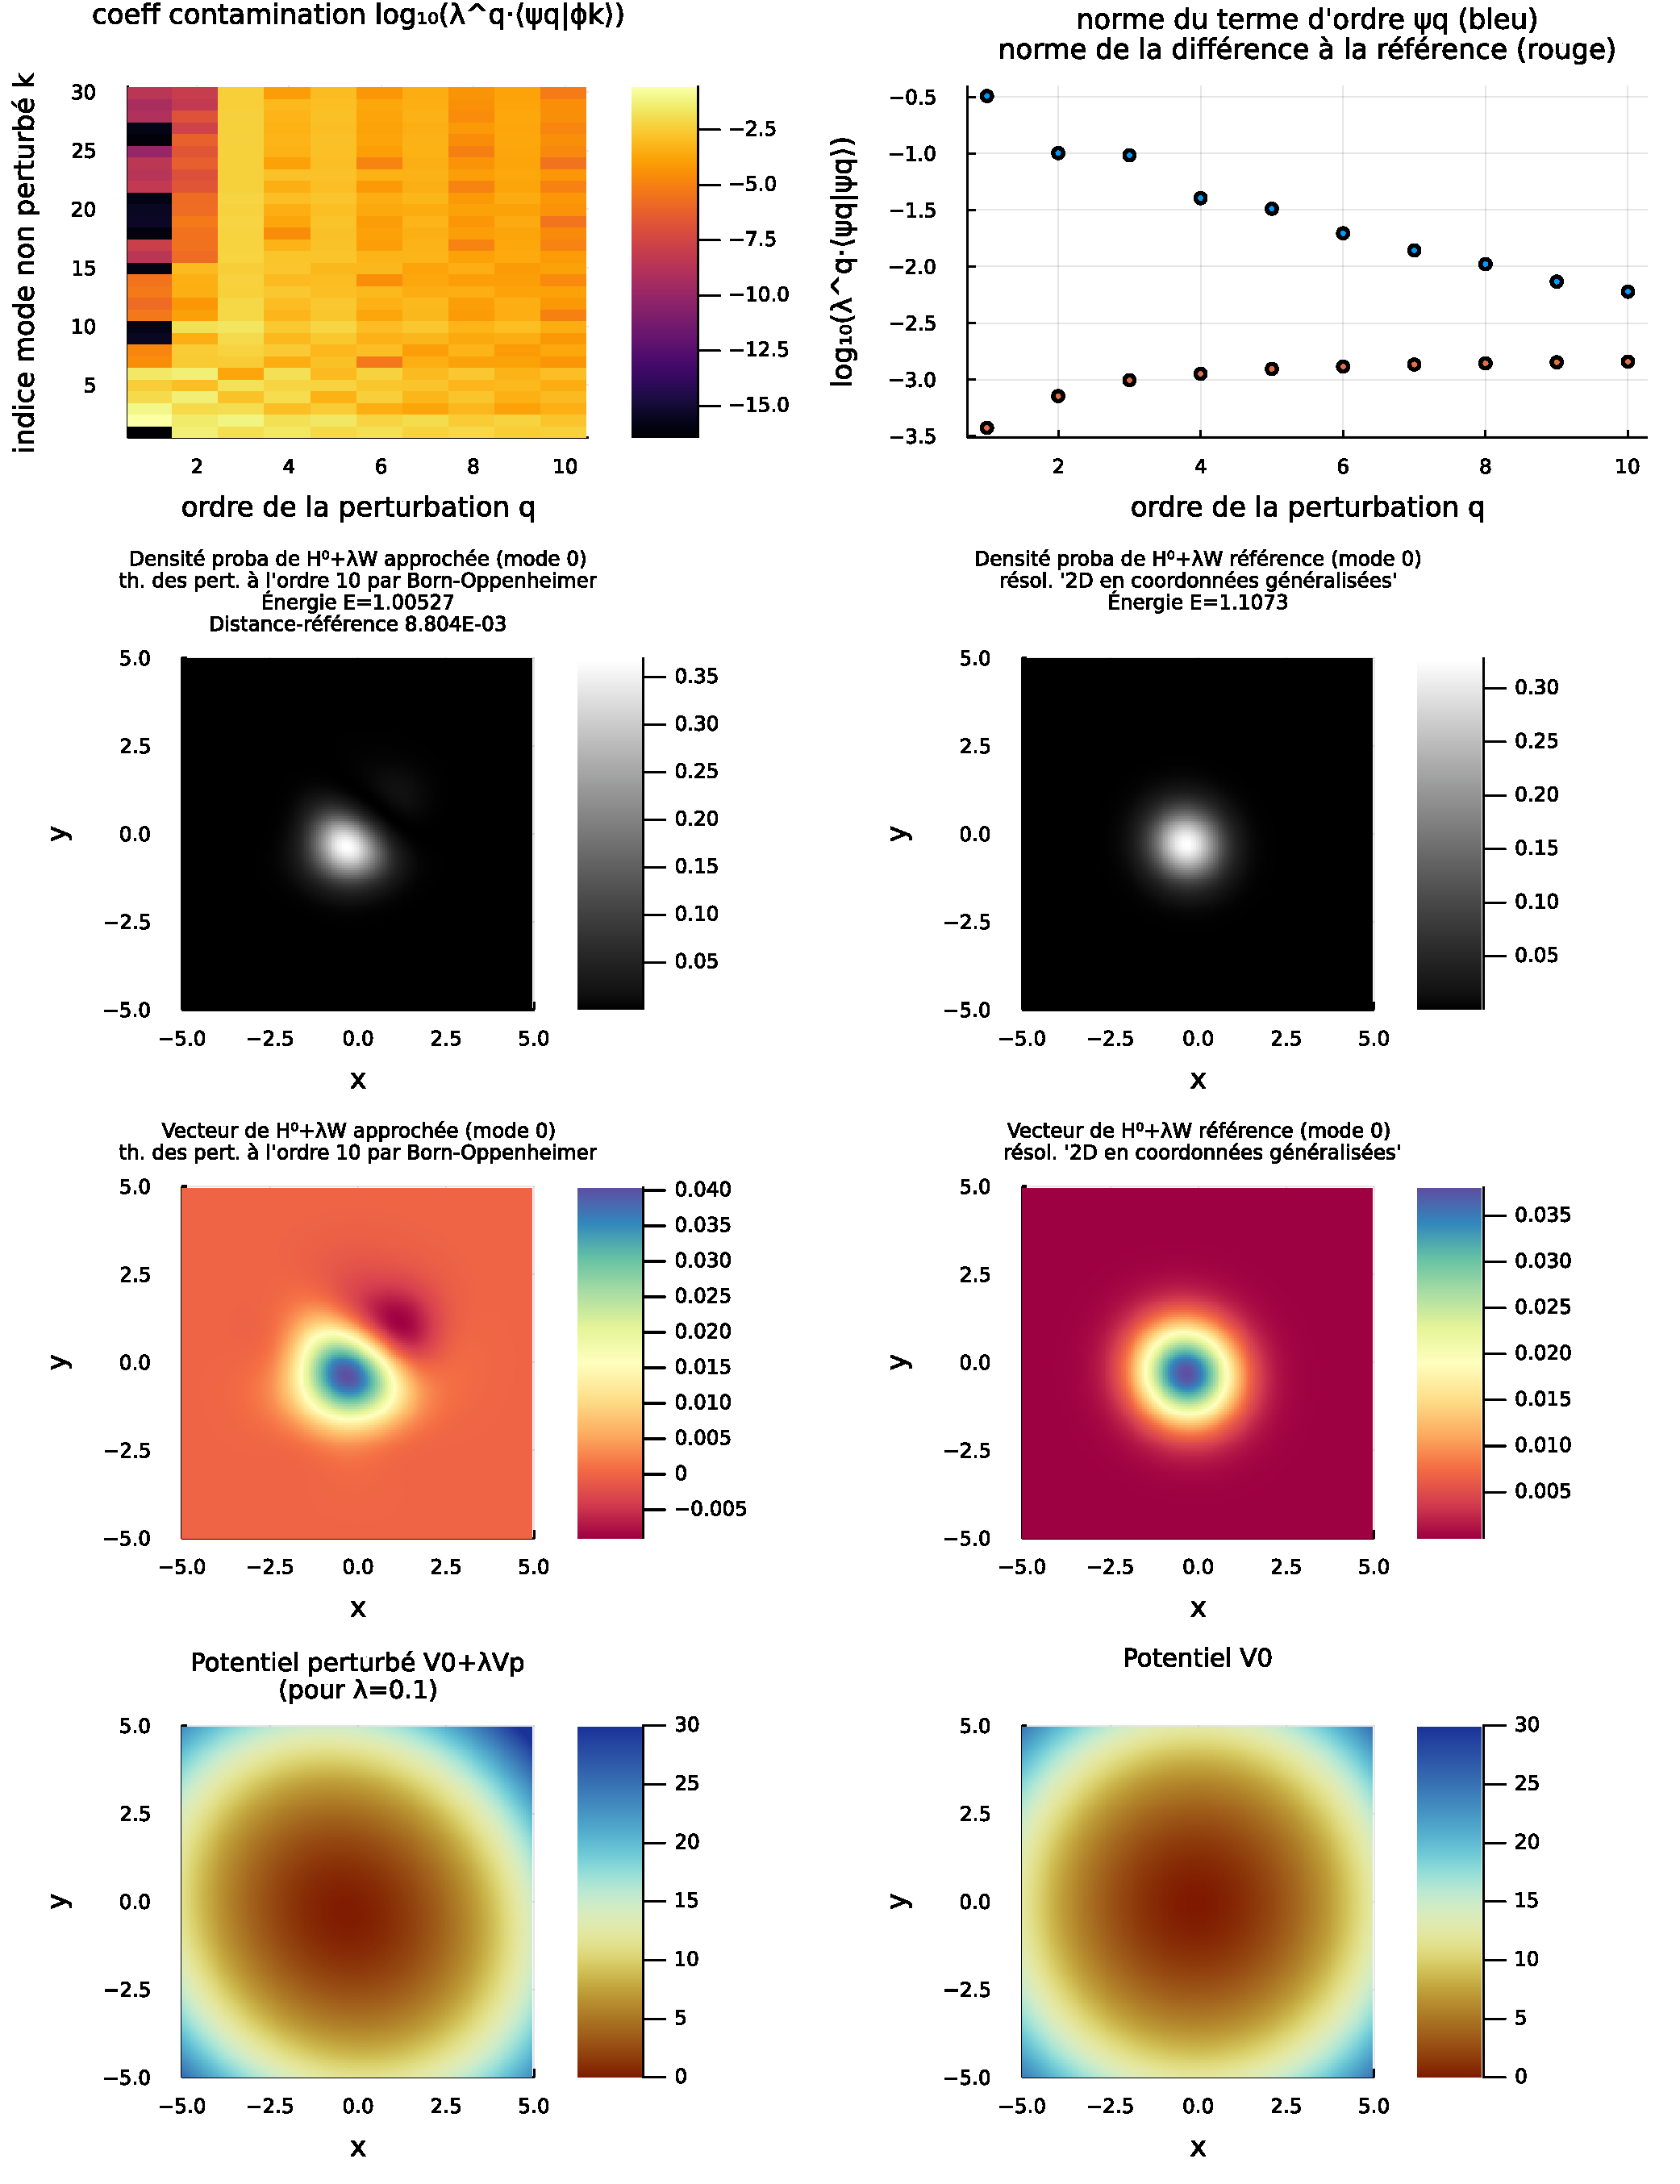
\includegraphics[width=\textwidth]{images/th_pert_exemple.pdf}
    \caption[Résultats de la méthode \textit{sum over states} pour l'OHQ 2D]{Exemple du calcul du mode de l'état fondamental sur l'exemple: oscillateur harmonique 2D, dont la perturbation a été projetée uniquement sur les 30 premiers modes non perturbés par commodité. On constate dans ce cas une convergence mais la meilleure approximation reste l'ordre 1 (voir graphe de la norme à la différence). En clair, ces résultats ne sont pas un franc succès.}
    \label{fig:ex_th_pert}
\end{figure}
    
\subsection{Détermination des termes par projection et descente de gradient}
\label{sec:desc_grad}




\subsubsection{Gradients conjugués}

Explicitons d'abord un résultat avec la méthode des gradients conjugués que l'on présente succintement.
Étant donnée une matrice $A \in \mathscr{S}_m^{++}$ (symétrique positive définie) et un vecteur $\vect{b}$ dans $\mathbb{R}^m$, la méthode des gradients conjugués construit une suite de vecteurs $(\vect{x}^{k})_k$ telle que

\begin{equation*}
    \vect{x}^k \xrightarrow[k \rightarrow + \infty]{} \argmin_{\vect{x}\in\mathbb{R}^m} f(\vect{x}) \coloneqq \vect{x}^\star
\end{equation*}
où $f(\vect{x}) = \frac{1}{2}\vect{x}^\intercal A \vect{x} - \vect{b}^\intercal \vect{x}$, ce qui est donc équivalent à résoudre $A\vect{x} = \vect{b}$.

L'algorithme est présent dans de nombreux ouvrages et références sur internet et se présente de la manière suivante en pseudo-code, que j'ai reproduit ici\footnote{Source: \url{https://en.wikipedia.org/wiki/Conjugate_gradient_method}}:


\begin{align*}
\hbox{Inputs }& \mathbf{x}_0, \mathbf{b}, \mathbf{A} \\
\hbox{Processing } & \mathbf{r}_0 := \mathbf{b} - \mathbf{A x}_0 \\
& \mathbf{p}_0 := \mathbf{r}_0 \\
& k := 0 \\
& \hbox{while } \|\mathbf{r}_k\| \ge \varepsilon \hbox{ do} \\
& \qquad \alpha_k := \frac{\mathbf{r}_k^\mathsf{T} \mathbf{r}_k}{\mathbf{p}_k^\mathsf{T} \mathbf{A p}_k}  \\
& \qquad \mathbf{x}_{k+1} := \mathbf{x}_k + \alpha_k \mathbf{p}_k \\
& \qquad \mathbf{r}_{k+1} := \mathbf{r}_k - \alpha_k \mathbf{A p}_k \\
& \qquad \hbox{if } \|r_{k+1}\| \le \varepsilon \\
& \qquad \qquad  \hbox{return } \mathbf{x}_{k+1} \\
& \qquad \hbox{end if} \\
& \qquad \beta_k := \frac{\mathbf{r}_{k+1}^\mathsf{T} \mathbf{r}_{k+1}}{\mathbf{r}_k^\mathsf{T} \mathbf{r}_k} \\
& \qquad \mathbf{p}_{k+1} := \mathbf{r}_{k+1} + \beta_k \mathbf{p}_k \\
& \qquad k := k + 1 \\
& \hbox{end while} \\
\hbox{Outputs } & \mathbf{x}_{k+1}
\end{align*}

Dans ce code, $\vect{r}$ représente $- \nabla (f)$.

En notant l'erreur $\vect{e}^k = \vect{x}^k-\vect{x}^\star$, cet algorithme a la propriété de vérifier pour tout $k$ \cite{poliak_introduction_1987}:
\begin{equation}
\label{convergence_grad_conj}
    \|\vect{e}^k \| \le 2 \kappa (A) \left( \frac{\sqrt{\kappa (A)} - 1}{\sqrt{\kappa (A)} + 1} \right)^k \| \vect{e}^0\|
\end{equation}

où $\kappa (A)$ désigne le conditionnement de $A$.

Cette méthode présente l'avantage d'être plus rapide asymptotiquement que d'autres algorithmes de résolution de systèmes linéaires comme celui de \textsc{Jacobi} ou \textsc{Gauss-Seidel}, même si elle reste coûteuse en opérations, car il faut faire de nombreux produits matriciels.



\begin{proposition}
Si le vecteur initial $\vect{x}_0$ et $\vect{b}$ appartiennent à un sous-espace $V$ stable par $\vect{A}$, alors la limite s'y trouve également. 
\end{proposition}

\begin{proof}
Montrons que pour tout $k$, $\vect{r}_k$, $\vect{x}_k$ et $\vect{p}_k$ sont dans $V$ avec les hypothèses de la proposition.
On a $\vect{p}_0, \vect{r}_0 \in V$ par combinaison linéaire. Par récurrence, on le suppose vrai à l'indice $k$. Alors en suivant les lignes de l'algorithme, $\vect{x}_{k+1} \in V$ par CL et $\vect{A}\vect{p}_k \in V$ par stabilité, donc par CL et par hypothèse de récurrence, $\vect{r}_{k+1}\in V$. Puis $\vect{p}_{k+1} \in V$ par CL avec $\vect{r}_{k+1}$ et $\vect{p}_k$.

Comme un sous-espace vectoriel de dimension finie est fermé, la limite appartient à $V$, ce qui conclut.
\end{proof}




\begin{proposition}
Dans la base des vecteurs propres $(\phi_1, \cdots, \phi_N)$, de $\hat{H}^0$, la matrice $(\hat{H}^0-E_0)$ s'écrit $\mathrm{diag}(0,E_1-E_0, \cdots, E_N-E_0)$ donc finalement nous avons en notant $\Pi^\perp$ le projecteur orthogonal sur l'orthogonal de $\phi_1$:
\begin{equation}
\label{decomp_sous_esp}
    M = \Pi^\perp (\hat{H}^0-E_0) \Pi^\perp = \renewcommand\arraystretch{2}
\left[
\begin{array}{c|c}
  0 &  0^{N-1}  \\[5pt]
  \hline
  0^{N-1} & R \\[5pt]
\end{array}
\right]
\end{equation}

avec ainsi $\text{Sp}(\hat{H}^0-E_0) = \{0 \} \cup \mathrm{Sp}(R)$ et $\mathrm{Sp}(R) = \{E_1-E_0, \cdots, E_N-E_0\} \subset \mathbb{R}^\star_+$. 


La méthode des gradients conjugués avec $M$ et n'importe quel $\vect{b} \in \mathrm{Vect}(\phi_j)^\intercal$ et $\vect{x}^0=\vect{0}$, aboutit donc  à une solution dans $\mathrm{Vect}(\phi_j)^\intercal$ si le vecteur initial est  $\vect{0}$.



Comme 
\begin{equation}
    \mathbb{R}^N = \mathrm{Vect}(\phi_j)\oplus \underbrace{\mathrm{Vect}(\phi_j)^\perp}_{=\mathrm{Span}(R)  \simeq \mathbb{R}^{N-1}}
\end{equation}
on écrit de manière unique pour tout $\vect{v}\in\mathbb{R}^N, \vect{v}=\vect{v}^k_\parallel + \vect{v}^k_\perp$, et comme d'une part l'orthogonal est stable par $R$, et d'autre part le gradient de $M$ est à valeurs dans cet orthogonal, on obtient que toutes les équations des gradients conjugués valables en remplaçant les vecteurs par leur composante indicée $\perp$. 

Par conséquent, finalement, avec ces vecteurs de départ, on peut  considérer uniquement l'algorithme dans l'hyperplan $\mathrm{Vect}(\phi_j)^\intercal$ et ainsi obtenir la convergence en 

\begin{equation}
    \mathcal{O}\left( \frac{\sqrt{\kappa (R)} - 1}{\sqrt{\kappa (R)} + 1} \right)^k = \mathcal{O}\left( \frac{\sqrt{E_N-E_1} - \sqrt{E_1}}{\sqrt{E_N-E_1} + \sqrt{E_1}} \right)^k
\end{equation} et la limite est bien dans l'orthogonal.
\end{proposition}



Pour éviter l'écueil de devoir connaître les vecteurs propres du hamiltonien non perturbé (ce qui nécessite de diagonaliser le système, on utilise une autre méthode, basée également sur des projections, mais  \textbf{au lieu de calculer exactement chaque projection sur un ensemble limité de vecteurs propres non perturbés, on calcule approximativement (avec une métode itérative) chaque les projections sur deux sous-espaces supplémentaires dont la somme directe recouvre l'espace}, grâce aux gradients conjugués.

Reprenons les formules  du DSE de la perturbation à tout ordre:
\begin{align*}
    (\hat{H}^0-E_0) |\psi_0\rangle &= 0 \, \text{(ordre 0)} \\
    (\hat{H}^0-E_0) |\psi_1\rangle + (\hat{W}-E_1) |\psi_0\rangle &=0 \, \text{(ordre 1)}  \\
    (\hat{H}^0-E_0) |\psi_2\rangle + (\hat{W}-E_1) |\psi_1\rangle - E_2 |\psi_0\rangle &= 0 \, \text{(ordre 2)}  \\
    &\vdots \\
    (\hat{H}^0 - E_0) |\psi_q\rangle + (\hat{W}-E_1)|\psi_{q-1}\rangle -E_2 |\psi_{q-2}\rangle + \dots - E_q |\psi_0\rangle &= 0 \, \text{(ordre $q$)} 
\end{align*}

Comme pour la méthode \textit{sum over states}, on va distinguer des cas, mais seulement deux: projection sur $\mathrm{Vect}(\phi_j)$ (mode que l'on cherche à approcher après perturbation); et $\mathrm{Vect}(\phi_j)^\perp$. Toutes les équations ci-dessus sont en particulier valables sur ces deux sous-espaces vectoriels par linéarité. Notons pour la suite $\Pi^\parallel$ le projecteur orthogonal sur $\mathrm{Vect}(\phi_j)$ et  $\Pi^\perp$ le projecteur sur $ \mathrm{Vect}(\phi_j)^\perp$.

\subsubsection{À l'ordre 1}
On a vu précédemment que $\psi_1 \in \phi_0^\perp$, ce qui permet d'écrire $|\psi_1 \rangle = \Pi^\perp |\psi_1 \rangle$ et  en projetant l'équation d'ordre 1 \ref{ordre1} sur l'orthogonal à gauche il vient:
\begin{equation}
\label{perp_o1}
    \Pi^\perp (\hat{H}^0-E_0) \Pi^\perp |\psi_1\rangle   =-\Pi^\perp \hat{W} |\psi_0\rangle
\end{equation}

Puisque $E_0$ est non dégénérée, l'application linéaire $\Pi^\perp (\hat{H}^0-E_0) \Pi^\perp$ restreinte au sous-espace orthogonal est inversible. On a donc un système linéaire singulier dont seule une direction est nulle. En pratique, on utilise l'algorithme des gradients conjugués avec vecteur initial nul (qui appartient aux deux sous-espaces en somme directe).

On a déjà montré que l'énergie $E_1$ s'obtenait par \ref{en_E1}:
\begin{equation}
\label{en_o1}
    E_1 = \langle \psi_0 | \hat{W} | \psi_0 \rangle
\end{equation}



\subsubsection{À l'ordre $q\ge 2$}

On part de l'ordre $q$ en supposant les $|\psi_i\rangle$ avec $i<q$ connus, et comme précédemment, on exploite le fait que $(\hat{H}^0-E_0)$ laisse stables les sous-espaces supplémentaires ce qui entraîne la commutation $(\hat{H}^0-E_0) \Pi^\perp = \Pi^\perp (\hat{H}^0-E_0)$ et $(\hat{H}^0-E_0) \Pi^\parallel = \Pi^\parallel (\hat{H}^0-E_0)$.

D'abord, nous écrivons

\begin{equation}
\label{s_en1}
    \underbrace{\langle \psi_0 | \hat{H}^0-E_0 |\psi_q\rangle}_{=0} = -\langle \psi_0 | \hat{W}-E_1 |\psi_{q-1}\rangle + \langle \psi_0 |  \sum_{i=0}^{q-2} E_{q-i} |\psi_i\rangle
\end{equation}


Cela permet de trouver l'énergie d'ordre $q$:

\begin{equation}
\label{en_oq}
    E_q =    \langle \psi_0 |\hat{W}-E_1 | \psi_{q-1} \rangle - \sum_{i=1}^{q-2} E_{q-i} \langle \psi_0 |   \psi_{i}\rangle
\end{equation}

Ensuite,  on prend  l'égalité à l'ordre $q$ des termes du DSE  que l'on projette sur l'orthogonal, ce qui fait apparaître le système linéaire suivant pour l'état $|\psi_q \rangle$.

\begin{equation}
\label{s_perp}
    \Pi^\perp (\hat{H}^0-E_0)  \Pi^\perp |\psi_q\rangle = - \Pi^\perp (\hat{W}-E_1) |\psi_{q-1}\rangle +  \Pi^\perp \sum_{i=0}^{q-2} E_{q-i} |\psi_i\rangle
\end{equation}
Tandis que la composante suivant son supplémentaire est donné, comme pour la méthode précédente, par le fait que $|\Psi\rangle$ est normé fà tout ordre: on a alors déjà écrit en \ref{phijpsiq} l'égalité qui nous manque:
\begin{equation}
\label{s_para}
    \| \Pi^\parallel |\psi_q\rangle \| = \langle \psi_0 | \psi_q\rangle=-\frac{1}{2}\sum_{i=1}^{q-1} \langle \psi_i |\psi_{q-i} \rangle 
\end{equation}
On a enfin bien-sûr:
\begin{equation}
    \psi_q = \Pi^\perp \psi_q + \Pi^\parallel \psi_q
\end{equation}


Là encore on se retrouve avec des équations dont la résolution est très facilement automatisables et dont le code sera d'ailleurs très succinct puisque des bibliothèques implémentent les gradients conjugués.




\subsubsection{Complexité asymptotique et implémentation}

À l'origine, une première version de l'algorithme que j'avais programmé mettait en \oe{}uvre cette méthode avec l'usage du GPU de manière naïve (i.e., reprenant les lignes de calcul point par point). C'était l'occasion d'apprendre à maîtriser un nouvel outil. L'algorithme et les hypothèses sont donnés en annexe (algorithme \ref{alg:conj_grad_pert}). Le paradigme principal était alors d'exploiter le GPU pour des calculs lourds (tels que les projections)




    
    Ce choix est mauvais à plusieurs égards à ce stade de la conception:
\begin{itemize}
    \item D'une part il requiert des bibliothèques \og compliquées \fg{} pour piloter les opérations sur GPU et le matériel en lui-même, ce qui peut facilement dégénérer en transferts mémoire longs comme on le verra dans une section ultérieure;
    \item D'autre part les GPU n'ont pas nécessairement des c\oe{}urs rapides à la  précision flottante sur 64 bits.
    \item La plupart des produits coûteux entre matrices et vecteurs peuvent être facilement évités en n'assemblant pas les matrices de projecteurs. 
    \item Certains cas ne sont pas nécessairement implémentés en Julia sur GPU: à l'été 2022, un produit matrice-matrice \texttt{sparse*dense} est supporté par Julia CUDA, mais pas \texttt{dense*sparse}.
    \item Enfin, mes tests ont montré que pour les routines disponibles employables pour résoudre mon problème, la sensibilité aux conditions initiales est grande, on doit donc savoir ce qu'on cherche à l'avance et le temps d'exécution est simplement plus long que sur CPU donc ça n'a pas beaucoup d'intérêt.\footnote{Un intérêt est cependant que l'ordinateur chauffera moins.}
\end{itemize}

J'ai alors plus simplement fait le choix d'en rester aux seuls CPU, sans même aller jusqu'à choisir le GPU pour certaines étapes seulement (cf annexe tout mon travail effectué en section \ref{sec:optim_hardware}).


Quant aux projections, il s'agit d'une instance particulièrement simple du problème de \textbf{parenthésage optimal des multiplications matricielles enchaînées} (dans notre cas, mettant en jeu uniquement des matrices et vecteurs). Plus clairement, pour effectuer le calcul $\Pi \vect{x}$ avec $\Pi$ un projecteur selon un vecteur \emph{normé} connu $\vect{y}$, on ne calcule pas naïvement $(\vect{y} \vect{y}^\intercal) \vect{x}$ (coût $\mathcal{O}(N^2)$), mais plutôt $\vect{y} (\vect{y}^\intercal \vect{x})$ (coût $\mathcal{O}(N)$). Ce calcul ne peut cependant pas être utilisé comme variable classique dans les expressions des calculs courants. Pour utiliser cette décomposition dans des routines telles que les gradients conjugués, on la formalise donc en construisant un objet \codewordblue{LinearMap} avec par exemple la commande \codeword{Π_par  = LinearMap(x -> dot(Ψ,x)*Ψ, N²);}, que l'on peut ensuite appeler comme une fonction via une méthode associée dédiée, ou dans dans les fonctions routines du paquet \codewordred{IterativeSolvers} en Julia, telles que \codewordgreen{cg}. C'est à peu près la seule \og difficulté technique \fg{} posée par ce choix, si on ne veut pas réécrire le code des gradients conjugués entièrement à la main.


Je me propose de montrer dans ce paragraphe que la complexité asymptotique de l'algorithme précédent (utilisant les gradients conjugués) est meilleure que celui basé sur la \emph{sum over states}, sous l'hypothèse que la valeur propre maximale de la matrice du hamiltonien en dimension $N$ tend vers $+\infty$ lorsque $N\rightarrow + \infty$, ce qui est le cas dans le théorème XIII.64 dans \cite{reed_methods_1980}. 


\begin{proposition}
Au voisinage de $N \rightarrow + \infty$ (i.e. pour $N$ suffisamment grand),  la condition 
\begin{equation}
\label{condition_precision_machine}
    k   \ge - \frac{1}{2}\sqrt{\kappa(R)} \left[\ln \varepsilon - \ln (2 \kappa (R) \| \vect{e}^0\|) \right]
\end{equation}
est suffisante pour que la précision machine en précision double (FP64) $\varepsilon \approx 10^{-16}$ soit atteinte lors de l'application des gradients conjugués (rappelons que $R$ est la matrice qui apparaît dans \ref{decomp_sous_esp}).


En d'autres termes, le nombre $k$ d'itérations nécessaires des gradients conjugués est majoré asymptotiquement par
\begin{equation}
    \boxed{k = \mathcal{O}\left( \sqrt{\kappa(R)} \ln \kappa(R)\right)}
\end{equation}
\end{proposition}

\begin{proof}
La condition nécessaire et suffisante sur le nombre d'itérations $k$ pour atteindre la précision machine est (d'après \ref{convergence_grad_conj}) la suivante:


\begin{equation}
\label{condition_convergence_precision_machine}
    2 \kappa (R) \left( \frac{\sqrt{\kappa (R)} - 1}{\sqrt{\kappa (R)} + 1} \right)^k \| \vect{e}^0\| \le \varepsilon \Longleftrightarrow  k \ln \left( \frac{\sqrt{\kappa (R)} - 1}{\sqrt{\kappa (R)} + 1} \right)   \le \ln \varepsilon -  \ln (2 \kappa (R) \| \vect{e}^0\|
\end{equation}

D'autre part on a aussi $\kappa(R)= \frac{E_N-E_0}{E_1-E_0} \xrightarrow[N \rightarrow + \infty]{} +\infty$ (cf. équation \ref{decomp_sous_esp}).

Ainsi, en supposant la matrice $R$ suffisamment grande (donc $N$ suffisamment grand, donc la grille suffisamment fine), les énergies de plus en plus hautes pourront être approchées et le conditionnement de $R$ sera suffisamment grand pour écrire son développement asymptotique au voisinage de $+\infty$: $\frac{\sqrt{x}-1}{\sqrt{x}+1}\underset{+\infty}{=} 1 - \frac{2}{\sqrt{x}}+ \frac{1}{x} + o\left(\frac{1}{x}\right)$ et parvenir à 
\begin{equation*}
     \frac{\sqrt{\kappa (R)} - 1}{\sqrt{\kappa (R)} + 1}  \le 1-\frac{2}{\sqrt{\kappa (R)}} + \frac{1}{(\kappa (R))^{3/2}}
\end{equation*}




Or, un développement limité (ou un rapide calcul automatisé dans \href{https://pari.math.u-bordeaux.fr/}{PARI/gp} pour la vérifiabilité) permet d'obtenir au voisinage de 0: $\ln (1-2x + x^3) \underset{x\rightarrow 0}{=}-2x-2x^2+o(x^2) \underset{x\rightarrow 0}{\le} -2x$ donc lorsque $\kappa(R)$ est grand:
\begin{equation*}
   \ln \left(1-\frac{2}{\sqrt{\kappa (R)}} + \frac{1}{(\kappa (R))^{3/2}} \right) \le - \frac{2}{\sqrt{\kappa (R)}}
\end{equation*}

Par conséquent, la condition \ref{condition_precision_machine} implique vérifiée la chaîne d'inégalités suivantes pour $\kappa(R)$ grand (en partant de la droite):

\begin{equation*}
    k\ln \left( \frac{\sqrt{\kappa (R)} - 1}{\sqrt{\kappa (R)} + 1} \right) \le k\ln \left(1-\frac{2}{\sqrt{\kappa (R)}} + \frac{1}{(\kappa (R))^{3/2}} \right) \le - \frac{2k}{\sqrt{\kappa (R)}} \le \ln \varepsilon - \ln (2 \kappa (R) \| \vect{e}^0\|) 
\end{equation*}
En ignorant les inégalités intermédiaires on obtient \ref{condition_convergence_precision_machine}, ce qui conclut.

\end{proof}







%\begin{multline}
     %- \frac{2k}{\sqrt{\kappa (R)}}  \le \left[\ln \varepsilon - \ln (2 \kappa (R) \| \vect{e}^0\|) \right] \\ \Longrightarrow \ln \left(1-\frac{2}{\sqrt{\kappa (R)}} + \frac{1}{(\kappa (R))^{3/2}} \right) \le \left[\ln \varepsilon - \ln (2 \kappa (R) \| \vect{e}^0\|) \right] \\
    %\Longrightarrow \ln \left( \frac{\sqrt{\kappa (R)} - 1}{\sqrt{\kappa (R)} + 1} \right)  \le \left[\ln \varepsilon - \ln (2 \kappa (R) \| \vect{e}^0\|) \right]
%\end{multline}


\subsubsection{Complexité de la méthode complète}

Dénombrons alors les opérations (produits, divisions) coûteuses pour parvenir à la solution jusqu'à l'ordre $Q_\text{max}$:


\begin{itemize}
    \item Les opérations dans le terme de droite (RHS)\footnote{Right-Hand Side} de \ref{perp_o1} comptabilisent $3N$ produits exactement, puisque $\hat{W}$ est diagonale. Chaque application de l'opérateur du terme de gauche (LHS)\footnote{Left-Hand Side} de \ref{perp_o1}, comptabilise au plus $10N$ produits. En effet, c'est sans assembler $\hat{H}^0-E_0$ (pire cas), et en prenant en compte les projections non assemblées ($2N$ produits chacune) et le fait que $\hat{H}^0$ est creux (laplacien à 5 points). On a donc bien pour $\Pi^\perp (\hat{H}^0-E_0) \Pi^\perp |\psi_1\rangle$, le total $2+(5+1)+2 = 10$.
    
    \item Le calcul de \ref{en_o1} comprend exactement $2N$ produits.
    
    \item Le calcul de \ref{en_oq} comprend exactement $3N+(q-2)(N+1)=(q+1)N+q-2$ produits.
    \item Le terme RHS de \ref{s_perp} s'effectue en $4N+(2(q-1)+1)N=(2q+3)N$ produits. Chaque application de l'opérateur du LHS s'effectue comme vu précédemment en $10N$ produits.
    \item Enfin, le calcul du coefficient cherché dans \ref{s_para} met en jeu  $qN$ produits.
    %\item Les 6 produits matrice-matrice dans le calcul des opérateurs $\Pi^{\perp,\parallel} (\hat{H}^0-E_0)\Pi^{\perp,\parallel}$ et $\Pi^{\perp,\parallel} (\hat{W}-E_1)$  est a priori coûteux, même s'il  s'effectue  une fois pour toutes. Avec l'algorithme naïf, il requiert  $\mathcal{O}(N^3)$ opérations (exactement $N^3$ produits de FP64 pour chaque produit matriciel). En informatique théorique, on connaît des algorithmes de complexité inférieure (notamment, algorithme de \textsc{Strassen}, en $\mathcal{O}(n^{2.8073})$), mais ces algorithmes sont de fait peu utilisés en raison de nombreux problèmes. On peut en citer deux pour \textsc{Strassen}: (i) l'optimalité ne commence à être significative que pour des matrices de très grande taille (plusieurs milliers ou dizaines de milliers de dimensions, ce qui est toutefois atteignable si l'on discrétise finement) et seulement sur certaines architectures matérielles, et (ii) la stabilité numérique de celui-ci est pire que l'algorithme classique. Pour les besoins de la preuve et montrer que cet algorithme est théoriquement un peu meilleur que le précédent, je prendrai en compte la complexité de \textsc{Strassen}\footnote{Car l'algorithme est simple et compréhensible par quiconque connaît l'algèbre linéaire de CPGE en France, ou \emph{Algebra I} dans les pays anglosaxons.} pour éluder ce calcul en particulier mais en pratique, on gagne bien plus à paralléliser massivement (i.e., sur GPU ou CPU), ce qui améliore considérablement la complexité en temps sans changer celle en opérations, mais rend  cette étape de l'algorithme de difficulté dérisoire et ne présente pas le c\oe{}ur du problème que l'on tente de résoudre avec cette approche. 
    
   
    %\item Le calcul des paramètres (membres de gauche dans \ref{s_perp} et \ref{s_para}) à chaque ordre $q\ge 2$ requiert stricto sensu  $(q-1)N+N^2$ produits et l'ordre 1, seulement $N^2$  (membre de gauche dans \ref{perp_o1}).
    
    %\item Calculer $\langle \psi_0 | \hat{H}^0-E_0 | + \langle \psi_0 |\hat{W}-E_1 |$ qui s'effectue une fois pour toutes en $2(N^2+N)$ produits.
    
    %\item Ceci étant donné, le calcul de $E_q$ (éq. \ref{s_en}) consiste donc en $q$ produits matriciels vecteur-vecteur requérant chacun $N$ produits. 
    
    %\item Chaque itération des gradients conjugués opère un nombre de multiplications/divisions en $\mathcal{O}(N^2)$ seulement (multiplications matrice-vecteur, produits scalaires et divisions de réels).
\end{itemize}

 

Ainsi donc le coût total asymptotique de la méthode jusqu'à l'ordre $Q_\text{max}$ pour obtenir la limite à la précision machine est donné par 
\begin{equation}
    %\underbrace{\mathcal{O}(N^{2.8073})}_{\text{calcul opérateurs}} +
    \underbrace{10N+\mathcal{O}\left(N\sqrt{\kappa(R)} \ln \kappa (R)\right)}_{q=1} + \sum_{q=2}^{Q_\text{max}} \left[(q+1)N+q-2 +\mathcal{O}\left(N\sqrt{\kappa(R)} \ln \kappa (R)\right) +qN \right]
\end{equation}

\begin{minted}[
frame=lines,
framesep=2mm,
baselinestretch=1,
fontsize=\small,
breaklines=true,
linenos=false,
bgcolor=white,
escapeinside=||,
mathescape=true]{python}
N, q, c, Q = var('N, q, c, Q')
10*N+c*N+sum((q+1)*N+q-2+c*N+q*N, q,2,Q).simplify()
\end{minted}



Asymptotiquement, on aboutit à un nombre de produits qui croît comme:
\begin{equation}
    \boxed{\mathcal{O}(NQ_\text{max}^2)+\mathcal{O}\left(+NQ_\text{max}\sqrt{\kappa(R)} \ln \kappa(R) \right) }
\end{equation}


\begin{remark}
Vis-à-vis de la grille, on a donc grandement amélioré en pratique la complexité de l'algorithme précédent (qui était en $\mathcal{O}(N^3 Q_\text{max})$).

La clé est de décomposer le problème sur deux sous-espaces seulement (au lieu de $N$ sous-espaces propres précédemment) en utilisant avantageusement des méthodes à convergence géométrique pour résoudre de manière les systèmes linéaires nécessaires.

En pratique cependant, comme le paramètre déterminant est $N$ (en effet, vu que les constantes devant les termes sont asymptotiques comparables, l'ordre de perturbation $Q_\text{max}$ restera en fait majoré et n'a aucune chance de frôler les mêmes ordres de grandeur que $N$), la complexité se réduit donc à
\begin{equation}
    \mathcal{O}\left(N\sqrt{\kappa(R)} \ln \kappa(R) \right)
\end{equation}

Pour une grille de taille $N=n \times n$ d'étendue fixée avec $\kappa(R)= \frac{E_N-E_0}{E_1-E_0}$, on a donc $\mathcal{O}\left(n^2 \sqrt{E_\text{max}(n)} \ln(E_\text{max}(n)) \right)$.  Il resterait à déterminer la croissance des énergies propres approchées en fonction de la taille de la grille pour obtenir une expression dépendant uniquement de $n$.
\end{remark}



\subsection{Application à l'ion $H_2^+$}

\subsubsection{Résumé de la procédure}

Pour résumer, récapitulons les points importants de notre algorithme d'approche de l'état fondamental:
\begin{enumerate}
    \item Choisir une famille de  fonctions de potentiel et choisir les paramètres de sorte qu'à $R$ fixé, le hamiltonien de l'électron ne possède qu'une ou deux valeurs propres négatives, et choisir les paramètres de masse (\S\ref{sec:choix_fonctions});
    \item Évaluer l'argument minimisant l'énergie de surface $R_0$ (\S\ref{sec:minimum_R}) et évaluer numériquement $\frac{\mathrm{d}^2E}{\mathrm{d}\lambda^2}$ (avec un noyau de différences finies par exemple);
    \item Calculer un développement limité du potentiel en espace suivant la direction autour de $R_0$  (\S\ref{sec:chgt_var_adim});
    \item Calculer suivant chaque axe les états fondamentaux mutuellement découplés par n'importe quelle méthode connue en analyse numérique (\S \ref{generalites_elt_analyse_num}) ce qu'on suppose savoir faire car la taille des données reste selon chaque axe comparativement petite;
    \item Perturber le produit tensoriel (loi produit) de ces états à l'aide de l'algorithme des perturbations et des termes du DL précédent (\S\ref{sec:desc_grad});
\end{enumerate}


On calcule donc numériquement le potentiel perturbateur tronqué \ref{W_pert_tronque} du potentiel de l'ion $H_2^+$ que l'on a calculé (éq.  \ref{potentiel_H2plus}) avec les paramètres $\beta=1.5, \eta=0.5, V_0 = 1.5, \sigma = 1$, $m_e = 1, m_p \in [10^1,+\infty[$ comme déjà donnés plus haut.

Les figures qui suivent donnent une visualisation des résultats de la procédure entière décrite précédemment. \textbf{J'ai pris volontairement pour les graphes une masse très petite de proton afin de montrer l'approche HBO par rapport à la référence.}

\begin{figure}[H]
    \centering
    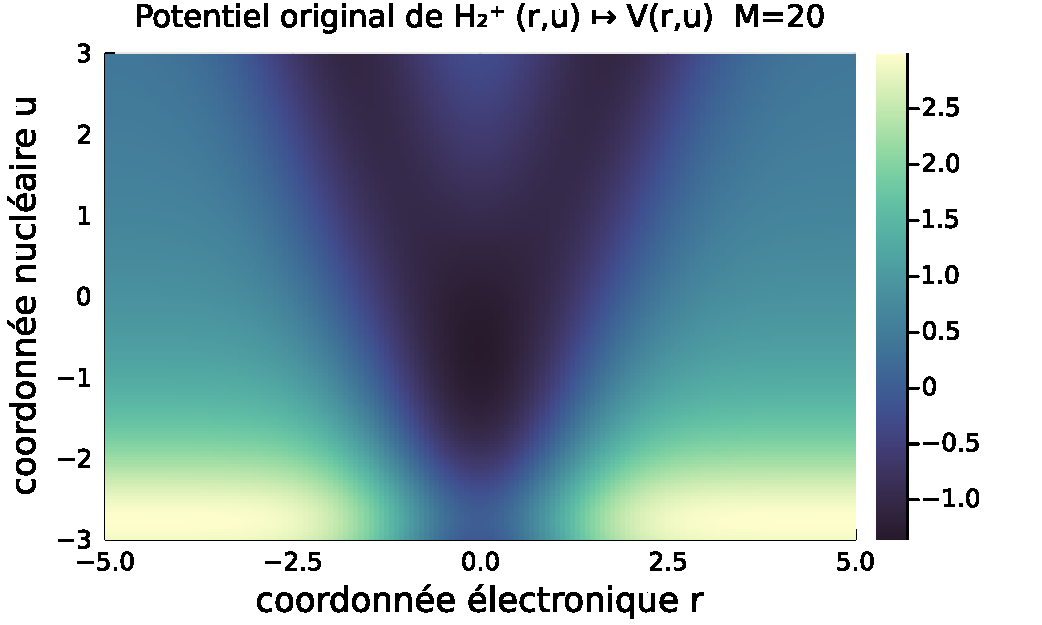
\includegraphics[width=.7\textwidth]{images/formes_résol_H2+/potentiel_original.pdf}
    \caption{Potentiel original de $H_2^+$}
    \label{fig:pot_orig_h2plus}
\end{figure}


\begin{figure}[H]
    \centering
    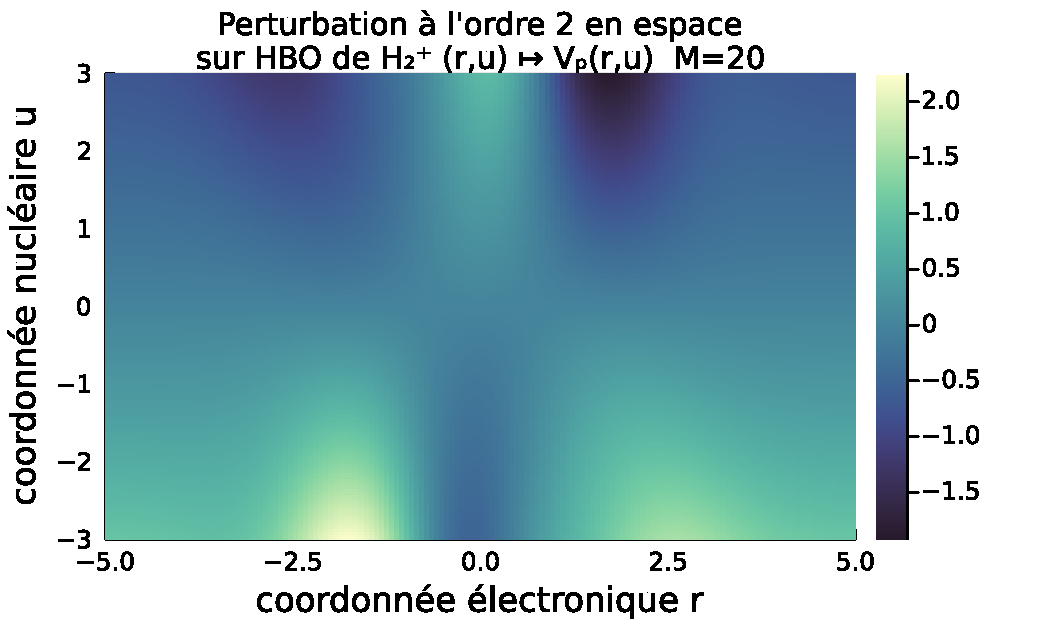
\includegraphics[width=.7\textwidth]{images/formes_résol_H2+/potentiel_pert.pdf}
    \caption{Perturbation du potentiel HBO de $H_2^+$}
    \label{fig:pert_hbo_h2plus}
\end{figure}

\begin{figure}[H]
    \centering
    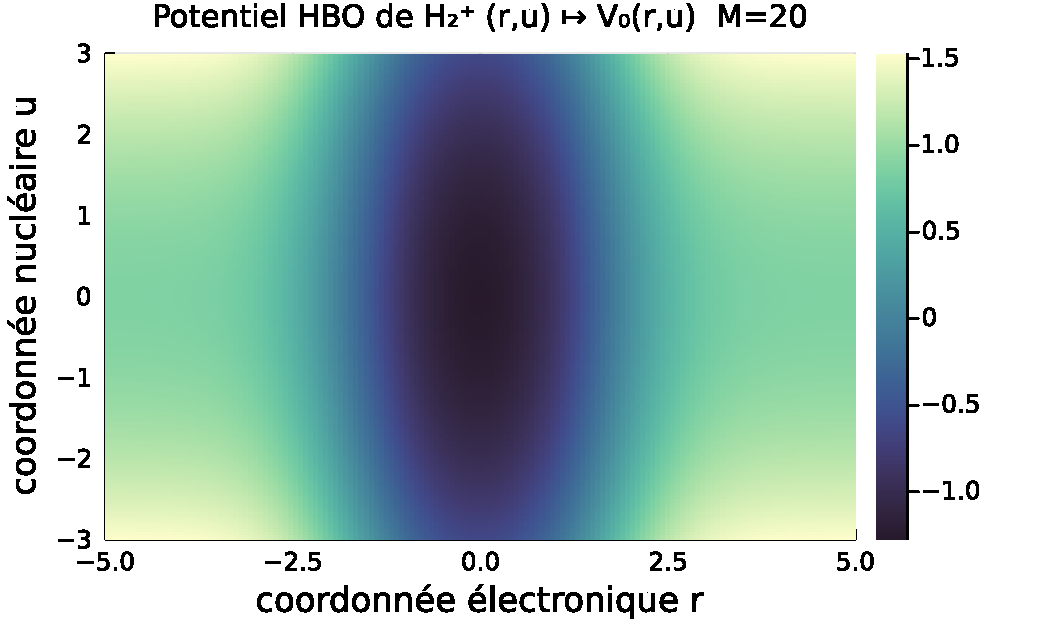
\includegraphics[width=.7\textwidth]{images/formes_résol_H2+/potentiel_HBO.pdf}
    \caption{Potentiel HBO de $H_2^+$, comme vu dans les équations, localement assimilable à un OHQ2D.}
    \label{fig:pot_hbo_h2plus}
\end{figure}

\begin{figure}[H]
    \centering
    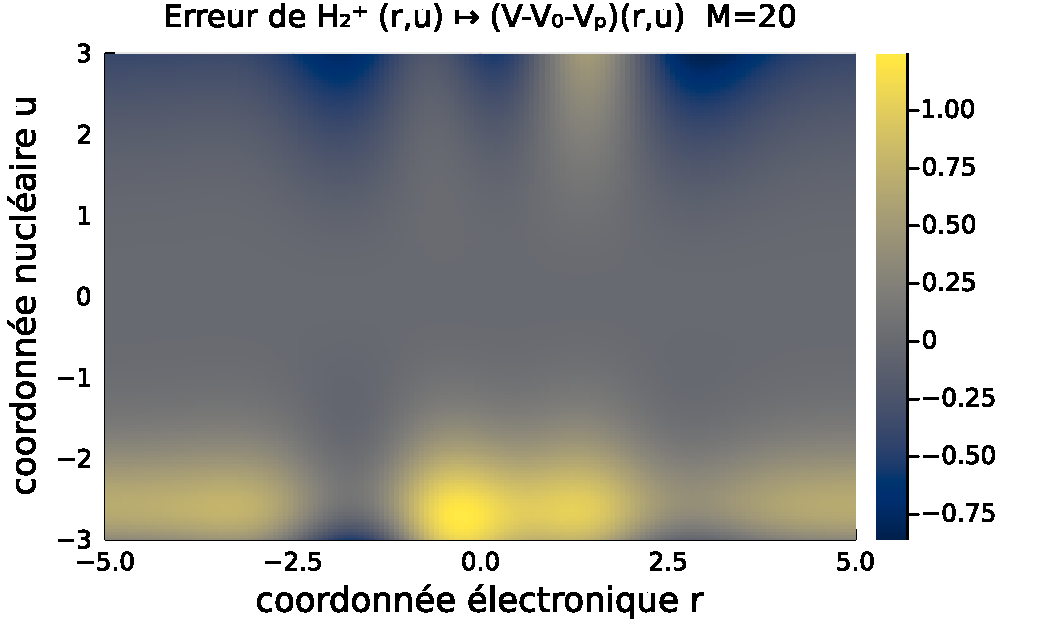
\includegraphics[width=.7\textwidth]{images/formes_résol_H2+/potentiel_erreur.pdf}
    \caption[Erreur commise sur le potentiel original]{Erreur commise sur le potentiel original avec la perturbation. Comme attendu, là où se concentre la probabilité de présence la plus forte, l'erreur est quasi-nulle. On s'attend donc à ce que l'état calculé avec perturbation, soit lui-même proche de la référence.}
    \label{fig:err_hbo_h2plus}
\end{figure}



\begin{figure}[H]
    \centering
    \makebox[\textwidth][c]{\subfloat[\centering densité]{{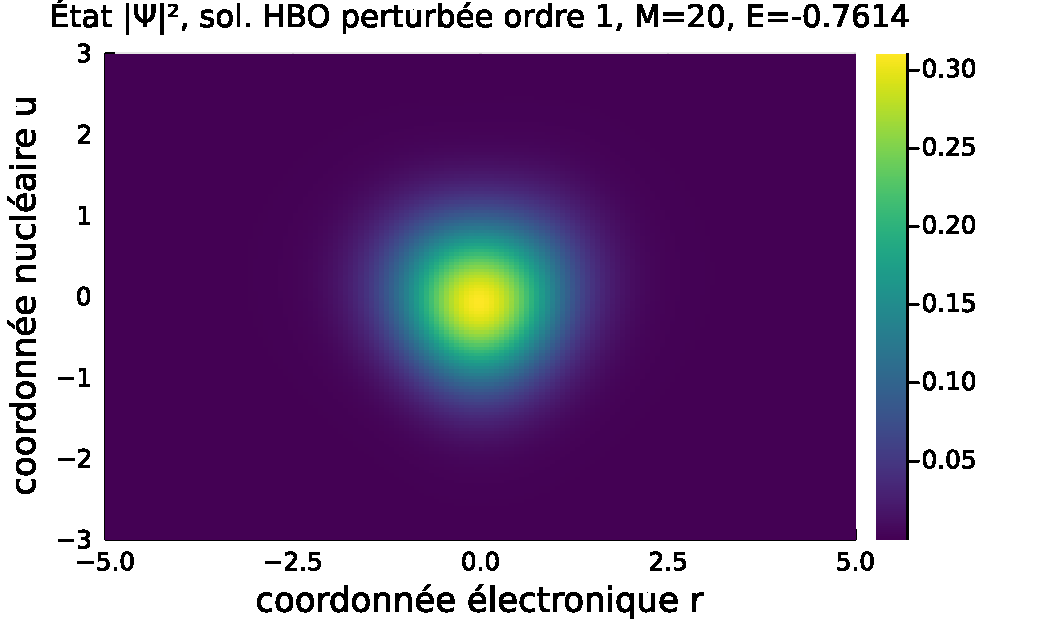
\includegraphics[width=.55\textwidth]{images/formes_résol_H2+/sol_Psi_pert.pdf} }}% https://tex.stackexchange.com/questions/16582/center-figure-that-is-wider-than-textwidth et https://tex.stackexchange.com/questions/37581/latex-figures-side-by-side
    \subfloat[\centering contour]{{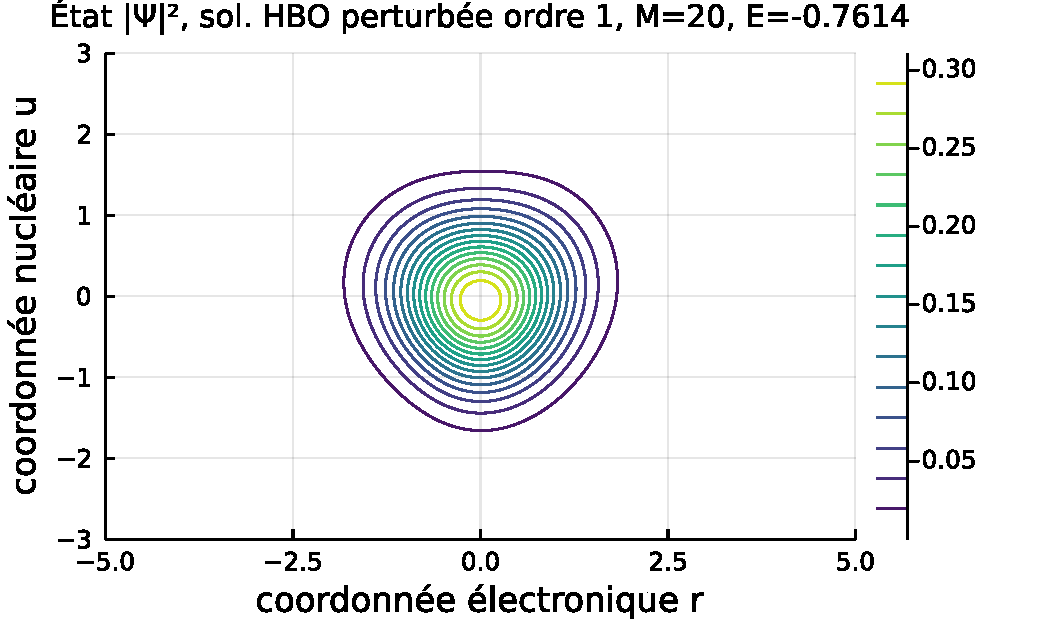
\includegraphics[width=.55\textwidth]{images/formes_résol_H2+/sol_Psi_pert_ct.pdf} }}}
    \caption{Solution HBO approchée par les gradients conjugués à l'ordre 1 en espace}%
    \label{fig:sol_Psi_pert}%
\end{figure}



\begin{figure}[H]
    \centering
    \makebox[\textwidth][c]{\subfloat[\centering densité]{{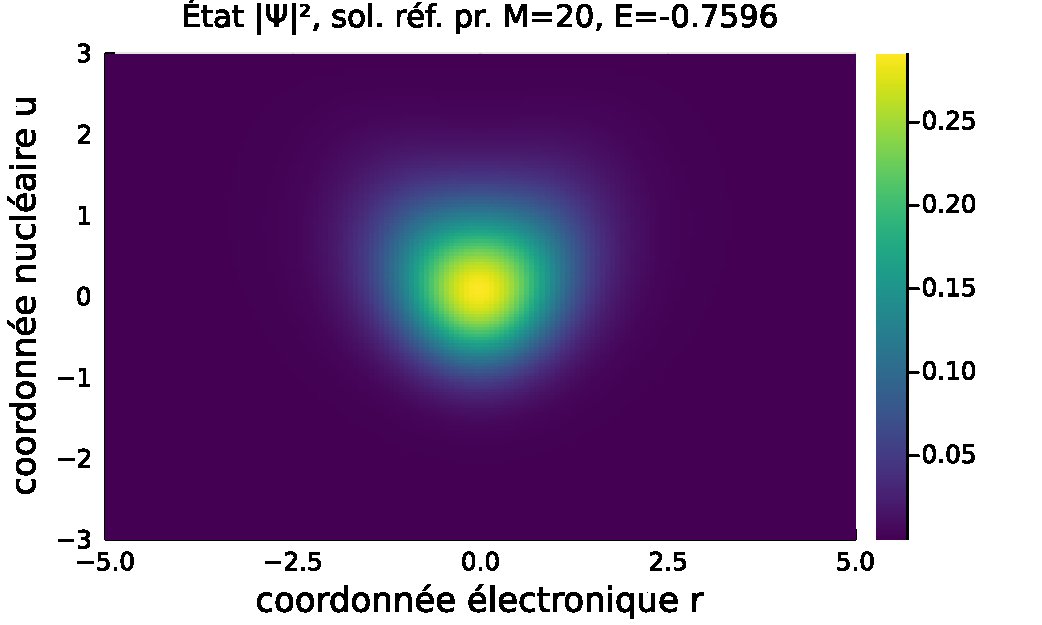
\includegraphics[width=.55\textwidth]{images/formes_résol_H2+/sol_Psi_true.pdf} }}% https://tex.stackexchange.com/questions/16582/center-figure-that-is-wider-than-textwidth et https://tex.stackexchange.com/questions/37581/latex-figures-side-by-side
    \subfloat[\centering contour]{{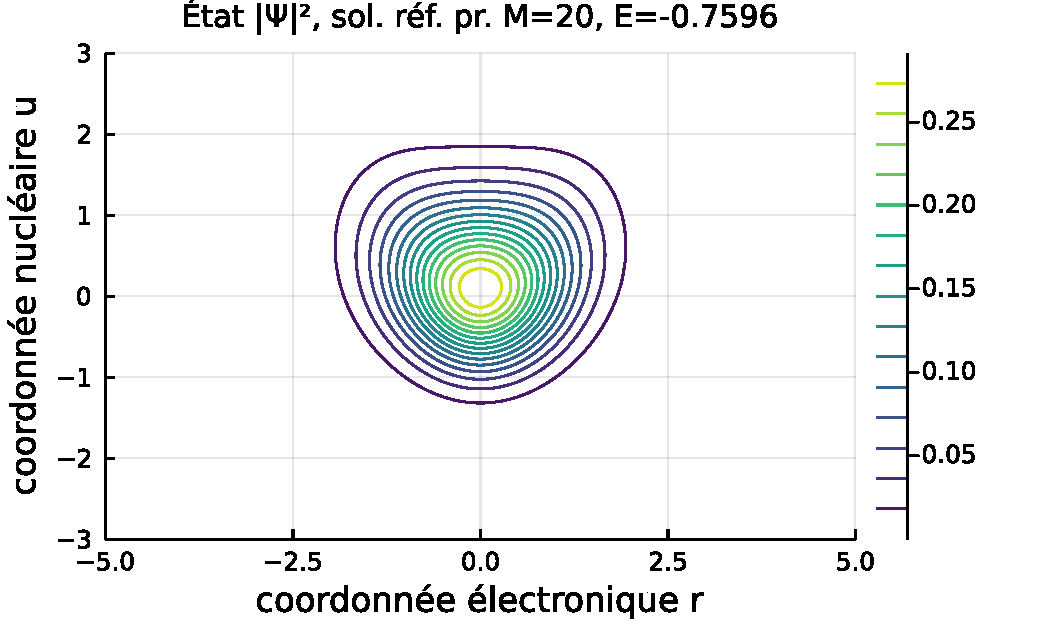
\includegraphics[width=.55\textwidth]{images/formes_résol_H2+/sol_Psi_true_ct.pdf} }}}
    \caption{Solution de référence, calculée en 2D (en trichant) par une méthode de \textsc{Krylov}}%
    \label{fig:sol_Psi_true}%
\end{figure}




\section{Métriques d'évaluation et critique des résultats}


\subsection{Métriques d'évaluation}
\paragraph{Notations de ce paragraphe}
En reprenant les paramètres du problème, on a l'énergie fondamentale vraie $\mathcal{E}_0$ associée à l'état vrai $\psi_0$ ainsi que l'énergie fondamentale approchée par l'algorithme $E_0$ associée à l'état $\Psi_0$ obtenu par perturbation de $\Psi^{\text{HBO}}$.

\subsubsection{Inégalité de \textsc{Kato-Temple}}
 On va appliquer l'inégalité de \textsc{Kato-Temple} \ref{kato_temple_inqeuality}  à l'état fondamental $\psi_0$ trouvé par les perturbations avec \ref{3termes_bis}, en approchant le dénominateur par $K\varepsilon^2$. En effet, on postule que l'énergie de niveau 1 (la plus petite énergie propre strictement supérieure à l'énergie fondamentale est proche de l'énergie caractéristique de l'oscillateur harmonique quantique de $\frak{h}_u$ dans \ref{3termes_bis} (phonon, ou mode de vibration des noyaux) en raison de l'hypothèse de masse électronique très petite $m \ll M$ dans le hamiltonien de départ \ref{hamiltonien_original}, et que par conséquent la contribution en énergie de celui-ci est négligeable devant celle des noyaux. Cette approximation étant de plus en plus valide à mesure que $\frac{m}{M} \rightarrow 0$, i.e. à mesure que $\varepsilon = (MK)^{-\frac{1}{4}} \rightarrow 0$ avec $m=1$ fixé et $M\rightarrow + \infty$. \textbf{Autrement dit, dans ce raisonnement, on considère les deux hamiltoniens totalement découplés pour estimer le gap $\mathcal{E}_1-\mathcal{E}_0$ (énergies véritables) du système total par $E_1-E_0$ (énergies obtenues par perturbations), lui-même estimé par $K\varepsilon^2$.} Cette hypothèse a été testée numériquement avant de l'injecter dans \textsc{Kato-Temple}, et il s'avère que l'erreur relative commise sur le gap est inférieure à 1\textperthousand, ce qui est tout-à-fait satisfaisant pour n'avoir pas à calculer un nouvel état.


Ensuite, on compare les quantités $|\mathcal{E}_1-E_1|$ et $\frac{\|\frak{h}\Psi_0 -  \langle \Psi_0 | \frak{h} | \Psi_0 \rangle \Psi_0 \| }{K\varepsilon^2}$
(notations reprises de \ref{3termes_bis}, $\frak{h}=-\frac{K\varepsilon^2}{2}\frac{\partial^2}{\partial u^2} - \frac{1}{2m} \frac{\partial^2}{\partial x^2} + V(x, R_0+\varepsilon u)$) et on s'attend à avoir l'explication
\begin{equation}
    |\mathcal{E}_0-E_0| \le \frac{\|\frak{h}\Psi_0 -  \langle \Psi_0 | \frak{h} | \Psi_0 \rangle \Psi_0 \| }{K\varepsilon^2}
\end{equation}
Et le but du jeu étant de savoir si l'information contenue dans la majoration est utile ou pas.


\subsubsection{Calcul des erreurs à la référence}
En plus de cela, nous calculons 
\begin{itemize}
\item une norme d'erreur à la solution de référence (qui est donc le vecteur $\Psi_0$ véritable en norme 2 et norme H1 (norme d'espace de \textsc{Sololev}):
\begin{equation}
    \|\underbrace{\psi_0}_{\text{véritable}}-\underbrace{\Psi_0}_{\text{perturbé}}\|
\end{equation} obtenu par résolution 2D de la grille, ce qui serait normalement inaccessible, notre étude visant à ne pas y recourir).
Nous calculons également le résidu simple de la solution perturbée 
\begin{equation}
    \|\frak{h}\Psi_0 -  E_0 \Psi_0 \| 
\end{equation}

\item aussi bien-sûr l'erreur sur l'énergie (la valeur propre):
\begin{equation}
    |\underbrace{\mathcal{E}_0}_{\text{véritable}}-\underbrace{E_0}_{\text{perturbée}}|
\end{equation}
\end{itemize}
Les résultats pour plusieurs masses ont été consignés dans la figure \ref{fig:resultats_simu}.
\begin{figure}[H]
    \centering
    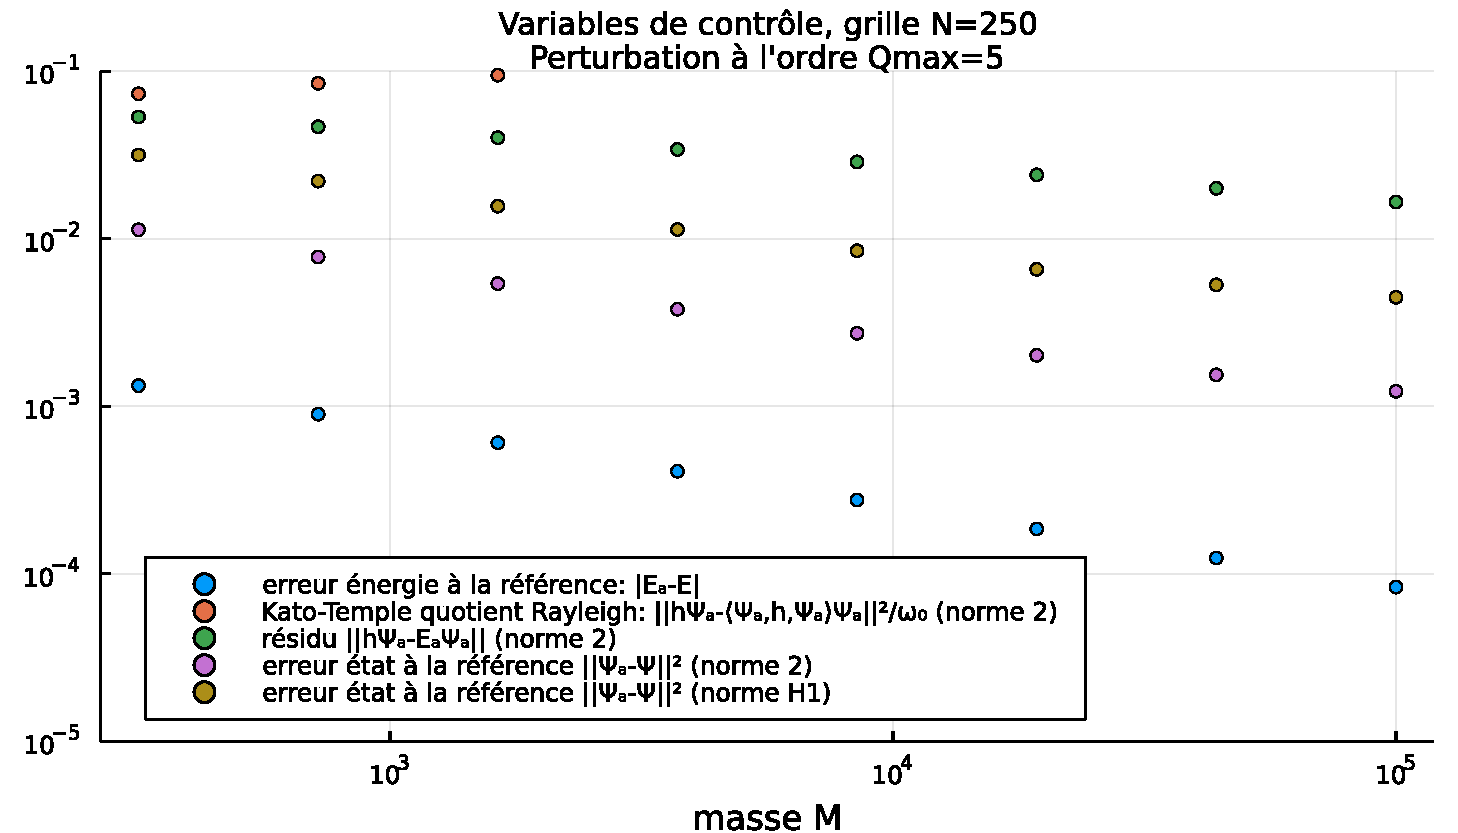
\includegraphics[width=\textwidth]{images/résultats.pdf}
    \caption{Résultats des simulations pour les métriques décrites}
    \label{fig:resultats_simu}
\end{figure}




\subsection{Critique des résultats}
Normalement, le  travail effectué pendant ce stage d'application avec les codes permettrait de guider le travail de recherche pour trouver une explication analytique faite par Éric Cancès et Paul Cazeaux. On a donc approché le problème expérimentalement d'abord, ce qui suit la démarche de la physique. Le travail présentement effectué est donc une bonne base pour de futurs travaux.

\section{Conclusion}
Dans tout le travail présenté, j'ai mis en pratique la méthode d'approximation physique qui m'a été prescrite pour approcher l'état et l'énergie propre d'un système moléculaire simplifié, à savoir $H_2^+$ unidimensionnel. En utilisant Julia, un langage adapté au calcul scientifique, j'ai pu programmer sans encombre l'algorithme à l'aide de quelques considération mathématiques annexes qui permettent d'accélérer et simplifier certaines étapes. À ma connaissance, comparer les résultats aux métriques était une idée originale de mon tuteur scientifique, ce qui devrait permettre de donner un éclairage sur la convergence de telles méthodes à l'avenir pour la communauté de scientifiques en chimie quantique et domaines proches.

\subsubsection{Ouverture}
Dans ce domaine (la chimie quantique et même plus généralement, l'étude des molécules, des protéines du vivant en biologie, etc), comme je l'ai déjà brièvement évoqué, on assiste également à une forte intervention du Machine Learning pour aider à résoudre plus efficacement des problèmes moléculaires (citons par exemple le programme AlphaFold de Google, qui calcule le repliement de protéines, très similaire à ce que l'on fait ici). Cela pourrait donc constituer encore une prolongation au sujet d'étude.




\chapter{Le stage d’application dans le processus de construction du projet professionnel}
\section{Pourquoi ce stage d’application ?}
J'ai choisi ce stage d'application car il répondait parfaitement à mes attentes, à savoir appliquer l'usage de l'informatique et plus précisément, la programmation et la conception d'algorithmes, à un problème ouvert de physique, et plus précisément, de modélisation et de simulation du réel qui puisse avoir des retentissements utiles pour la recherche comme on l'a expliqué dans l'introduction. 

En outre, l'aspect recherche du stage a largement participé à ma décision de candidater. Jusqu'alors à Centrale Lyon, ma formation complémentaire en informatique était uniquement basée sur le Projet Application recherche (PAr), sur les réseaux de neurones appliqués au traitement du langage naturel. M'intégrer le temps du stage à un laboratoire de recherche, discuter avec les chercheurs et doctorants dans le domaine de la chimie quantique s'est révélé particulièrement retentissant vis-à-vis du PAr. J'ai pu également comprendre le fonctionnement d'une unité de recherche et la manière qu'ont les chercheurs de travailler  entre eux.


J'ai pu ainsi apprendre un nouveau langage en devenir (Julia), et améliorer mes connaissances en algorithmique appliquée à l'analyse numérique, dans un cadre où les théorèmes génériques ne sont pas nécessairement applicables et où l'ampleur du problème  force indéniablement à trouver de meilleurs solutions que les algorithmes naïfs qui deviennent vite impraticables.

\section{Profitabilité du stage au projet professionnel}

\subsection{Expérience d'un travail orienté recherche}
De plus, avoir une expérience orientée recherche (qui a en réalité davantage consisté en conception d'algorithmes et adaptation d'un problème exprimé à l'origine en mathématiques et en physique) est pour un ingénieur, je pense, largement valorisable compte tenu des compétences en résolution de problèmes, en autonomie dans l'apprentissage des méthodes sous-jacentes utilisées, etc.

En discutant avec certains camarades de promotion de leur propre stage d'application, j'ai pu me rendre compte que ce sujet proposé au CERMICS était \emph{vraiment} intéressant, ce qui est loin d'être toujours acquis pour des stages orientés programmation et codage à ce niveau d'études et de cette durée. Et pour cause, il y avait réellement de \emph{tout} dans le sujet: de la physique et de la chimie au niveau de la formulation et des enjeux, des mathématiques au niveau de la formalisation sur lesquelles la théorie quantique se repose entièrement, de l'analyse numérique et de l'informatique au niveau de la résolution, de la conception de solution, et de la programmation. 

Il est clair en outre que la \emph{qualité} du code prédomine sur la quantité dans cette tâche. Pour cela, je suis très reconnaissant au laboratoire et les chercheurs y travaillant, en particulier mon tuteur scientifique, de proposer ces sujets à des étudiants de M1 comme moi car c'est très valorisant et instructif vis-à-vis du Curriculum Vitae.

Parce qu'il a nécessité de saisir assez finement le problème physique exprimé mathématiquement, avant d'implémenter des solutions et de les évaluer, ce stage se conforme pleinement  à la démarche typique d'un problème classique en ingénierie dont la solution n'est pas univoque.


\subsection{Développement de compétences techniques}
Côté technique, très fourni, j'ai dû livrer des codes épurés, clairs, commentés, fonctionnels, corrects, en m'appropriant les bibliothèques existantes de codes d'analyse numérique. Cela a été aussi l'occasion d'utiliser des bibliothèques plus bas niveau comme les API CUDA sur GPU et de savoir lire leur documentation (cf. \S \ref{parallelisation_GPU}).

Il est tout aussi évident, pour quiconque s'intéresse à la programmation, que les compétences en reformulation des problèmes rencontrés en langage naturel (pour en faire la requête sur un moteur de recherche) sont indispensables pour résoudre les problèmes les plus courants en se référant aux bases de données de questions-réponses (comme StackOverflow, ou simplement les tickets de bugs GitHub générés pendant le développement des langages par les communautés de contributeurs). Cette compétence annexe de recherche nécessite toute une gamme de compétences qui relèvent davantage de qualité d'observation, d'attention portée aux détails, de la résolution de problème par essai-erreur, de démarche d'ingénieur et d'esprit analytique; que des compétences en sciences dures, mais elles sont tout aussi utiles et s'acquièrent au cours des années.



Le résoudre passe également par la compréhension des enjeux et le recours à des techniques bien documentées de l'état de l'art avant toute tentative de résolution. Par conséquent, proposer une résolution du problème de ce stage m'a amené à devoir me l'approprier dans son ensemble aussi bien que dans les points de détails qui se retraduisent dans le code. C'est pourquoi il reflète  je crois parfaitement un projet d'ingénierie.

Enfin, tout ce qui est cité précédemment exige une très bonne maîtrise de l'anglais technique. On lit parfois que l'anglais est la \textit{lingua franca} de l'informatique, c'est de toute façon \textit{de facto} la langue utilisée en science et techniques en général. 

Néanmoins, mon manque de formation en mathématiques (L3) m'a bloqué dans la partie recherche des mathématiques sous-jacentes (plutôt niveau M1 voire M2), et j'ai donc dû m'en tenir à des aspects relativement simples et au pendant informatique du problème.


\subsection{Rédaction d'un article scientifique}
Si à terme, les chercheurs associés au problème de ce stage parviennent à une explication analytique du résultat expérimental, il est possible que l'on publie. J'aurais alors \textit{a priri} le rôle d'auteur secondaire, et je rédigerais la partie simulation numérique de l'article. Ce travail mettrait en jeu l'ensemble des compétences requises pour produire un texte scientifique associé aux conventions et aux règles en matière de publication.

\section{Les étapes suivantes de la construction du projet professionnel}

À la suite d'une année et demie de tronc commun à l'ECL et de ce stage qui clôtura la seconde année, j'entre en Master of Science (MSc) en informatique à la Technische Universität Berlin. Ce stage a donc été profitable dans la mesure où il a constitué une transition entre d'une part une formation très généraliste, prédéfinie, à forte composante en physique orientée ingénierie, et d'autre part une formation beaucoup plus à la carte très orientée en traitement de l'information au sens général, informatique et potentiellement mathématiques appliquées, que je colorerai délibérément vers les algorithmes, et pourquoi pas l'intelligence artificielle. L'issue de ces quatre années après ma CPGE me donnera deux masters qui permettent éventuellement de continuer en thèse, ou de commencer à travailler directement dans en entreprise.


À l'heure actuelle, je ne compte pas nécessairement poursuivre en recherche fondamentale ni appliquée. Mon souhait est de devenir ingénieur. Plus tard dans la carrière, il est toutefois possible de se réengager en thèse.
 

\begin{appendices}
\chapter{Définitions et théorèmes principaux en théorie des opérateurs}
\label{ann:def_th_op}


Ces résultats sont issus de \cite{cances_introduction_2021}.
\begin{definition}
Une matrice complexe est dite hermitienne si elle est égale à sa conjuguée transposée.
\end{definition}

\begin{definition}
Un opérateur borné d'un espace de \textsc{Hilbert} $\mathcal{H}$ est une application linéaire $A:\mathcal{H}\rightarrow\mathcal{H}$ telle que
\begin{equation}
\|A\| = \sup_{\psi\in\mathcal{H} \backslash  \{0\}} \frac{\|A\psi\|}{\|\psi\|} <+\infty
\end{equation}
\end{definition}

\begin{definition}{(Adjoint d'un opérateur)}
On appelle adjoint $A^\star$ d'un opérateur $A$ de domaine $D(A)$ sur $\mathcal{H}$, l'unique opérateur agissant  sur le domaine
\begin{equation}
    D(A^\star) = \{\psi\in\mathcal{H},\exists \chi_{\psi}\in\mathcal{H},\forall \phi \in D(A), \langle A\phi|\psi\rangle = \langle \phi|\chi_\psi\rangle \}
\end{equation}
tel que 
\begin{equation}
    A^\star:\psi \mapsto \chi_\psi
\end{equation}
où $\langle A\phi|\psi\rangle = \langle \phi|\chi_\psi\rangle = \langle \phi |A^\star \psi \rangle$
\end{definition}

\begin{definition}{(Opérateur auto-adjoint)}
Un opérateur est dit auto-adjoint si $A^\star =A$.
\end{definition}

\begin{definition}{(Résolvent et Spectre d'un opérateur linéaire)}
On appelle résolvent de l'opérateur linéaire $A$ agissant sur $\mathcal{H}$, l'ensemble
\begin{equation}
    \rho (A) = \{z\in\mathbb{C}, (z-A):D(A) \rightarrow \mathcal{H} \, \, \text{inversible}\}
\end{equation}
On appelle spectre de l'opérateur $A$ l'ensemble
\begin{equation}
    \sigma(A) =\mathbb{C} \backslash  \rho(A)
\end{equation}
\end{definition}
Pour les matrices hermitiennes de $\mathbb{C}$, le spectre d'un opérateur auto-adjoint est réel.

\begin{definition}{(Valeurs spectrales et spectre ponctuel)}
On appelle spectre ponctuel d'un opérateur $A$ sur $D(A)$ l'ensemble 
\begin{equation}
    \sigma_p(A) = \{ z\in\mathbb{C}, (z-A):D(A) \rightarrow \mathcal{H} \, \, \text{non-injectif} \} = \{z\in\mathbb{C}, \exists \psi\in D(A), \phi \neq 0,  A\psi = z\psi \}
\end{equation}
qui est donc l'ensemble de ses valeurs propres.

On note $\mathcal{H}_p$ la somme directe des espaces sous-espaces propres associés à toutes les valeurs propres ainsi obtenues:
\begin{equation}
    \mathcal{H}_p = \bigoplus_{\lambda\in\sigma_p(A)}E_\lambda
\end{equation}
avec la relation de \textsc{Parseval}
\begin{equation}
    \sum_{\lambda\in\sigma_p(A)} \|\psi_\lambda\|^2 = \|\psi\|^2 <+\infty
\end{equation}
\end{definition}

\begin{theorem}{(Diagonalisation ponctuelle d'opérateurs)}
Si $A$ est un opérateur auto-adjoint tel que $\mathcal{H}_p=\mathcal{H}$, alors $A$ est diagonalisable en base orthonormée. Autrement dit, on peut trouver une suite $(\lambda_n)_{n\in\mathbb{N}}$ réels, et une suite $(\psi_n)_{n\in\mathbb{N}}$ normés deux à deux orthogonaux, tels que pour tout entier naturel $n$, 
\begin{equation}
    A\psi_n = \lambda_n \psi_n
\end{equation} De plus, 
\begin{equation}
    \sigma(A) = \overline{\sigma_p(A)}
\end{equation}
et
\begin{equation}
    D(A) = \left\{ \psi \in \mathcal{H}, \sum_{n\in\mathbb{N}} (1+|\lambda_n|^2) \cdot |\langle \psi_n | \psi \rangle |^2 < + \infty \right\}
\end{equation}
En utilisant le formalisme de \textsc{Dirac}, nous avons
\begin{equation}
    \psi = \sum_{n\in\mathbb{N}} \lambda_n |\psi_n\rangle \langle \psi_n |
\end{equation}
\end{theorem}


\begin{theorem}{(Spectre d'un opérateur auto-adjoint quelconque)}
Soit $A$ un opérateur auto-adjoint quelconque  sur $\mathcal{H}$. et $\sigma_p(A)$ son spectre ponctuel, et
\begin{equation}
    \sum_{\lambda\in\sigma_p(A)} \ker (\lambda \mathrm{id}-A)
\end{equation}
Alors,
\begin{itemize}
    \item Soit $\mathcal{H}_p = \mathcal{H}$, et $A$ est diagonalisable ponctuellement dans une base dénombrable,
    \item Soit $\mathcal{H}_p \neq \mathcal{H}$, dans ce cas $\mathcal{H}_c = \mathcal{H}_p^\perp$ et $\mathcal{H}_c$ et $\mathcal{H}_p$ sont stables par $A$, et 
    \begin{equation}
        \sigma(A) = \overline{\sigma_p(A)} \cup \sigma_c(A)
    \end{equation}
\end{itemize}
\end{theorem}


\chapter{Algorithmes sous-optimaux}

\subsection{Détail de l'algorithme pour calculer les perturbations avec les gradients conjugués sur GPU}

Le code de l'algorithme est donné en \ref{alg:conj_grad_pert}.
\begin{itemize}
    \item Les produits matrice-vecteur et matrice-matrice se font arbitrairement par convention sur GPU.
    \item Les produits vecteurs-vecteur peuvent se faire sur CPU
    \item Les transferts de mémoire GPU-CPU doivent être minimisés autant que possible
    \item les transferts de mémoire GPU-CPU doivent être substitués par des transferts GPU-GPU autant que possible
    \item Un même calcul coûteux (ex. produit matrice-matrice) ne doit jamais être refait plusieurs fois
    \item Un produit matrice-matrice \texttt{sparse*dense} est supporté par Julia CUDA à ce jour mais pas \texttt{dense*sparse}
    \item Tout stockage de variable coûteuse (ex. matrice pleine) comme résultat intermédiaire doit être évité autant que possible.
\end{itemize}



\begin{algorithm}
\caption{Théorie des perturbations avec les gradients  conjugués}
\label{alg:conj_grad_pert}
\begin{algorithmic}[1]
\Require $H^0, W \in \mathbb{R}^{N \times N}$ avec $H^0$ creuse $E_0 \in \mathbb{R}$; $\mathbf{\Psi}_0 \in \mathbb{R}^N \/ \|\mathbf{\Psi}_0 \|_2 = 1$ un hamiltonien, sa perturbation et les éléments propres d'un état non dégénéré de $\hat{H}^0$
\Require $Q_{\text{max}}\in \mathbb{N}^\star$: ordre maximal du terme à calculer
\Ensure $(E_i)_{1\le i \le Q_{\text{max}}}$, et $(\mathbf{\Psi}_i)_{1\le i \le Q_{\text{max}}}$
\[\]
\State \Comment{\og $\vartriangle$ \fg{} signifie calcul sur CPU affecté sur mémoire CPU}
\State \Comment{\og $\boxplus$ \fg{}  signifie calcul sur GPU affecté sur mémoire GPU}
\State \Comment{\og $\twoheadleftarrow$ \fg{} signifie transfert mém. GPU vers mém. CPU}
\State \Comment{\og $\leftarrowtail$ \fg{} signifie transfert mém. CPU vers mém. GPU}
\[\]
\Procedure{Calcul des ordres sur CPU/GPU}{}
\State $\vect{\Psi}_0, W, H^0 \leftarrowtail \Psi_0, W, H^0$ \Comment{Copie sur mém. GPU en gardant les types \texttt{sparse}}

\[\]
\State $\Pi^\parallel \gets_\boxplus \vect{\Psi}_0 \times \vect{\Psi}_0^\intercal$ \Comment{Création des projecteurs}
\State $\Pi^\perp \gets_\boxplus \codeword{Diagonal}(\vect{1}_{\mathbb{R}^N}) - \Pi^\parallel$ 



\[\]
\State $P^\perp \gets_\boxplus H^0 \times \Pi^\perp$ \Comment{Produit \texttt{sparse-dense} seul supporté par Julia CUDA}
\State $P^\parallel \gets_\boxplus H^0 \times \Pi^\parallel$
\State $P^\perp \gets_\boxplus \Pi^\perp \times P^\perp -E_0 \cdot \Pi^\perp$ \Comment{Créations des opérateurs LHS}
\State $P^\parallel \gets_\boxplus \Pi^\parallel \times P^\parallel -E_0 \cdot \Pi^\parallel $
\[\]



\State $l\vect{\Psi} \gets_\vartriangle [\vect{0}_{\mathbb{R}^N}, \cdots, \vect{0}_{\mathbb{R}^N}]$ de longueur $Q_{\text{max}}$ \Comment{Affectation mémoire tous termes}
\State $lE \gets_\vartriangle [0, \cdots, 0]$, de longueur $Q_{\text{max}}$

\[\]



\State $R^\perp \gets_\boxplus - P^\perp \times W$ \Comment{Création opérateur RHS $\perp$}

\State $\vect{b} \gets_\boxplus R^\perp \times \Psi_0$ \Comment{Accumulateur RHS des GC GPU init. à l'o. 1 opti.}
\State $\vect{b}_{\text{acc}} \gets_\vartriangle \vect{0}_{\mathbb{R}^N}$ \Comment{Accumulateur RHS des GC CPU}
\State $\vect{\Psi}_{\text{acc}1} \gets_\boxplus  \vect{0}_{\mathbb{R}^N}$ \Comment{Accumulateur $\Psi_{q-1}$} 
\State $\vect{\Psi}_{\text{acc}2} \gets_\boxplus  \vect{0}_{\mathbb{R}^N}$ \Comment{Accumulateur $\Psi_q$}

\[\]
\State $\vect{\Psi}_{\text{acc}1} \gets_\boxplus  \text{cg}_\boxplus (P^\perp; \vect{b}; \varepsilon)$ \Comment{Calcul GC ordre 1}
\State $\vect{\Psi}_{\text{acc}2} \gets_\boxplus  \vect{\Psi}_{\text{acc}1}$ \Comment{$\Psi_{\text{acc}1} \equiv \Psi_{\text{acc}2} \equiv \psi_{q-1}$}
\State $l\vect{\Psi}[1] \twoheadleftarrow \vect{\Psi}_{\text{acc}1}$ \Comment{Sauvegarde $\boxplus$} 
\State $lE[1] \twoheadleftarrow \Psi_0^\intercal \times W \times \Psi_0$ \Comment{\& sauvegarde $\vartriangle$}
\[\]
\State $R^\parallel \gets_\boxplus - P^\parallel \times W + lE[1] \cdot P^\parallel$ \Comment{Création opérateur RHS $\parallel$}
\State $R^\perp \gets_\boxplus  R^\perp + lE[1] \cdot P^\perp$ \Comment{Màj opérateur RHS $\perp$}
\[\]


%\State $\vect{t}_0 = \vect{\Psi}_0^\intercal \times H^0-E_0  \cdot \vect{\Psi}_0^\intercal$ \Comment{Opérateurs équation \ref{s_en}}
%\State $\vect{t}_1 = \vect{\Psi}_0^\intercal \times W- E_1 \cdot \vect{\Psi}_0^\intercal$

\State $\vect{f} \twoheadleftarrow \Psi_0^\intercal (W - lE[1] \cdot \codeword{Diagonal}(\vect{1}_{\mathbb{R}^N}))$ \Comment{Création forme linéaire  premier terme  \ref{s_en}}

\For{$q\in \llbracket 2,  Q_{\text{max}} \rrbracket$} \Comment{Boucle traitement termes ordre $q$}
    
    
    \State $lE[q] \gets_\vartriangle \vect{f} \times l\Psi[q-1]$
    \For{$i\in \llbracket 1,  q-2 \rrbracket$} \Comment{Calcul de $E_q$}
        \State $lE[q] \gets_\vartriangle lE[q] -lE[q-i]  \cdot \texttt{dot(}l\Psi_0, l\vect{\Psi}[i]\texttt{)}$ \Comment{Calcul \ref{s_en}, avec $\texttt{dot}$ sur CPU}
    \EndFor
    \[\]
    \State $\vect{b} \gets_\boxplus \vect{0}_{\mathbb{R^N}}$ \Comment{Réinit. $\vect{b}$}
    \State $\vect{b}_{\text{acc}} \gets_\vartriangle \vect{0}_{\mathbb{R^N}}$ \Comment{Réinit. $\vect{b}_{\text{acc}}$}
    \For{$i\in \llbracket 1, q-2 \rrbracket$} 
    \State $\vect{b}_{\text{acc}} \gets_\vartriangle \vect{b}_{\text{acc}} + lE[q-i] \cdot l\vect{\Psi}[i]$ \Comment{Calcul $\sum_{i=1}^{q-2} E_{q-i} |\psi_i\rangle$ dans \ref{s_perp} \& \ref{s_para}}
\EndFor
\State $\vect{b}_\text{acc} \gets_\boxplus \vect{b}_\text{acc} + lE[q] \cdot \vect{\Psi}_0$ \Comment{Calcul $\sum_{i=0}^{q-2} E_{q-i} |\psi_i\rangle$ dans \ref{s_perp} \& \ref{s_para}}
\State $\vect{b} \leftarrowtail \vect{b}_{\text{acc}}$ \Comment{Recopie sur GPU pr utiliser ds les GC}
\[\]

\State $\vect{\Psi}_{\text{acc}1} \gets_\boxplus   \text{cg}_\boxplus (P^\perp; \Pi^\perp \times \vect{b} +R^\perp \times \vect{\Psi}_{\text{acc}1}; \varepsilon)$ \Comment{Calcul GC ordre $q$ $\perp$}


\State $\vect{\Psi}_{\text{acc}2} \gets_\boxplus  \text{cg}_\boxplus (P^\parallel; \Pi^\parallel \times \vect{b} +R^\parallel \times \vect{\Psi}_{\text{acc}2}; \varepsilon) + \vect{\Psi}_{\text{acc}1}$ \Comment{Calcul GC ordre $q$ $\parallel$}

\State $\vect{\Psi}_{\text{acc}1} \gets_\boxplus \vect{\Psi}_{\text{acc}2}$ \Comment{màj $\vect{\Psi}_{\text{acc}1}$}

\State $l\vect{\Psi}[q] \twoheadleftarrow \vect{\Psi}_{\text{acc}2}$ \Comment{\& sauvegarde $\vartriangle$}

\EndFor
%\Return $d$
\EndProcedure
\end{algorithmic}
\end{algorithm}



\chapter{Théorèmes utiles en analyse numérique courante}
\label{ann:rech_elts_propres}



\section{Matrices du laplacien 1D et 2D}

On va utiliser les différences finies avec des schémas de laplacien à 3 ou 5 points: les matrices obtenues sont hermitiennes (ou anti-hermitiennes) en particulier et des algorithmes efficaces existent en Julia pour traiter les matrices hermitiennes (inverse, résolution système linéaire, valeurs propres, etc).

Le schéma à trois points du laplacien 1D pour estimer le laplacien d'une fonction $u$ à l'aide des points $x_{i-1},x_i,x_{i+1}$ espacés d'un pas d'espace $h$:

\begin{equation}
    \left| u^{\prime \prime} (x_i) -  \frac{u(x_{i-1}) - 2 u(x_i) + u(x_{i+1})}{h^2}\right| \le \frac{h^2}{12}\underset{\xi\in[x_i-h,x_i+h]}{\max} |u^{(4)}(\xi) |
\end{equation}
et pour le vecteur $U^{\text{1D}} = (u_1,u_2, \cdots, u_N)^\top$ la matrice des valeurs du laplacien négatif $-\Delta$ présent dans l'équation de \textsc{Schrödinger} ainsi que dans le problème de \textsc{Dirichlet} prise que les points de l'axe vaut donc $\Lambda^{\text{1D}} U^{\text{1D}}$ avec 
\begin{equation}
\Lambda^{\text{1D}} = \frac{1}{h^2} \begin{pmatrix}
2 & -1 &  &  &  \\
-1 & 2 & \ddots &  &  \\
 & \ddots & \ddots & \ddots &  \\
 &  & \ddots &  &  \\
 &  &  & 2 & -1 \\[8pt]
 &  &  & -1 & 2 \\
\end{pmatrix}  \in\mathbb{R}^{N\times N} 
\end{equation}

tandis que l'approximation du laplacien à 5 points vérifie

\begin{multline}
    \left| \Delta u(x_i,y_i) - \frac{u(x_{i+1},y_i) + u(x_{i},y_{i+1}) - 4 u(x_i) + u(x_{i-1}, y_i), u(x_{i}, y_{i-1})}{h^2}\right|  \\
    \le \frac{h^2}{12}\underset{\xi\in[x_i-h,x_i+h]}{\max} |\partial_{xxxx}^{(4)}u(\xi,y_i) | + \frac{h^2}{12}\underset{\xi\in[y_i-h,y_i+h]}{\max} |\partial_{yyyy}^{(4)}u(x_i,\xi) |
\end{multline}

et pour le vecteur des points de la grille 2D \textit{column-wise} (comme la convention du langage JULIA) $U^{\text{2D}} = (u_{1,1},u_{2,1}, \cdots, u_{N,1} | \cdots, \cdots, \cdots, | u_{1,N},u_{2,N}, \cdots, u_{N,N} )^\top$, la matrice des valeurs du laplacien négatif $-\Delta$ présent dans l'équation de \textsc{Schrödinger} ainsi que dans le problème de \textsc{Dirichlet} prise que les points de la grille vaut donc $\Lambda^{\text{2D}} U^{\text{2D}}$ avec


\begin{equation}
\label{eq:lapl_2d_mat}
\Lambda^{\text{2D}} =  \begin{pmatrix}
M & -I &  &  &  &  \\
-I & M & \ddots &  &  &  \\
 & \ddots & \ddots & \ddots &  &  \\
 &  & \ddots & \ddots & \ddots &  \\
 &  &  & \ddots & M & -I \\[8pt]
 &  &  &  & -I & M 
\end{pmatrix}  \in\mathbb{R}^{N^2\times N^2} 
\end{equation}

et 
\begin{equation}
M =  \begin{pmatrix}
4 & -1 &  &  &  \\
-1 & 4 & \ddots &  &  \\
 & \ddots & \ddots & \ddots &  \\
 &  & \ddots &  &  \\
 &  &  & 4 & -1 \\[8pt]
 &  &  & -1 & 4 
\end{pmatrix}  \in\mathbb{R}^{N\times N} 
\end{equation}

Et ces matrices $\Lambda^{\text{1D}}$ et $\Lambda^{\text{2D}}$ présentent l'intérêt considérable d'être creuses et hermitiennes, ce qui facilite grandement les calculs, les accélèrent, que ce soit pour la multiplication, en appliquant une méthode à base de puissances itérées, ou pour l'inversion, notamment grâce à la décomposition de \textsc{Cholesky}. Leurs valeurs propres et vecteurs propres sont notamment aussi connus analytiquement, on en trouve la preuve dans beaucoup de  livres:\footnote{Sources: \url{https://www.ljll.math.upmc.fr/~frey/ftp/finite-differences.pdf}; \url{https://who.rocq.inria.fr/Michel.Kern/Docs/MACS2_AnaNumAv_coursMK.pdf}; \url{https://giref.ulaval.ca/~fkwok/docs/eig_notes.pdf}}

\begin{equation}
    \lambda^{\text{1D}}_j = \frac{4}{h^2} \sin^2\left( \frac{j\pi}{2N} \right), \qquad  \lambda^{\text{1D}}_{i,j} = \frac{4}{h^2} \left[ \sin^2\left( \frac{i\pi}{2N} \right) + \sin^2\left( \frac{j\pi}{2N} \right)\right]
\end{equation}
ce qui permet d'avoir directement leur conditionnement en norme 2, puisqu'elles sont symétriques, il vaut le rapport de la plus grande valeur propre (en valeur absolue) sur la plus petite, ce qui fait que les deux matrices en 1D ou 2D ont un conditionnement asymptotique de $\kappa \sim_{N \rightarrow + \infty} \frac{4N^2}{\pi^2}$. Autrement dit plus on discrétise finement, pire est le conditionnement, ce qui n'est pas idéal.


Les vecteurs propres associés à $\Lambda^{\text{1D}}$ sont les $(x_i)$ pour $1\le i \le N$ avec
\begin{equation}
    (x_i)_k = \sin \left(\frac{ik\pi}{N+1}\right), \quad 1\le  k\le N
\end{equation}

et ceux associés à $\Lambda^{\text{2D}}$ sont les $(x_{i,j})$ pour $1\le i,j \le N$ avec
\begin{equation}
    (x_{i,j})_{k,l} = \sin \left(\frac{ik\pi}{N+1} \right) \sin \left(\frac{jl\pi}{N+1} \right), \quad 1\le  k,l\le N
\end{equation}

On peut voir voir $\Lambda^{\text{2D}}$ comme une \og superposition \fg{} de deux $\Lambda^{\text{1D}}$ dont chacun agirait indépendamment sur une dimension caractéristique d'un vecteur-matrice indicé sur deux dimension. C'est en fait exactement ça, mais par commodité en mathématiques (et en informatique), on déplie les vecteurs-matrices et on assemble les opérateurs agissant sur ces derniers. Cela se généralise En pratique, dans ce stage, pour la partie calcul de la solution de référence on travaille avec une superposition pondérée des deux opérateurs car les échelles d'espace et les masses réduites associées à chaque degré de liberté du problème ne sont pas les mêmes.


\section{Recherches d'éléments propres}


\paragraph{Méthodes de la puissance}
\begin{theorem}{(Méthode de la puissance dans le cas général, sources multiples)}
Soi $A$ une matrice de valeurs propres de modules ordonnés $|\lambda_1| > |\lambda_2| \ge |\lambda_3| \ge \cdots \ge |\lambda_n|$. Soit $u_0$ un vecteur normé et définissons la suite par récurrence pour $t\in\mathbb{N}$,  $u_{t+1} = \frac{Au_t}{\|Au_t\|}$.

Si $u_0$ n'appartient pas aux sous-espaces propres des $(\lambda_i)_{i\ge 2}$, nous avons alors

\begin{equation}
    \langle Au_t | u_t \rangle \xrightarrow[t \rightarrow +\infty]{} \lambda_1
\end{equation}
\end{theorem}

\begin{remark}
Si $A\in \mathscr{S}_n^{+}(\mathbb{R})$ a pour valeur propre maximale connue $\lambda_{\text{max}}$ et de valeur propre minimale $\lambda_{\text{min}}$, alors la méthode de la puissance appliquée à $A-\lambda_{\text{max}}I$ permet d'approcher $\lambda_{\text{min}}-\lambda_{\text{max}}$.
\end{remark}





 Ces deux méthodes itératives très simples sont avantageuses car on sait faire le produit rapide de matrices (sur GPU, par exemple, si elles sont très grandes). C'est surtout très intéressant si la matrice en question est creuse, car le nombre de produits et sommes est encore plus réduit.

\begin{theorem}{(Méthode de la puissance dans le cas positif semi-défini\footnote{Source: cours INFO4220 2021-2022 de l'ENS Lyon, repris lui-même de \url{http://theory.stanford.edu/~trevisan/expander-online/lecture03.pdf}})}
Soit $A\in \mathscr{S}_n^{+}(\mathbb{R})$ de valeurs propres $\lambda_1 > \lambda_2 \ge \lambda_3 \ge \cdots \ge \lambda_n$, soit $u_0 = (\frac{\varepsilon_1}{\sqrt{n}}, \cdots, \frac{\varepsilon_n}{\sqrt{n}})^\top$ où $(\varepsilon_i) \underset{\text{i.i.d.}}{\sim} \mathcal{U}(\{-1,+1\})$, soit $v$ un vecteur tel que $\|v\|=1$ et $Av = \lambda_1 v$, enfin définissons la suite par récurrence pour $t\in\mathbb{N}$,  $u_{t+1} = \frac{Au_t}{\|Au_t\|}$.

Alors avec une probabilité supérieure ou égale à $\frac{3}{16}$, nous avons
\begin{equation}
    |\langle u_t|v\rangle | \ge 1 - 2n\left(\frac{\lambda_2}{\lambda_1}\right)^{2t}
\end{equation}
\end{theorem}


Lorsque la matrice n'est pas particulièrement grande mais non creuse, les algorithmes reposent sur des factorisations avantageuses qui simplifient la recherche des éléments propres. Par exemple, la décomposution LU, ou celle de \textsc{Cholesky} pour les matrices hermitiennes.




\section{Localisation de spectres}


Il existe  des théorèmes sur la localisation du spectre d'une matrice en général, par exemple les disques de \textsc{Gershgorin}, ce qui permet de \og deviner \fg{} une valeur a priori:

\begin{theorem}{(Disques de \textsc{Gershgorin})}
Soit $A$ une matrice complexe carrée de terme $a_{ij}$. Toute valeur propre de $A$ se trouve dans au moins un des disques suivante pour $i\in\llbracket 1,n \rrbracket$:
\begin{equation}
    D_i=\left\{z\in \mathbb{C}, |a_{ii}-z|\leq \sum_{j\neq i}|a_{ij}| \right\}=D(a_{ii},R_i)
\end{equation}
\end{theorem}

Et on peut faire de même avec la transposée, si la matrice n'est pas symétrique, ce qui permet de localiser le spectre dans l'intersection des unions de disques. Ce théorème se prouve facilement en écrivant l'égalité $Au = \lambda u$ pour un vecteur propre et d'appliquer  ligne à ligne l'inégalité triangulaire en norme 2. Dans la même veine, on trouve également un résultat connu sous le nom d'ovales de \textsc{Cassini}. 

Ainsi il est possible, étant donné une matrice, d'approcher les racines de son polynôme caractéristique (donc ses valeurs propres), ce qui permet également de trouver les racines de polynômes à l'aide de leurs matrices compagnon, tandis que passer par les polynômes pour trouver les valeurs propres est malaisé dès que le degré augmente. On peut aussi montrer que si un disque est isolé, il contient une seule valeur propre.\footnote{Source \url{http://citron.9grid.fr/docs/gerschgorin.pdf}}



\begin{theorem}{(Cours MDI210, Télécom Paris, 2022, \S 2.2.2)}
Soit $A$ une matrice diagonalisable et $P$ la matrice de passage dans la base de vecteurs propres et $(\lambda_i)$ ses valeurs propres. Soit $\| \cdot \|$ une norme matricielle telle que pour toute matrice diagonale $D = \text{diag}(a_1, \cdots, a_n$), on ait $\|D\| = \max (a_i)$. Alors pour toute matrice $\delta A$,
\begin{equation}
    \text{Sp}(A + \delta A) \subset \bigcup_{1\le i \le n} D_i
\end{equation}
où
\begin{equation}
    D_i = \{ z\in\mathbb{C}, |z-\lambda_i| \le \text{cond}_{\| \cdot \|} (P) \| \delta A\| \}
\end{equation}
\end{theorem}

Pour les matrices symétriques réelles, qui sont orthogonalement diagonalisables d'après le théorème spectral, le conditionnement de la matrice de passage est donc 1 en norme 2 et on a l'énoncé du cas particulier [MDI210 page 18]: si $A$ est la matrice symétrique réelle originale et $\alpha_1 \le \cdots \le \alpha_n$ ses valeurs propres ordonnées, et $B=A + \delta A$ la matrice perturbée et $\beta_1 \le \cdots \le \beta_n$ ses valeurs propres perturbées, alors pour tout $i$ on a $|\alpha_i - \beta_i| \le \| \delta A \|_2$.



\subsection{Exemples numériques et comparaison des performances}
\label{algos_vp_ex_num}
Voici par exemple un échantillon de codes specimen typiques qui montrent le calcul d'éléments propres grâce à certaines desdites bibliothèques en Julia, en plus de \codewordblue{eigvals} et \codewordblue{eigvecs} du paquet \codewordred{LinearAlgebra}:


\begin{codejulia}{Calcul de valeur propre sur GPU CUDA avec csreigvsi}
using CUDA
Λ_gpu = CUDA.CUSPARSE.CuSparseMatrixCSR{Float32}(Λ)
x_0 = CUDA.cu(rand(Float32, N))
CUDA.@time |$\mu$|, x = CUDA.CUSOLVER.csreigvsi(Λ_gpu, convert(Float32,-0.82), x_0, convert(real(Float32), 1e-8), convert(Cint,100),'O')
\end{codejulia}


\begin{codejulia}{Calcul de valeur propre sur CPU avec une méthode de Krylov}
using KrylovKit
x_0 = rand(Float32, N);
@time vals, vecs, infos = KrylovKit.eigsolve(convert(SparseMatrixCSC{Float32, Int64}, Λ), x0, 1, :SR, krylovdim=10);
\end{codejulia}


\subsubsection{Protocole de comparaison numérique sur un exemple de l'état de l'art}
Comparons les méthodes itérées sur CPU et GPU à la matrice \ref{eq:lapl_2d_mat}, on peut comparer leur précision vis-à-vis de la référence dont on connaît une expression analytique. Je calcule avec \codewordred{KrylovKit} sur la matrice représentée en précision simple et double l'état fondamental, et je fais de même sur le GPU avec la matrice en précision simple. Puis je compare à la référence calculée auparavant, exprimée en précision double.
Les résultats pour une grille $80\times80$ sont dans les tableaux \ref{tab:calc_num_tests_eig_lambda2d_80} et \ref{tab:calc_num_tests_eig_lambda2d_120}. Les valeurs sont relatives (pour les énergies par rapport à la référence, et pour les vecteurs également par rapport à la norme de la référence). Les chiffres significatifs sont indicatifs (je n'ai pas fait d'étude statistique), mais les ordres de grandeur suffisent à conclure. De même, les comparaisons à la référence sont pris pour une référence utilisant les fonctions natives de Julia ($\sin$, $\cos$, etc) qui a priori n'apportent pas d'erreur aux chiffres des ordres de grandeur des erreurs (c'est-à-dire que je suppose que les valeurs retournées sont correctes à la précision machine près). \textit{Il est assez clair que l'utilisation du GPU n'est pas très avantageuse ni en précision, ni en temps de calcul.} Ces tableaux sont uniquement là pour montrer que l'on ne gagne pas toujours à utiliser le GPU. Dans le problème du stage, on utilise des matrice avec potentiel (ici, ce n'est pas le cas). Ceci justifie que je n'aie jamais utilisé le GPU dans mes codes terminés pour simuler mon problème.

% table 80
\begin{table}[]
\begin{tabular}{@{}llll@{}}
\toprule
$\Lambda^{\text{2D}} \quad 80\times 80$ &
  \begin{tabular}[c]{@{}l@{}}Temps de calcul \\ (secondes)\end{tabular} &
  \begin{tabular}[c]{@{}l@{}}Erreur réf. vecteur propre \\ (relatif, norme 2)\end{tabular} &
  \begin{tabular}[c]{@{}l@{}}Erreur réf. valeur propre \\ (relatif, abs)\end{tabular} \\ \midrule

\multicolumn{1}{|l|}{GPU csreigvsi FP32} &
  \multicolumn{1}{l|}{$\sim 5\times10^{-1}$} &
  \multicolumn{1}{l|}{$1\times10^{-4}$} &
  \multicolumn{1}{l|}{$2\times10^{-6}$} \\ \midrule

\multicolumn{1}{|l|}{CPU Krylov FP32} & \multicolumn{1}{l|}{$\sim 5\times10^{-2}$} & \multicolumn{1}{l|}{$2\times10^{-6}$}   & \multicolumn{1}{l|}{$3\times10^{-11}$} \\ \midrule

\multicolumn{1}{|l|}{CPU Krylov FP64}  & \multicolumn{1}{l|}{$\sim 8\times10^{-2}$} & \multicolumn{1}{l|}{$1\times10^{-12}$} & \multicolumn{1}{l|}{$6\times10^{-14}$}  \\ \bottomrule
\end{tabular}
\caption{Ordres de grandeur des résultats pour le calcul des éléments propres de $\Lambda^{\text{2D}}$ de taille $80\times 80$}
\label{tab:calc_num_tests_eig_lambda2d_80}
\end{table}



% table 120
\begin{table}[]
\begin{tabular}{@{}llll@{}}
\toprule
$\Lambda^{\text{2D}} \quad 120\times 120$ &
  \begin{tabular}[c]{@{}l@{}}Temps de calcul \\ (secondes)\end{tabular} &
  \begin{tabular}[c]{@{}l@{}}Erreur réf. vecteur propre \\ (relatif, norme 2)\end{tabular} &
  \begin{tabular}[c]{@{}l@{}}Erreur réf. valeur propre \\ (relatif, abs)\end{tabular} \\ \midrule

\multicolumn{1}{|l|}{GPU csreigvsi FP32} &
  \multicolumn{1}{l|}{$\sim 1.5$} &
  \multicolumn{1}{l|}{$8\times10^{-4}$} &
  \multicolumn{1}{l|}{$4\times10^{-6}$} \\ \midrule

\multicolumn{1}{|l|}{CPU Krylov FP32} & \multicolumn{1}{l|}{$\sim 0.5$} & \multicolumn{1}{l|}{$2\times10^{-4}$}   & \multicolumn{1}{l|}{$3\times10^{-7}$} \\ \midrule

\multicolumn{1}{|l|}{CPU Krylov FP64}  & \multicolumn{1}{l|}{$\sim 1.3$} & \multicolumn{1}{l|}{$3\times10^{-12}$} & \multicolumn{1}{l|}{$1\times10^{-12}$}  \\ \bottomrule
\end{tabular}
\caption{Ordres de grandeur des résultats pour le calcul des éléments propres de $\Lambda^{\text{2D}}$ de taille $120\times 120$}
\label{tab:calc_num_tests_eig_lambda2d_120}
\end{table}

\begin{figure}[H]
    \centering
    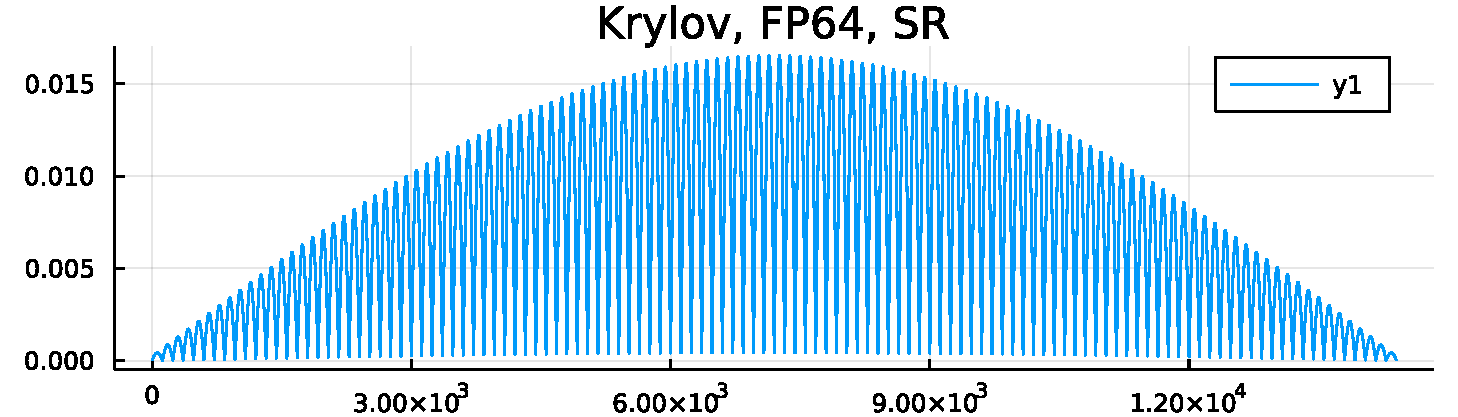
\includegraphics[width=.8\textwidth]{images/vp_fd_laplacien_2D.pdf}
    \caption{Vecteur propre normé de plus petite valeur propre du laplacien à 5 points 2D pour une grille $120\times 120$, le vecteur est donc de dimension 14400. Ici calculé avec une méthode de Krylov en précision double.}
    \label{fig:vp_laplacien_5pt_2D}
\end{figure}


\chapter{Résultats partiels ou connexes}



\section{Optimisation de l'algorithms en fonction du \textit{hardware}}
\label{sec:optim_hardware}
Pour cette section, imaginons que nous disposions d'un algorithme constitué d'un ensemble d'instructions (une instruction consiste typiquement à un ou plusieurs calculs et un stockage dans la mémoire du résultat) numérotées de $1$ à $I$, qui néanmoins doivent être exécutées dans un certain ordre bien précis.


Les données sur lesquelles nous travaillons sont des variables de taille $n$ et d'ordre $k$ avec $k$ pouvant prendre plusieurs valeurs dans un ensemble $\llbracket 0, k_{\text{max}} \rrbracket$. Typiquement, nos variables peuvent être des vecteurs, des matrices, des tenseurs, etc occupant une taille mémoire en rapport avec leur ordre (matrice d'ordre $2$ car stocke $n^2$ nombres, vecteur d'ordre $1$ car $n^1$, etc), et nos opérations des produits matrice-matrice (ordre $k=3$ car nécessite $ \mathcal{O}(n^3)$ produits et sommes de réels), des produits matrice-vecteur (ordre $k=2$ car nécessite $ \mathcal{O}(n^2)$ produits et sommes de réels), des produits scalaire-matrice (ordre $k=2$). Pour exécuter ces instructions nous avons deux agents, chacun ayant des caractéristiques différentes, l'un peut-être plus rapide pour certaines opérations, l'autre plus rapide pour d'autres, ou seulement asymptotiquement, etc.


Lorsqu'un algorithme tel que \ref{alg:conj_grad_pert} a besoin d'être exécuté, supposons avoir le choix pour chaque instruction de demander à l'agent 1 dénoté $A_1$ ou l'agent 2 dénoté $A_2$ d'exécuter l'instruction. On peut répartir les tâches entre les deux agents. Mais il y a un hic: chaque agent dispose de sa propre mémoire sur laquelle il opère exclusivement. La communication est possible entre les deux mémoires mais tout transfert d'information se fait avec un certain coût en temps, qui peut avoisiner voire dépasser l'ordre de grandeur du coût en temps de calcul. 

Nous venons de décrire une situation courante: celle d'un GPU et d'un CPU sur la carte mère. Le GPU est un ensemble d'un grand nombde de processeurs spécialisés qui, s'ils sont correctement utilisés, peuvent se révéler très rapide et efficaces à certains calculs parallélisables, tandis que le CPU est une unité très polyvalente, extrêmement rapide (souvent plus rapidement cadencée que les GPU), mais dont les capacités de parallélisations sont très limitées (souvent quelques c\oe{}urs contre quelques dizaines ou centaines de c\oe{}urs pour un GPU moderne), ce qui peut avoir raison de lui pour les très gros calculs. Si le GPU est très imposant, on pourrait stocker l'entièreté des données de départ et résultats générés sur sa mémoire, c'est le cas le plus favorisé en \textit{machine learning} par exemple, lorsqu'un réseau de neurones complet doit être stocké sur le GPU afin de l'évaluer rapidement, estimer les gradients, et rétropropager le gradient pour l'entraîner. Mais si le GPU est limité, toutes les données en mémoire ne tiennent pas nécessairement.

On impose également que les variables n'aient pas le don d'ubiquité, pour s'interdire tout problème de synchronisation, qui fait partie de l'étude des réseaux.

Le problème devient maintenant clair: paralléliser de gros calculs opérant sur de grosses données est intéressant mais le transfert préalable et ultérieur à un calcul peut changer la donne. Le problème du choix est \textit{a priori} complexe: il existe naïvement $2^I$ paramétrages (deux choix pour chaque instruction).  \textbf{Il est important de noter que ce proglème ne se résout pas facilement par une approche \og diviser pour régner \og. En effet, un optimum global n'est pas constituée d'assemblage d'optima locaux: la raison est que la présence en mémoire d'une variable se propage indéfiniment dans le temps tant qu'elle n'est pas déplacée ou modifiée, expliquant la difficulté principale: les choix antérieurs de déplacement mémoire des variables impactent les étapes ultérieures.}

Je vais décrire une heuristique permettant de trouver une bonne solution  à ce théorème avec quelques autres contraintes évidentes, orientées par le cas des calculs matriciels. Mais l'algorithme est généralisable à des cas moins spécifiques facilement.



On peut donc modéliser la situation par le pseudo-graphe \ref{fig:parcours_GPU_CPU}. Les arêtes représentent les transferts mémoire et les sommets les calculs des instructions (un sommet correspond à une ligne de l'algorithme effectuée sur un processeur. Néanmoins, il ne s'agit pas encore d'un graphe, car le coût en transfert mémoire en passant d'une étape de l'algorithme à une autre dépend du chemin précédemment emprunté, puisque l'on a supposé que les variables ne sont pas omniprésentes et ne sont bougées que lorsque c'est nécessaire. 

\begin{figure}
    \centering
    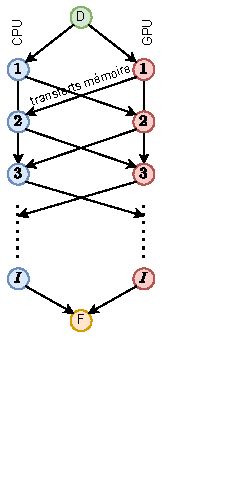
\includegraphics[width=.3\textwidth]{images/CPU_GPU_concept.pdf}
    \caption{Modélisation des  parcours possibles. Dans ce pseudo-graphe, les trajectoires sont mises en avant: ici les arêtes représentent les transferts mémoire et les n\oe{}uds représentent les calculs.}
    \label{fig:parcours_GPU_CPU}
\end{figure}





\subsubsection{Formalisation}
Énumérons les hypothèses
\begin{enumerate}
    \item La taille typique des données est $n$.
    \item Chaque variable est indicée par $v\in \llbracket 1, V \rrbracket$.
    \item Au début, seules les variables utilisées au départ (en entrée de l'algorithme sont allouées dans la mémoire, et sont présentes sur le la mémoire de l'agent $A_1$ (CPU).
    \item Chaque variable est mutable mais typée de type immuable.
    \item Chaque variable $v$ possède en attribut un ordre $k(v) \in \llbracket 0, k_{\text{max}} \rrbracket$.
    \item Chaque instruction est indicée par $i\in \llbracket 1, I \rrbracket$.
    \item Chaque instruction $i$ se compose d'une combinaison linéaire de coûts de  calculs $\kappa_{i,j}$ d'ordres $k(i,j)$ compris dans $\llbracket 1, k_{\text{max}} \rrbracket$.
    \item Chaque calcul $j$ composant une instruction $i$ se fait en un coût $c_{i,j}$ (on s'attend à ce que $c_{i,j} \propto n^{k(i,j)}$) et ainsi $c_i = \sum_j c_{i,j}$.
    \item Il est possible de transférer les variables de la mémoire de l'agent $A_1$ vers celle de l'agent $A_2$ avec un coût proportionnel à l'ordre de la variable.
    \item Une variable n'est transférée avant l'exécution de l'instruction qu'en cas de besoin: pour y accéder lors d'un calcul ou pour faire de la place pour en stocker d'autres sur celle de l'agent $A_2$.
    \item Chaque instruction nécessite certaines variables en accès d'écriture ou de lecture pour effectuer ses calculs.
    \item Toute variable ne peut pas coexister simultanément dans la mémoire de l'agent $A_1$ et de l'agent $A_2$ simultanément.
    \item La mémoire $\mathcal{M}$ de l'agent $A_2$ (GPU) est limitée: $\mathcal{M} < + \infty$.
    \item Chaque variable $v$ occupe une taille mémoire $m_v$ (on s'attend à ce que $m_v \propto n^{k(v)}$).
    \item À chaque étape du calcul on associe son \textit{état final} (état et étape seront donc synonymes), caractérisé uniquement par les variables présentes dans les mémoires respectives des agents $A_1$ et $A_2$ qui restent utiles pour la suite (stricte) de l'algorithme. C'est-à-dire que l'on libère les mémoires des variables dorénavant inutiles à la fin de chaque instruction.
    \item À la fin de l'algorithme, certaines variables sont retournées en sortie de l'algorithme, et doivent être présentes sur la mémoire de l'agent $A_1$ (CPU).
\end{enumerate}

Formalisons tout cela et définissons ainsi:

\begin{itemize}
    \item La matrice $\mathbf{B}\in\mathscr{M}_{(V,I)}(\{0,1\})$ telle que $\mathbf{B}[v,i] = 1$ si et seulement si l'instruction $i$ nécessite l'accès de la variable $v$ en lecture ou écriture.
    
    \item La matrice $\mathbf{K} \in\mathscr{M}_{(k_{\text{max}+1, I})}(\mathbb{N})$ telle que $\mathbf{K}[i,k]$ désigne ne nombre d'opérations d'ordre $k-1$ nécessaires à l'instruction $i$.
    
    \item Le vecteur $\mathbf{D} \in \{0,1\}^V$ tel que $\mathbf{D}[v] = 1$ si et seulement si la variable $v$ fait partie des variables du début (en entrée de l'algorithme).
    
    \item Le vecteur $\mathbf{F} \in \{0,1\}^V$ tel que $\mathbf{F}[v] = 1$ si et seulement si la variable $v$ fait partie des résultats retournés (sorties de l'algorithme).
    
    \item Le vecteur $\mathbf{M}\in \mathbb{R}_+^V$ tel que $\mathbf{M}[v]$ désigne l'occupation mémoire de la variable $v$.
    
    \item Le vecteur $\mathbf{T} \in \mathbb{R}_+^V$ tel que $\mathbf{T}[v]$ désigne le coût d'un transfert de la variable $v$ entre le CPU et le GPU (dans un sens ou dans l'autre).
    
    \item Le vecteur $\mathbf{\Omega} \in \mathbb{N}^V$ tel que $\mathbf{\Omega}[v]$ désigne l'ordre de la variable $v$.
    
    
    \item Le vecteur $\mathbf{\Xi}_{\text{CPU}} \in \mathbb{R}_+^{k_{\text{max}}+1}$ tel que $\mathbf{C}_{\text{CPU}}[k]$ désigne le coût d'une opération d'ordre $k-1$ sur le CPU.
    
    \item Le vecteur $\mathbf{\Xi}_{\text{GPU}} \in \mathbb{R}_+^{k_{\text{max}}+1}$ tel que $\mathbf{C}_{\text{GPU}}[k]$ désigne le coût d'une opération d'ordre $k-1$ sur le GPU.
    
    \item Le vecteur $\mathbf{C}_{\text{CPU}} = \mathbf{K}^\intercal \times \mathbf{\Xi}_{\text{CPU}} \in \mathbb{R}_+^{I}$ tel que $\mathbf{C}_{\text{CPU}}[k]$ désigne le coût de l'étape $i$ de l'algorithme sur le CPU.
    
    \item Le vecteur $\mathbf{C}_{\text{GPU}} = \mathbf{K}^\intercal \times  \mathbf{\Xi}_{\text{GPU}} \in \mathbb{R}_+^{I}$ tel que $\mathbf{C}_{\text{GPU}}[k]$ désigne le coût de l'étape $i$ de l'algorithme sur le GPU.
\end{itemize}

%\subsection{Approche analytique}
% A FAIRE
\subsection{Approche par programmation dynamique}
Une bonne idée pour résoudre le problème serait donc de construire un graphe qui décrive à chaque étape les choix correspondants.  Pour obtenir un graphe, les poids doivent être des constantes. Il faudrait donc \og déplier \fg{} ce pseudo-graphe: on obtiendrait ainsi un arbre binaire pour lequel on aurait relié toutes les feuilles à un dernier n\oe{}ud unique. En pratique, il est  possible que des n\oe{}uds en commun existent, si on aboutir à un même état par deux chemins différents. Il est donc peu judicieux (et peu efficace) de créer le pseudo-graphe en le dépliant. On va alors  le construire directement de manière récursive. \textbf{Remarque importante: dès lors, sur le graphe déplié, les arêtes représenteront les coûts (en transfert mémoire et en calcul tous confondus, par exemple en équivalent de temps pour les deux) tandis que les n\oe{}uds représenteront les états de la mémoire (à profondeur constante) et la progression du calcul (à largeur constante).}

Une fois cela fait, il ne reste plus qu'à trouver le plus court chemin entre le premier n\oe{}ud et le dernier. 

Ce problème fait partie de la \textbf{programmation dynamique}, qui se définit grossièrement par une situation dans laquelle les décisions sont séquentielles et où notre système passe d'un état à un autre au fur et à mesure de ces décisions. Plus particulièrement on a besoin de trouver le plus court chemin dans un \textbf{graphe acyclique}. On peut y parvenir avec l'algorithme de \textsc{Dijkstra}, ou même encore d'une manière asymptotiquement plus efficace, récursivement, comme on le verra.

\subsubsection{Construction du graphe}


%\begin{algorithm}
%\caption{Construction du graphe}
%\label{alg:construction_graphe}
\begin{breakablealgorithm}
  \caption{Construction du graphe des trajectoires de calcul}
  \label{alg:construction_graphe}
\begin{algorithmic}[1]
\Require $I, V, \mathbf{B}, \mathbf{K}, \mathbf{D}, \mathbf{F}, \mathbf{M}, \mathbf{\Omega}, \mathbf{T}, \mathbf{\Xi}_{\text{CPU}},  \mathbf{\Xi}_{\text{GPU}}$
\[\]
\Comment{On note $\mathcal{N} = \times \{0,1\}^{2V}  \times \mathbb{R}^2 \times \mathbb{Z} \times \{"CPU", "GPU"\}$ l'ensemble contenant les n\oe{}uds. Correspond au 6-uplet (présence CPU, présence GPU, occupation mémoire CPU, occupation mémoire GPU, état/profondeur, processeur). On note $p_{\text{CPU}}(i)$ et $p_{\text{GPU}}(i)$ respectivement les vecteurs de présence des variables $1$ à $V$ sur le CPU et le GPU à l'étape $i$.}
\[\]
\Require $h: \mathcal{N} \rightarrow H$ une fonction de hachage injective dans un ensemble $H$ quelconque 
est l'ensemble des arêtes
\Require $\mathcal{D}$ une structure de dictionnaire de type $(\mathcal{K} \rightarrow \mathcal{V})$ où $\mathcal{K} \subset H$ et $\mathcal{V} \subset \mathbb{N}^+$
\Require $\mathcal{Q}$ une structure file (FIFO) de type $\mathcal{N}$
\Require $\mathcal{G}$ une structure de graphe orienté de type $(\mathcal{V} \times \mathcal{E})$ où $\mathcal{V} \subset \mathcal{N}$ est l'ensemble des n\oe{}uds et $\mathcal{E}  \subset \mathbb{N}^+\times \mathbb{N}^+$ 
\Ensure $G = (\mathcal{V} \times \mathcal{E})$ le graphe construit des états possibles de l'algorithme 
\[\]
\[\]
\Procedure{Traitement d'un nouveau n\oe{}ud}{}
\If {$\texttt{haskey}(D, \eta)$} 
        \State $\mathrm{id} \gets D[\eta]$ 
            \State $\texttt{addedgeweight}(G, (\mathrm{id}, s+1), (\mathbf{F} \land \lnot \mathbf{p}_c)^\intercal \mathbf{T})$ 
        \Else 
            \State $\mathrm{id} \gets \mathrm{acc}$ 
            \State $\texttt{addnode}(G, \mathrm{id}, N_\text{new})$ 
            \State $\texttt{addkeyvalue}(D, \eta,  \mathrm{id})$ 
            \State $\texttt{enqueue}(Q, N_{\text{new}})$ 
            \State $\texttt{addedgeweight}(G, (\mathrm{id},2), c)$ 
            \State $\mathrm{acc} \gets \mathrm{acc} + 1$ 
        \EndIf
\EndProcedure
\[\]
\Procedure{Construction en largeur du graphe avec mémoïsation}{}
\State $\mathbf{C}_{\text{CPU}} \gets \mathbf{K}^\intercal \times \mathbf{\Xi}_{\text{CPU}}$
\State $\mathbf{C}_{\text{GPU}} \gets \mathbf{K}^\intercal \times \mathbf{\Xi}_{\text{CPU}}$

\State $G = \mathcal{G}(\emptyset, \emptyset)$ \Comment{Création du graphe}
\State $Q = \mathcal{Q}(\emptyset)$ \Comment{Création de la FIFO des n\oe{}uds}
\State $D = \mathcal{D}(\emptyset)$ \Comment{Création du dictionnaire des n\oe{}uds}
\[\]

\For{$\mathrm{id},\vect{R},s \in \texttt{zip}(\{1, 2\}, \{\mathbf{D}, \mathbf{F}\}, \{0, I+1\})$}
\State $N \gets (\mathbf{R}, \vect{0}^V, \mathbf{M}^\intercal  \mathbf{R}, s, "CPU") \in \mathcal{N}$ \Comment{Création n\oe{}uds départ et arrivée}
\State $\texttt{addnode}(G, \mathrm{id}, N)$ \Comment{Insérer ce n\oe{}ud dans le graphe}
\State $\texttt{addkeyvalue}(D, h(N),\mathrm{id})$ \Comment{Insérer ce n\oe{}ud dans le dictionnaire}
\EndFor
\[\]
\State $\texttt{enqueue}(Q,N)$ \Comment{Enfiler ce n\oe{}ud pour traitement ultérieur}
\State $\mathrm{acc} \gets 3$ \Comment{Accumulateur pour les identifiants (coloration)}
\[\]
\While{$|q| > 0$} \Comment{Tant que la queue est non vide}
\State $N \gets \texttt{dequeue}(q)$ \Comment{Défiler le n\oe{}ud à traiter en place}
\State $(\mathbf{p}_c, \mathbf{p}_g,m_c, m_g, s, t) \gets N$ \Comment{Extraire ses propriétés}
\State $\mathrm{id} \gets D[h(N)]$ \Comment{Déduire son identifiant}

\If {$s = I$} \Comment{S'il s'agit d'une feuille (fin de calcul)}

    \State $\texttt{addedgeweight}(G, (\mathrm{id}, 2), c)$ \Comment{Relier cette feuille au n\oe{}ud final}
\Else
    \State $\vect{b} \gets \mathbf{B}[:,s+1]$ \Comment{Récupérer les variables nécessaires à l'étape suivante}
    \State $\vect{b}_{\text{ult}} = \mathrm{Vect}\{\texttt{Bool}\}((\mathbf{B}[:,s+2:I]|\mathbf{F})  \times \vect{1}^{I-s} .> 0)$ \Comment{$\in \{0,1\}^V$: besoins $\ge s+1$}
    
    \[\]
    
        
    \If $(\vect{b} \lor \vect{p}_g)^\intercal \time \mathbf{M} \le \mathcal{M}$ \Comment{Calcul \& import direct GPU possible}
        \State $\vect{vi} \gets \vect{b} \land \lnot \vect{p}_g$ \Comment{Variables importées sur GPU}
        
        \State $c \gets \vect{vi}^\intercal \mathbf{T} + \mathbf{C}_{\text{GPU}}[s+1]$ \Comment{Coût transferts + calculs GPU}
        

        
        \State $\vect{p}_{g,\text{new}} \gets (\vect{b} \lor  \vect{p}_g) \land \vect{b}_{\text{ult}}$ \Comment{Nouveau vecteur présence GPU}
        
        \State $\vect{p}_{c,\text{new}} \gets (\vect{p}_{c} \land \lnot  \vect{vi}) \land \vect{b}_{\text{ult}}$ \Comment{Nouveau vecteur présence CPU}
        \State $N_{\text{new}} \gets (\vect{p}_{c,\text{new}}, \vect{p}_{g,\text{new}}, \vect{p}_{c,\text{new}}\mathbf{M}, \vect{p}_{g,\text{new}}\mathbf{M}, "GPU")$ \Comment{Créer le n\oe{}ud-fils}
        \State $\eta  \gets h(N_{\text{new}})$ \Comment{Calcul du hash du n\oe{}ud-fils}
        \State $\texttt{traitement}(G, \vect{id}, N_{\text{new}}, D, \eta, c, s, \mathbf{F}, \vect{p}_c, \mathbf{T})$
\[\]
    \ElsIf {$\vect{b}^\intercal \time \mathbf{M} \le \mathcal{M}$} \Comment{Calcul sur GPU possible si mémoire vidée}
        \State $\vect{vie} \gets \vect{b} \oplus  \vect{p}_g$ \Comment{Variables importées ou exportées}
        \State $c \gets \vect{vie}^\intercal \mathbf{T} + \mathbf{C}_{\text{GPU}}[s+1]$ 
        
        \State $\vect{p}_{g,\text{new}} \gets \vect{b} \land \vect{b}_{\text{ult}}$ 
        
        \State $\vect{p}_{c,\text{new}} \gets (\vect{p}_g \lor (\lnot \vect{b} \land \vect{p}_g )) \land \vect{b}_{\text{ult}}$ 
        
        \State $N_{\text{new}} \gets (\vect{p}_{c,\text{new}}, \vect{p}_{g,\text{new}}, \vect{p}_{c,\text{new}}\mathbf{M}, \vect{p}_{g,\text{new}}\mathbf{M}, "GPU")$ 
        \State $\eta  \gets h(N_{\text{new}})$ 
        \State $\texttt{traitement}(G, \vect{id}, N_{\text{new}}, D, \eta, c, s, \mathbf{F}, \vect{p}_c, \mathbf{T})$
    \Else \Comment{Calcul sur CPU seulement possible}
        \State \texttt{nothing}
    \EndIf

\EndIf
\EndWhile
\EndProcedure
\end{algorithmic}
%\end{algorithm}
\end{breakablealgorithm}

\subsubsection{Preuve de terminaison}
L'algorithme \ref{alg:construction_graphe} de création de l'arbre est en tous points similaire à un parcours d'arbre en largeur, avec marquage des sommets explorés (ou ici, créés).
La boucle \texttt{while} est le point délicat qui empêche de trivialiser la preuve de terminaison.

Faisons quelques  remarques:
\begin{enumerate}[label=(\subscript{P}{{\arabic*}})]
    \item Toutes les opérations de l'algorithme (chaque ligne) se font en temps fini donc chaque parcours de la boucle 
    \item Au cours d'un parcours de la boucle, un n\oe{}ud est défilé, sinon l'exécution est terminée.
    \item À cause de la vérification à l'aide de la fonction de hachage, les n\oe{}uds créés sont tous distincts 2 à 2, dans la file, le dictionnaire, ou le graphe.
    
    \item Au cours d'un parcours de la boucle, si un défilement d'un n\oe{}ud d'état $s<I$ a lieu, il y a au moins un et au plus deux enfilement(s) de  n\oe{}uds fils d'état $s+1$ dans la file. 
    \item Dans une boucle, ($\exists$ 1 enfilement et marquage d'un n\oe{}ud d'état $s+1$) $\Longleftrightarrow$ ($\exists$ 1 défilement d'un n\oe{}ud d'ordre $s$).
    \item Tout n\oe{}ud d'état $s\ge I$ ne donne lieu à aucun ajout de nouveau n\oe{}ud dans le graphe et dans le dictionnaire.
\end{enumerate}

\begin{proof}
Par la propriété $P2$, prouver la terminaison de la boucle revient à montrer que la file se videra en temps fini.

Par la propriété $P1$, cela revient à montrer que la file se videra (simplement).

Par les propriétés $P5$ et $P6$, il ne peut pas exister dans la file  des n\oe{}uds d'état $s > I$.

Par la propriété $P4$, on conclut qu'un n\oe{}ud défilé n'est jamais réenfilé, car un n\oe{}ud et un de ses fils diffèrent toujours au moins par leur état.

Par les propriétés $P3$ et $P4$, on peut aussi montrer immédiatement par récurrence qu'il existe au plus $2^s$ n\oe{}uds d'ordre $s$.

Avec ce qui précède et la propriété d'unicité $P3$, on conclut que peuvent exister dans la file et le dictionnaire, au plus $M=\sum_{s=1}^I 2^s$ n\oe{}uds, soit un nombre fini de n\oe{}uds, qui sont tous distincts.

Puisqu'on a montré qu'un n\oe{}ud défilé n'est jamais enfilé à nouveau, qu'ils sont tous disctincts et en nombre fini, et qu'à chaque parcours de la boucle \texttt{while}, un n\oe{}ud est défilé, on conclut que l'ensemble des n\oe{}uds défilés distincts est de cardinal strictement croissant et majoré par $M$ au fur et à mesure des appels de la boucle. Il est donc nécessaire qu'il y ait un nombre fini de parcours de la boucle. On a montré que la file se vide finit par se vider  en temps fini.
\end{proof}




\subsubsection{Preuve de correction?}
Cet algorithme est déjà une heuristique: il n'explore qu'une partie des trajectoires possibles. La raison est que dans le cas où la mémoire GPU est limitée trop occupée pour passer à l'étape suivante, on la vide complètement. Ceci n'est pas forcément toujours nécessaire. Mais modéliser tous les sous-ensemble de variables rapatriées sur la mémoire principale à chaque fois que ce blocage intervient ferait exploser la complexité combinatoire du problème (rajoutant potentiellement $2^{\lnot \mathbf{B}[:,s]}$ fils au n\oe{}ud en train d'être traité au lieu d'un seul avec l'algorithme), sous la contrainte que la mémoire libérée doit suffire à stocker $\mathbf{B}[:,s]$.

Par conséquent l'algorithme ne renvoie pas nécessairement une des trajectoires optimales possibles au sens des coûts.
 
\subsubsection{Majoration optimale  du nombre de n\oe{}uds}



En notant 
\begin{equation}
    k(s) = \# \{v\in\llbracket 1, V \rrbracket, [\mathbf{B}|\mathbf{F}] [v, s+1 : I] \neq \vect{0}^{I-s} \}
\end{equation}
$k(i)$ est le nombre de variables que l'on va réutiliser ultérieurement à la fin de l'instruction/étape $i$.
On a la majoration
\begin{equation}
    \#\{N \in V, \mathrm{prof}(N) = s\} \le 2^{\max (k(s), s)}
\end{equation}

Sans plus de contrainte, cette majoration est optimale avec cette modélisation.
En effet, si l'on choisit $\mathcal{B} = \mathds{I}$ (matrice identité) avec $I=V$ et $\mathbf{F} = (1, 1, 1, \cdots, 1)^\intercal$, et $\mathcal{M} \ge \sum_{v=1}^V \mathbf{M}[v]$. Ce calcul n'a pas beaucoup d'intérêt mais il est facile de voir que l'arbre binaire associé est complet, avec l'ensemble des n\oe{}uds de profondeur $I$  en bijection avec $\{0,1\}^{I}$ de cardinal $2^I$.

\subsubsection{Complexité du parcours}
Pour trouver le plus court chemin entre le premier n\oe{}ud représentant l'état initial $0$, et le dernier représentant l'état final $I+1$, un algorithme naturel et efficace est d'utiliser celui de \textsc{Dijkstra}, dont la complexité pour un graphe orienté pondéré à poids \textbf{positifs} est $\mathcal{O}(E+V\log V)$ soit $\mathcal{O}(I2^I)$ puisque $V\le 2^I$ et $E =\mathcal{O}(V)$.



On peut théoriquement mieux faire: Si l'on déplie le graphe en structure chaînée comme arbre binaire: tout arbre s'écrivant $A = (R, (A_1, c_1), (A_2, c_2))$ (racine, sous-arbre gauche et le poids de l'arête le reliant à la racine $R$, et de même pour le sous-arbre droit). Nous choisissons qu'une feuille est du type $(F, c_f)$ pour une raison que je détaille ci-après.

Alors nous avons $G = (N, (G_c, c_c), (G_g, c_g))$ (N\oe{}ud, sous-arbre gauche ou CPU, sous-arbre droit chacun avec les coûts correspondant à leurs arêtes respectives), dont les feuilles (n\oe{}uds d'arêt) sont du type $(F, c_f)$ affectées d'un coût final (correspond aux arêtes liant les n\oe{}uds de profondeur $I$ et le n\oe{}ud jaune dans la figure \ref{fig:graph_computation}).

On peut alors facilement trouver le chemin le plus court en $\mathcal{O}(2^I)$. En effet, la fonction $T$  \og longueur du chemin le plus court jusqu'au dernier n\oe{}ud du graphe \fg{} poids minimal pour $T(G)$ s'écrit récursivement
\begin{equation}
    T(G) = \min (c_g + T(G_g), c_c + T(G_c))
\end{equation}

Soit, en notant $v$ le nombre de sommets d'un arbre binaire et $C$ la fonction coût d'un appel à $T$:
\begin{equation}
    C(v) = 2C\left( \frac{v}{2} \right) + \mathcal{O}(1)
\end{equation}
Cette relation est bien connue et c'est un cas couvert par le \href{https://en.wikipedia.org/wiki/Master_theorem_(analysis_of_algorithms)}{Master Theorem} et montre que la complexité de $T$ est linéaire avec le nombre de sommets $V$ soit $\mathcal{O}(2^I)$, ce qui constitue une amélioration du parcours de \textsc{Dijikstra}. 

\subsubsection{Un exemple: la fonction $\mathbb{R}^{N^2} \times \mathbb{R}^{N^2} \times \mathbb{R}^N \times \mathbb{R}^N: (R, S, u, v) \mapsto (u^\intercal RS(u+V), Sv)$}
Considérons le cas de l'algorithme suivant avec $n=10$, $k_{\text{max}} = 3$, $\mathcal{M}=2000$.


\begin{algorithm}[H]
\caption{Calcul spécimen sur matrices et vecteurs}
\label{alg:calc_ABuv}
\begin{algorithmic}[1]
\Require $R,S,  u, v$
\Ensure Les résultats des calculs matriciels $v^\intercal RS (u+v)$ et $ Sv$

\State $R \gets RS$ \Comment{$n^3$ produits de scalaires}
\State $u[1] \gets u^\intercal R (u+v)$ \Comment{$n^2 + n$ produits de scalaires}
\State $v \gets Sv$ \Comment{$n^2$ produits de scalaires}


\Return $u, v$
\end{algorithmic}
\end{algorithm}

On définit les matrices et vecteurs précédemment listés qui caractérisent l'algorithme



\begin{equation}
      \mathbf{B}|\mathbf{F} = 
    \begin{blockarray}{ccccc}
        & \mathbf{B}_1 & \mathbf{B}_2 & \mathbf{B}_3 & \mathbf{F}\\[6pt]
      \begin{block}{c(cccc)}
        R: & 1 & 1 & 0 & 0 \\[4pt]
        S: & 1 & 0 & 1 & 0 \\[4pt]
        u: & 0 & 1 & 0 & 1 \\[4pt]
        v: & 0 & 1 & 1 & 1 \\[4pt]
      \end{block}
    \end{blockarray}, \qquad \mathbf{D} = \begin{bmatrix}
1 \\[4pt]
1 \\[4pt]
1 \\[4pt]
1
\end{bmatrix}
\end{equation}
(car au début, les 4 variables d'entrée sont données)

\begin{equation}
      \mathbf{K} = 
    \begin{blockarray}{cccc}
          & 1 & 2 & 3 \\[6pt]
      \begin{block}{c\left(ccc\right)}
\text{ordre 0} & 1 & 1 & 0  \\[4pt]
\text{ordre 1} & 1 & 0 & 1  \\[4pt]
\text{ordre 2} & 0 & 1 & 0  \\[4pt]
\text{ordre 3} & 0 & 1 & 1  \\[4pt]
      \end{block}
    \end{blockarray}
\end{equation}



\begin{equation}
    \mathbf{\Omega} = \begin{bmatrix}
2 \\[4pt]
2 \\[4pt]
1 \\[4pt]
1
\end{bmatrix}, \qquad
\mathbf{M} = \begin{bmatrix}
n^0 \\[4pt]
n^1 \\[4pt]
n^2 \\[4pt]
n^3
\end{bmatrix}, \qquad 
\mathbf{\Xi}_{\text{CPU}} = \begin{bmatrix}
n^0 \\[4pt]
n^1 \\[4pt]
n^2 \\[4pt]
n^3
\end{bmatrix}, \qquad
\mathbf{\Xi}_{\text{GPU}} = \begin{bmatrix}
1.0 \\[4pt]
n^{1-1} \\[4pt]
n^{2-1} \\[4pt]
n^{3-1}
\end{bmatrix}
\end{equation}

(en faisant l'hypothèse que le GPU prarallélise toujours suivant une dimension)

Sur cet exemple, la résolution conduit à créer le graphe \ref{fig:graph_computation}, qui montre que la trajectoire optimale est de l'effectuer sur le GPU en entier, principalement car toutes les variables utiles à tout instant donné occupent une place mémoire inférieure ou égale à la limite du GPU. Avec des exemples plus compliqués, on peut générer des gros graphes ou le GPU devient parfois prohibitif.



\begin{figure}[H]
    \centering
    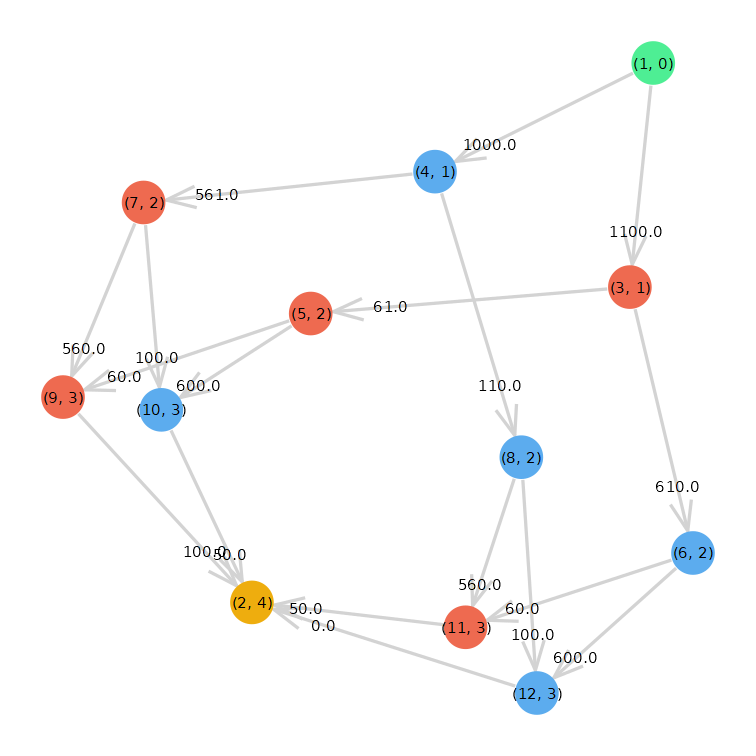
\includegraphics[width=.7\textwidth]{images/graph_computation.png}
    \caption[Graphe des trajectoires de calcul pour l'algorihme \ref{alg:calc_ABuv}]{Graphe acyclique pour l'algorithme \ref{alg:calc_ABuv} avec les paramètres indiqués et  $\mathbb{R}^{N^2} \times \mathbb{R}^{N^2} \times \mathbb{R}^N \times \mathbb{R}^N: (R, S, u, v) \mapsto (u^\intercal RS(u+v), Sv)$ (cas d'école). Chaque n\oe{}ud est ici identifié par un couple $(\texttt{identifiant}, \texttt{profondeur})$ et représente un état du calcul. Sur une ligne de profondeur constante les différents n\oe{}uds représentent les différents scénarios d'états d'occupation de la mémoire. Les arêtes du graphe correspondent aux coûts de calcul et transfert mémoire pour passer d'un état à un autre. L'identifiant correspond à l'ordre d'insertion dans le graphe. Nous avons trois instructions donc bien une profondeur égale à 3. Ici, on voit seulement 4 n\oe{}uds de profondeur 3, chacun d'entre eux étant commun à 2 des $2^3=8$ scénarios  de calcul. Les n\oe{}uds rouges correspondent au GPU et les bleus, au CPU.}
    \label{fig:graph_computation}
\end{figure}





\section{Contrôle de l'erreur de bout en bout}



Je me place dans ce paragraphe dans le cadre où l'on dispose d'un potentiel pour lequel on cherche l'énergie propre et la fonction d'onde de l'état fondamental  non dégénéré, et j'essaie de donner des résultats pour majorer systématiquement tous les types d'erreurs commis (arrondi, troncature, discrétisation). Je me place ici dans l'hypothèse où le pas de discrétisation est le même selon les deux coordonnées généralisées ou deux directions d'espace, et  où seule l'\og ouverture \fg{}\footnote{Pour emprunter le terme à l'optique, par abus.} de la grille, son étendue sur $[x_\text{min},x_\text{max}] \times [y_\text{min},y_\text{max}]$, est adaptable. La raison est que fixer $h$ (pas d'espace) permet de connaître les valeurs propres, et donc le conditionnement, de la matrice du laplacien 2D en différences finies correspondant ce qui simplifie la majoration.

%Et on définit également un vecteur qu'on ne calculera pas mais existe, et qui sert au calcul de l'erreur:
%\begin{itemize}
%    \item $\phi_{(i,j)} \in \mathbb{R}^{N\times N}$ la solution numérique au problème matriciel discrétisé $-\frac{\hbar^2}{2m}\Lambda^\text{2D} \phi = (\hat{\mathcal{E}}-\hat{\mathcal{V}}) \phi$  du laplacien sur la grille en différences finies (problème généralisé aux valeurs propres) avec l'énergie fondamentale \emph{analytiquement exacte} $\mathcal{E}$ (a priori $\phi$ est inaccessible également puisque $\mathcal{E}$ l'est).  
    
%\end{itemize}





\textbf{Dans ce qui suit, je note $\Psi^s_{(i,j)}$ la matrice de $\Psi^s$ échantillonné sur la grille des $(x_i,y_j)$, et $\psi_{(i,j)}$ et $\psi_{(i,j)}$ les matrice définies comme ci-dessus. De même je note $(\Delta\Psi^s)_{(i,j)}$ le laplacien de $\Psi^s$ échantillonné sur la grille. Je note pareillement l'échantillonnage du potentiel (connu) $V \equiv \mathcal{V}(x_i,y_j)$ qui est une matrice diagonale, de même taille que $\Lambda^\text{2D}$, et qui représente sur la grille l'opérateur $\hat{\mathcal{V}}$. Ainsi $\Psi^s$ désigne la fonction et $\Psi^s_{(i,j)}$ désigne la matrice des échantillons sur la grille.} Notons qu'avec ces notations nous avons donc l'égalité vectorielle
\begin{equation}
\label{egalite_vectorielle_hamiltonien_discret_exact}
    -\frac{\hbar^2}{2m}(\Delta\Psi^s)_{(i,j)} + V\Psi^s_{(i,j)} = \mathcal{E}\Psi^s_{(i,j)}
\end{equation}
qui est juste un échantillonnage sur notre grille de la version continue de l'égalité. Je m'en servirai après.


Puis je définis
\begin{itemize}
    \item $\Psi^s \in L^2(\mathbb{R}^2,\mathbb{R})$ la fonction d'onde solution réelle du problème aux valeurs propres continu vérifiant bien-sûr $-\frac{\hbar^2}{2m} \Delta \Psi^s + \hat{\mathcal{V}}\Psi^s = \hat{\mathcal{E}}\Psi^s$ sur tout l'espace avec $\mathcal{E}$ l'énergie propre du fondamental (inaccessible analytiquement a priori);
    
    \item $\psi_{(i,j)} \in \mathbb{R}^{N\times N}$ la solution  au problème matriciel discrétisé $-\frac{\hbar^2}{2m}\Lambda^\text{2D} \psi_{(i,j)} + V \psi_{(i,j)} = E \psi_{(i,j)}$ du laplacien sur la grille en différences finies (problème aux valeurs propres) avec l'énergie fondamentale $E$ (supposément proche de $\mathcal{E}$);
\end{itemize}

Il est à noter qu'en réalité, on calcule numériquement une approximation de $E$ et une approximation de $\psi$, puisqu'on est en grande dimension, on a recours à des méthodes itératives très certainement, cf. les sections précédentes du rapport.



Puis on cherche à estimer naturellement l'erreur
\begin{equation}
     \|\psi_{(i,j)}-\Psi^s_{(i,j)}\|
\end{equation}
avec le sens de cette norme à préciser plus tard (en dimension finie, toutes les normes sont équivalentes donc on pourra passer de l'une à l'autre aisément, je passe de la norme infinie qui représente l'écart maximal, à la norme 2 ensuite).

On va décomposer cette erreur en plusieurs termes pour pouvoir la majorer. Le fait de discrétiser le problème va permettre de trouver une énergie fondamentale approchée $E$ qui comme on l'a dit, est espérer proche de l'énergie du fondamental analytiquement exacte $\mathcal{E}$.  


\subsection{Erreur de discrétisation sur le vecteur}

\paragraph{Première étape: majorer l'erreur faite sur le laplacien}
 En utilisant le théorème \ref{thm_majoration_fct_onde}, on sait que la fonction recherchée est à décroissance rapide au voisinage de $\|(x,y)\| \rightarrow + \infty$, et que $\forall \varepsilon >0, \, \exists c>0, \, \forall x, \, |\psi(x)| \le D \exp(-\frac{1}{2}(c+\varepsilon)^{1/2}|x|^{2})$ pour certains paramètres $D$, $c$, $\varepsilon$. On dénote donc par $\gamma >0$ une fonction dépendant de la taille de la grille (étendue selon $x_\text{max}$ en supposant que $x_\text{max} \sim y_\text{max}$) telle que, en dehors de la grille, $|\psi(x,y)| \le \gamma$. On retient ainsi que $\gamma = \mathcal{O}(e^{-x_\text{max}^2})$. On suppose raisonnablement que $\Psi^s$ est de classe $\mathscr{C}^\infty$ et à décroissance rapide et que ses dérivées sont bornées. Par conséquent, l'approximation du laplacien à 5 points, si elle prenait même les points extérieurs à la grille aux points des frontières en dénotant $(\mathcal{L}\Psi^s)_{(i,j)}$, donnerait une erreur en norme $\infty$ telle que
    
    \begin{equation}
    \label{erreur_laplacien_complet}
        \| (\Delta\Psi^s)_{(i,j)} - (\mathcal{L}\Psi^s)_{(i,j)}\|_\infty \le \frac{h^2}{12} \left( \sup_{\mathbb{R}} \left|\frac{\partial^4 \Psi^s}{\partial x^4}\right| +\sup_{\mathbb{R}} \left|\frac{\partial^4 \Psi^s}{\partial y^4} \right| \right)
    \end{equation}
    
Mais la matrice du laplacien $\Lambda^\text{2D}$ ne prend pas en compte les points extérieurs à la grille. Sur ces points $\Psi^s$ prend des valeurs inférieures ou égales à $\gamma$, donc on va majorer en décomposant en deux termes
\begin{multline}
\label{maj_erreur_laplacien}
    \|\Lambda \Psi^s_{(i,j)} - (\Delta\Psi^s)_{(i,j)} \|_2 \le \underbrace{\|\Lambda \Psi^s_{(i,j)} - (\mathcal{L}\Psi^s)_{(i,j)} \|_2}_{\circled{1}} + \underbrace{\|(\mathcal{L}\Psi^s)_{(i,j)} - (\Delta\Psi^s)_{(i,j)} \|_2}_{\circled{2}}
\end{multline}
Le premier terme est l'erreur d'approximation du laplacien à 5 points, qui tend vers $0$ lorsqu'on raffine le pas de discrétisation; le second terme est l'erreur qu'on commet en ne prenant pas les points en dehors de la grille pour le laplacien des frontières.


On sait que  $\|\cdot \|_2 \le \sqrt{\text{dim}} \| \cdot \|_\infty$, et ici $\text{dim} = N^2$ (puisque nous avons discrétisé sur $N$ points de grille sur chaque axe en 2D).


D'une part, le résultat connu sur la convergence du laplacien à 5 points \ref{erreur_laplacien_complet} permet donc d'écrire en notant
\begin{equation}
    \circled{1} \le N  \cdot \|\Lambda \Psi^s_{(i,j)} - (\mathcal{L}\Psi^s)_{(i,j)} \|_\infty \le   \frac{Nh^2}{12} \left( \sup_{\mathbb{R}} \left|\frac{\partial^4 \Psi^s}{\partial x^4}\right| +\sup_{\mathbb{R}} \left|\frac{\partial^4 \Psi^s}{\partial y^4} \right| \right)
\end{equation}
et je note dorénavant $S =  \sup_{\mathbb{R}} \left|\frac{\partial^4 \Psi^s}{\partial x^4}\right| +\sup_{\mathbb{R}} \left|\frac{\partial^4 \Psi^s}{\partial y^4} \right| $.

D'autre part,  l'erreur que l'on commet en ne prenant pas en compte les valeurs de $\Psi^s$ en dehors de la grille concerne $4N$ points, tous sur lesquels $\Psi^s$ prend des valeurs proches de $0$ à $\gamma$ près, c'est-à-dire qu'on peut en calculer un majorant en norme 2 en sommant le carré de ces erreurs. Chaque erreur individuelle vaut au plus $\frac{\gamma}{h^2}$ en effet, puisque le poids d'un point extracentré dans le laplacien à 5 points est de $\frac{1}{h^2}$:

\begin{equation}
    \circled{2}  \le \sqrt{4N\left(\frac{\gamma}{h^2}\right)^2} = 2\sqrt{N}\frac{\gamma}{h^2}
\end{equation}

On conclut en réinjectant dans \ref{maj_erreur_laplacien}:
\begin{equation}
\label{majorant_erreur_laplacien_solution_exacte}
    \boxed{\|\Lambda \Psi^s_{(i,j)} - (\Delta\Psi^s)_{(i,j)} \|_2 \le \underbrace{ \frac{Nh^2S}{12} + \frac{2\gamma\sqrt{N} }{h^2} }_{\textcolor{blue}{\coloneqq g}}}
\end{equation}

\paragraph{Seconde étape: erreur sur le vecteur de grille}

On écrit ensuite comme des perturbations les éléments numériques $\psi_{(i,j)} = \Psi^s_{(i,j)} + \vect{r}$ et  $E = \mathcal{E} + e$, donc on part de l'égalité solution du problème discret
\begin{equation}
    -\frac{\hbar^2}{2m}\Lambda\psi_{(i,j)} + V \psi_{(i,j)} = E \psi_{(i,j)}
\end{equation}
que l'on réécrit
\begin{equation}
    -\frac{\hbar^2}{2m}\Lambda (\Psi^s_{(i,j)} + \vect{r}) + V(\Psi^s_{(i,j)} + \vect{r}) = (\mathcal{E}+e)(\Psi^s_{(i,j)} + \vect{r}) 
\end{equation}
et réordonne ensuite, avec $E=\mathcal{E}+e$:
\begin{equation}
\label{reordonnement}
    \underbrace{-\frac{\hbar^2}{2m}\Lambda \Psi^s_{(i,j)}  + (V-\mathcal{E})\Psi^s_{(i,j)}}_{\circled{3}} \underbrace{- e \Psi^s_{(i,j)}}_{\circled{4}}  = -\left(-\frac{\hbar^2}{2m}\Lambda +V - E \right)\vect{r} 
\end{equation}
 Cette équation \ref{reordonnement} est une relation que vérifie l'erreur $\vect{r}$ en fonction de l'erreur que l'on fait en approchant le hamiltonien (en fait, la partie du hamiltonien qui corespond au laplacien) et l'énergie. $\vect{r}$ est une quantité vectorielle inaccessible, car $\psi^s$ lui-même est inaccessible: c'est la fonction d'onde qu'on tente d'approcher. La matrice devant $\vect{r}$ dans le terme de droite est singulière par construction, mais son rang est précisément $\vect{dim}-1$ (i.e. $N^2-1$ si l'on est en 2D avec une discrétisation en $N$ points suivant chaque dimension, et $N-1$ si l'on est en 1D). A priori, rien ne permet de dire que $\vect{r} \in \psi_{(i,j)}^\perp$.

Or, comme on a l'égalité \ref{egalite_vectorielle_hamiltonien_discret_exact}, on reconnaît dans \circled{3} une quantité presque nulle d'après l'étape précédente. En effet puisque l'évaluation de $\mathcal{V}$ sur la grille $V$ est exacte (c'est seulement un échantillonnage), et de même pour $\mathcal{E}$ en $E$, l'écart à 0 est seulement dû à l'erreur sur le laplacien en différences finies, majoré dans l'équation  \ref{majorant_erreur_laplacien_solution_exacte}. Ainsi:

\begin{equation}
    \left\| \circled{3} \right\|_2 \le \frac{\hbar^2}{2m} \textcolor{blue}{g}
\end{equation}
et en outre, $\Psi^s_{(i,j)} \le D$ puisque $\Psi^s$ est majoré par $D$:
\begin{equation}
    \left\|\circled{4} \right\|_2 \le eD
\end{equation}

donc le membre de gauche de \ref{reordonnement} est de norme 2 contrôlée par
\begin{equation}
    \left\| -\frac{\hbar^2}{2m}\Lambda \Psi^s_{(i,j)}  + (V-\mathcal{E}I)\Psi^s - e \Psi^s_{(i,j)} \right\|_2 \le \frac{\hbar^2\textcolor{blue}{g}}{2m} + eD
\end{equation}

À partir de là, on ne peut pas facilement déduire une majoration sur $\vect{r}$ car on ne connait pas a priori sa composante sur la direction singulière (droite engendrée par  $\psi_{(i,j)}$) de $-\frac{\hbar^2}{2m}\Lambda +V - E$, qui rend cette matrice singulière.



\subsection{Erreur de troncature sur l'énergie}


Dans \cite{reed_methods_1980}, on peut lire à la fin du chapitre XII, qu'en dimension finie avec les notations précédentes, c'est-à-dire un hamiltonien $H_0$ qu'on perturbe avec $W$ et en notant $(\phi_i)$ (qu'on indice de $1$ à $N$ par convention) les vecteurs propres de $H_0$ associés aux énergies $E_i$, alors l'opérateur

\begin{equation}
    P(\lambda) = -\frac{1}{2 \mathrm{i} \pi} \int_{|E-E_0| = \varepsilon} (H_0 + \lambda W - E )^{-1} \mathrm{d}E
\end{equation}


est la projection sur le vecteur propre de valeur propre $E(\lambda)$ du hamiltonien perturbé $H_0 + \lambda W$. On peut donc tenter d'évaluer numériquement ce projecteur pour obtenir ensuite l'énergie perturbée.

L'ouvrage donne ensuite les formules pour la perturbation $\lambda W$:

\begin{equation}
    E = E_0 + \lambda \frac{\sum_{n=0}^{+\infty} a_n \lambda^n}{\sum_{n=0}^{+\infty} b_n \lambda^n}
\end{equation}
avec en fait $E_0=E_1$ (c'est la plus petite valeur propre, celle de l'état fondamental) et 
\begin{align}
    a_n &= -\frac{(-1)^{n+1}}{2 \mathrm{i}\pi} \int_{|E-E_0| = \varepsilon} \langle \phi_0 | &V(H_0-E)^{-(n+1)} &| \phi_0 \rangle  \, \mathrm{d}E \\
    b_n &= -\frac{(-1)^{n+1}}{2 \mathrm{i}\pi} \int_{|E-E_0| = \varepsilon} \langle \phi_0 | &(H_0-E)^{-1} [V(H_0-E)^{-1}]^n &| \phi_0 \rangle \, \mathrm{d}E
\end{align}

Si on parvient à calculer suffisamment de coefficients, on peut donc obtenir un approximant  de \textsc{Padé} de l'énergie. La difficulté réside dans l'inverse, et dans l'intégrale bien-sûr. Puisque tous les facteurs sauf les inverses sont des constantes, il s'agit de calculer les intégrales

\begin{equation}
    -\frac{(-1)^{n+1}}{2\pi} \int_{0}^{2\pi}  V(H_0-(E_0+\varepsilon e^{\mathrm{i}t})I)^{-(n+1)} \, \mathrm{d}t
\end{equation}
et
\begin{equation}
    -\frac{(-1)^{n+1}}{2 \pi} \int_{0}^{2\pi} (H_0-(E_0+\varepsilon e^{\mathrm{i}t}))^{-1} [V(H_0-(E_0+\varepsilon e^{\mathrm{i}t})I)^{-1}]^n  \, \mathrm{d}t
\end{equation}
 

L'ouvrage donne les calculs des premiers termes et précise que $b_0=1$ et $b_1 = 0$, or comme la seconde intégrale est considérablement moins évidente à calculer, je me concentre dans un premier temps sur la première.

Puisque $H_0$ est symétrique réelle, elle est diagonalisable en base orthonormée. On nomme $P$ sa matrice de passage dans cette base. D'autre part, $(E_0+\varepsilon e^{\mathrm{i}t})I$ est diagonale, c'est une homotétie. Donc $\text{Sp}(H_0-(E_0+\varepsilon e^{\mathrm{i}t})I) = \text{Sp}(H_0) -E_0-\varepsilon e^{\mathrm{i}t} = \{E_1 - E_0-\varepsilon e^{\mathrm{i}t}, E_2 -E_0-\varepsilon e^{\mathrm{i}t}, \cdots, E_N-E_0-\varepsilon e^{\mathrm{i}t}\}$. Notons $D = \text{diag}(E_1, \cdots, E_N)$.
Alors toujours en notant $E=E_0+\varepsilon e^{\mathrm{i}t}$, on a pour tout $n$ entier naturel: on a
\begin{equation}
    (H_0-E)^{-n} = (PDP^{-1}-E)^{-1} = P(D-E)^{-n}P^{-1}
\end{equation}


$D-E$ est facile à inverser:
\begin{equation}
    (D-E)^{-1} = \text{diag}\left( \frac{1}{E_i-E_0-\varepsilon e^{\mathrm{i}t}}\right) ; \qquad (D-E)^{-n} = \text{diag}\left( \frac{1}{(E_i-E_0-\varepsilon e^{\mathrm{i}t})^n}\right)
\end{equation}
 et on peut aussi facilement calculer l'intégrale sur $t$ de $(D-E)^{-n}$ avec la formule de \textsc{Cauchy}:
 
 
 \begin{equation}
     \int_0^{2\pi} \frac{1}{(E_i-E_0-\varepsilon e^{\mathrm{i}t})^n} \mathrm{d}t = \int_0^{2\pi} \frac{1}{(E_i-E_0-\varepsilon e^{\mathrm{i}t})^n} \mathrm{d}t
 \end{equation}
\end{appendices}

\nocite{*}
\bibliographystyle{alpha} %abbrv % alpha % unsrt
\bibliography{biblio.bib} 

\end{document}   


